
\documentclass[master]{thesis-uestc}

\title{数字相控阵单脉冲测向方法研究}{The Research on Monopulse estimation with 
Digital Phased Array}

\author{邓宇昊}{Yuhao Deng}
\advisor{谢菊兰\chinesespace 副教授}{Dr. Julan Xie}
\school{信息与通信工程学院}{School of Information and Communication Engineering}
\major{信号与信息处理}{Signal and Information Processing}
\studentnumber{201821011229}

\begin{document}

\makecover

\begin{chineseabstract}
单脉冲测向技术经过近几十年的发展,已经取得了长足的进步。相比于其他测向方法,单脉冲测向方法有着计算复杂度较低、
结构简单和便于工程实现等优点。因此,本文将对相控阵系统中的单脉冲测向方法展开深入细致的研究,主要内容具体如下:

本文首先针对数字相控阵进行建模,包含常见的规则相控阵,即均匀线阵、均匀面阵和均匀圆阵,以及非规则阵列,即共形阵。
我们给出了不同阵列的信号模型,并介绍与之相关的波束形成技术,以及三种传统单脉冲测向方法,
包括半阵法、加权法和比幅测向方法。本文分析传统单脉冲测向方法的优缺点及其使用范围。

接下来,本文针对相控阵系统中的强旁瓣干扰场景展开研究,介绍了三种抑制旁瓣干扰的方法,分别从静态和差波束权优化的角度,
和广义旁瓣对消的角度来解决强旁瓣干扰。针对第一类静态和差波束权优化方法,我们研究了线性规划方法和差分进化算法,
分别从凸优化的角度和遗传算法的角度阐述了低旁瓣和差波束权设计的问题,与加权法类似,这类方法也是事先设计出和差波束权权向量,
拟合出单脉冲比曲线,再将去用于测向。而广义旁瓣对消则不同,它需要依赖一个已有的静态权(比如半阵法的和差波束权),
借助辅助阵列,使得期望信号被辅助阵列阻塞,而旁瓣干扰则可以无失真的通过,进一步在输出端叠加主阵列输出和辅助阵列输出,
使得旁瓣干扰叠加相消。在广义旁瓣对消中,阻塞矩阵的选择也是一个重要的影响因素,因此我们还研究了一种基于SVD和准矩阵的
阻塞矩阵设计方法,并将其用于旁瓣对消器,抑制和差波束中的旁瓣干扰。

然后,我们进一步研究了自适应单脉冲测向方法,并探究了主瓣干扰的影响。与静态权方法不同,自适应带脉冲测向方法是一种在线实时算法,
充分利用了干扰叠加噪声的统计特性。以最大似然方法为代表,利用干扰叠加噪声的概率密度函数,构建对数似然函数,再用牛顿法求解。
MVAM自适应测向方法则是预设理想的单脉冲比,然后对接收信号的单脉冲比做近似处理,并将其在波束指向处做一阶泰勒展开,
经过一系列处理后还原出理想单脉冲比,并将其用于测向。同样的,MVAM方法也需要一个静态和差波束权权,参与自适应测向过程。
此外,为专门应对主瓣干扰,本文还研究了一种正交置零方法,该方法利用了均匀面阵中方位角通道和俯仰角通道相移因子的可分离特性,
使两正交通道相互在主瓣干扰处置零,从而抑制主瓣干扰。除此之外,本文还研究了一种基于LCMV结构和MVDR波束形成的多点约束方法,
该方法约束单脉冲比,使其与期望信号入射角度满足线性关系,在抑制主旁瓣干扰的同时,估计出期望信号的入射角度。
由于其约束点较少,因此当测角范围较宽时,远离约束点处的测角精度就会下降,同时受限于阵列自由度,无法随意增加约束点。
因此,本文针对该方法进行改进,利用SVD近似原约束矩阵,在提高测角精度的同时,尽可能的减少阵列自由度的消耗。

最后,本文将单脉冲测向拓展到极化域,研究了极化相控阵的单脉冲测向方法。首先探究了极化相控阵的信号模型,
利用极子的部署方式,我们将其分为两类,即正交极子的极化相控阵和任意极子的极化相控阵。针对第一类正交极子相控阵,
我们研究了一种双通道信息融合的单脉冲测向方法,该方法利用正交极子各通道间的独立性,分别得出各通道的测向结果后,
做加权融合,得到最终的估计结果。而针对第二类任意极子极化相控阵,本文提出了一种空域-极化域联合估计方法,
该方法从干扰叠加噪声的统计特性入手,构造似然函数,并将极化分量与空域导向向量分离,借助对数似然函数和牛顿公式,
先估计出信号的入射角度,再估计其极化参数。

\chinesekeyword{相控阵,单脉冲,测向,极化敏感阵列}
\end{chineseabstract}

\begin{englishabstract}
This is abstract.

\englishkeyword{key, words}
\end{englishabstract}

\thesistableofcontents

\thesischapterexordium

\section{研究工作的背景与意义}

\section{单脉冲方法的国内外研究历史与现状}
时域积分方程方法的研究始于上世纪60 年代,

\section{本文的主要贡献与创新}
本论文以时域积分方程时间步进算法的数值实现技术、后时稳定性问题以及两层平面波加速算法为重点研究内容,主要创新点与贡献如下:

\section{本论文的结构安排}
本文的章节结构安排如下:

\chapter{相控阵单脉冲测向基本理论}
本章将介绍相控阵单脉冲测向的基本原理,首先在第一节中给出几种相控阵的接收信号模型,然后在第二节中介绍波束形成技术,
最后在第三节中分析三种常用的传统单脉冲测向方法。在本章中,所有入射信号都假设为远场窄带信号,
构成阵列的所有天线均为完全一致且理想的全向天线,没有幅相误差,不考虑阵元间互耦。

\section{相控阵接收信号模型}
依据相控阵阵元天线的排布方式,我们可以将相控阵划分为规则阵和共形阵。
前者主要有均匀线阵、均匀面阵和均匀圆阵,而后者代指天线排布没有特定几何规律的“一般”阵列。
对于远场窄带信号,其一般表达式为$s(t)=A(t)\exp\left[-j\left(2\pi ft+\varphi(t)\right)\right]$,
其中$A(t)$为入射信号的振幅,$\varphi(t)$为初相位。
对于入射信号波程差引起的短时延$\tau$,远场窄带信号有式\eqref{approx}成立。
\begin{equation}\label{approx}
\begin{aligned}
    A(t-\tau) &\approx A(t) \\
    \varphi(t-\tau) &\approx \varphi(t)
\end{aligned}
\end{equation}
因此我们可以忽略时延$\tau$对信号振幅和初相位的影响。
若假设阵列由$M$个阵元组成,则可以得到第$m$个阵元相对于阵列参考点的输出
$s(t)\exp\left(-j2\pi f\tau_m\right)$。
我们进一步将$M$个阵元的输出信号重写为向量形式$\bm{y}$,并且假设每个阵元的噪声都是独立同分布的
零均值高斯白噪声,即$\bm{n}\sim\mathcal{N}\left(0,\sigma^2_n\bm{I}\right)$。
利用上述假设,相控阵接收信号模型可以被表述为式\eqref{data_model}。
\begin{equation}\label{data_model}
    \begin{aligned}
        \bm{y} = s(t)\bm{a} + \bm{n}
    \end{aligned}
\end{equation}
式\eqref{data_model}中,向量$\bm{a}\in\mathbb{C}^{M\times1}$称为导向向量,
是一个与信号入射方向以及阵元排布方式有关的向量。
在接下来的小节中,我们将讨论不同阵列的导向向量。

\subsection{均匀线阵}
均匀线阵是指阵列的所有阵元等间距分布在一条线(如$x$轴)上的阵列。
在本节中我们设相邻两阵元的间距为$d$。
若考虑一远场窄带信号$s(t)$,以俯仰角$\phi$入射到由$M$个阵元组成的均匀线阵上,
如图\ref{ULA}所示。
\begin{figure}[h]
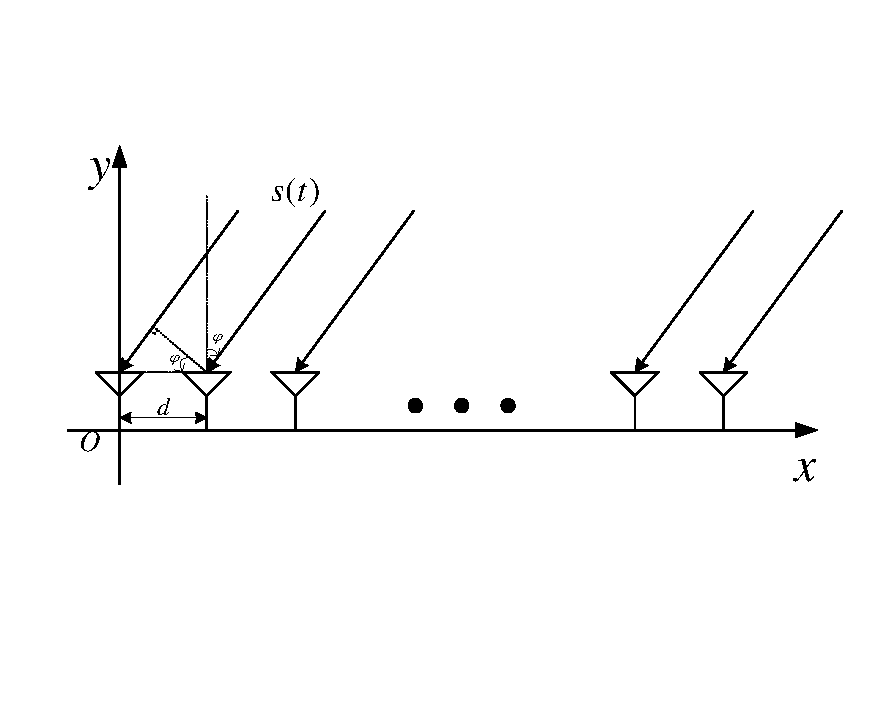
\includegraphics[scale=0.8]{pic/ULA.pdf}
\caption{均匀线阵接收信号模型}
\label{ULA}
\end{figure}

对于均匀线阵,俯仰角$\phi$的定义域通常为$\phi\in\left(-90^\circ,90^\circ\right)$。
设阵列参考点为$O$,即左起第一个阵元。由几何关系我们可以得知,第$m$个阵元相对于参考点的波程差为
$(m-1)d\sin\phi$,因此我们可以得到第$m$个阵元相对于参考点的时延$\tau_m$。
\begin{equation}\label{time_delay}
    \begin{aligned}
    \tau_m = \frac{(m-1)d\sin\phi}{c}
    \end{aligned}
\end{equation}
利用式\eqref{time_delay},均匀线阵的导向向量可以由式\eqref{sv_ULA}表出。
\begin{equation}\label{sv_ULA}
    \begin{aligned}
        \bm{a}(\phi) = 
        \left[
        1,
        \exp\left(j\frac{2\pi d\sin\phi}{\lambda}\right),
        \cdots,
        \exp\left(j\frac{2\pi(M-1)d\sin\phi}{\lambda}\right)
        \right]^T
    \end{aligned}
\end{equation}

在均匀线阵中,要求相邻两阵元间距$d\leq\lambda/2$,否则会造成相位混叠,进而影响单脉冲测向。

\subsection{均匀面阵}
均匀面阵是指所有阵元分布在一个矩形平面如$xOy$平面上,所有阵元共面。
其$x$轴方向上的任意两相邻阵元间距均为$d_x$,
$y$轴方向上的任意两相邻阵元间距均为$d_y$,如图\ref{URA}所示。
\begin{figure}[h]
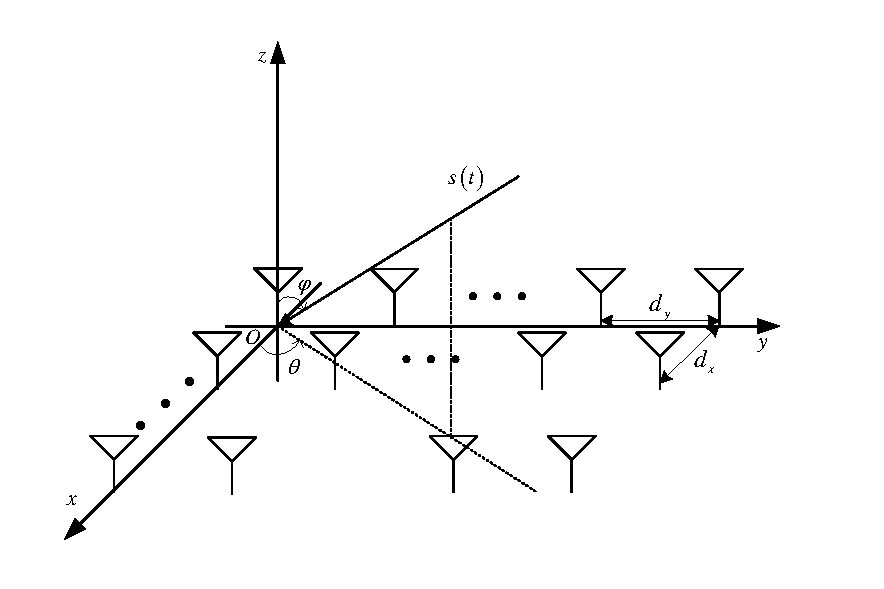
\includegraphics[scale=0.8]{pic/URA.pdf}
\caption{均匀面阵接收信号模型}
\label{URA}
\end{figure}

图\ref{URA}中,期望信号$s(t)$以方位角$\theta$和俯仰角$\phi$入射到该均匀面阵上。
一般情况下,方位角$\theta$的定义域取$\theta\in\left[-180^\circ,180^\circ\right)$,
俯仰角的定义域取$\phi\in\left[0^\circ,90^\circ\right)$。
若假设该均匀面阵共有$M \times N$个阵元,其中$x$轴方向上$M$行,$y$轴方向上$N$列。
依照几何关系依旧可以得到第$(m,n)$个阵元相对于参考点的波程差,进一步得到时延$\tau_{m,n}$。
\begin{equation}\label{URA_time_delay}
    \begin{aligned}
        \tau_{m,n} = 
        \frac{(m-1)d_x\sin\phi\cos\theta + (n-1)d_y\sin\phi\sin\theta}{c}
    \end{aligned}
\end{equation}

因此可以构造一个$M \times N$的矩阵$\bm{S}$,它的第$m$行,
第$n$列元素是第$(m,n)$个阵元相对于参考点的相位差,
即\eqref{URA_phase_delay}式。
\begin{equation}\label{URA_phase_delay}
    \begin{aligned}
        \left[\bm{S}\right]_{m,n} = 
        \exp\left(j\frac{2\pi}{\lambda}
                  \left[(m-1)d_x\sin\phi\cos\theta + (n-1)d_y\sin\phi\sin\theta\right]\right)
    \end{aligned}
\end{equation}
我们利用上一节中均匀线阵的导向向量形式\eqref{sv_ULA},
可以将矩阵$\bm{S}$重写为\eqref{sv_mat_URA}式。
\begin{equation}\label{sv_mat_URA}
    \begin{aligned}
        \bm{S}(\theta,\phi) = \bm{a}_x\bm{a}^T_y
    \end{aligned}
\end{equation}
式\eqref{sv_mat_URA}中,向量$\bm{a}_x\in\mathbb{C}^{M\times1}$和$\bm{a}_y\in\mathbb{C}^{N\times1}$
分别为$x$轴方向和$y$轴方向上均匀线阵形式的导向向量,
其定义由式\eqref{subsv_URA}表出。
\begin{subequations}\label{subsv_URA}
    \begin{align}
        \left[\bm{a}_x\right]_{m} &= 
        \exp\left(j\frac{2\pi(m-1)d_x\sin\phi\cos\theta}{\lambda}\right)
        \\
        \left[\bm{a}_y\right]_{n} &= 
        \exp\left(j\frac{2\pi(n-1)d_y\sin\phi\sin\theta}{\lambda}\right)
    \end{align}
\end{subequations}

最后,我们将矩阵$\bm{S}$按列优先重排得到均匀面阵的导向向量$\bm{a}\in\mathbb{C}^{MN\times1}$。
\begin{equation}\label{sv_URA}
    \begin{aligned}
        \bm{a}(\theta,\phi) = \text{vec}\left(\bm{a}_x\bm{a}_y^T\right)
    \end{aligned}
\end{equation}
上式中,$\text{vec}(\cdot)$表示按列优先重排向量。

\subsection{均匀圆阵}
均匀圆阵指阵列中的所有阵元都均匀分布在一个半径为$R$的圆上,且所有阵元共面。
通常情况下,以圆心$O$作为阵列参考点,如图\ref{UCA}所示。
\begin{figure}[h]
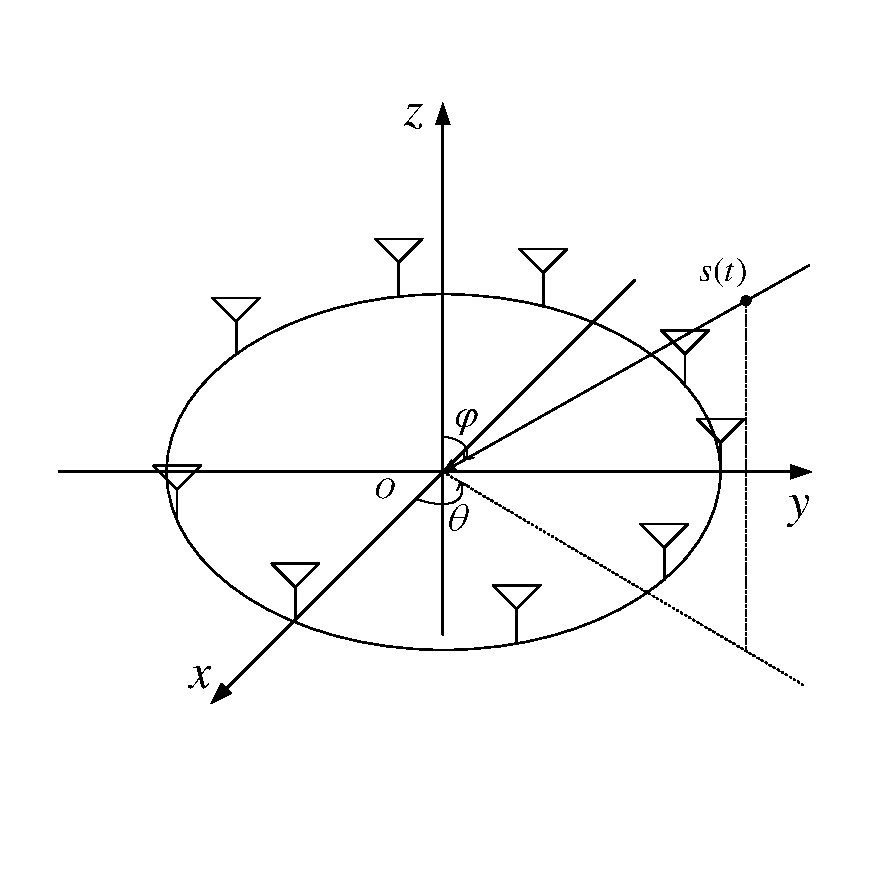
\includegraphics[scale=0.8]{pic/UCA.pdf}
\caption{均匀圆阵接收信号模型}
\label{UCA}
\end{figure}

假设一期望信号以方位角$\theta$,俯仰角$\phi$入射到$M$个阵元组成的均匀圆阵上。
由于$M$个阵元均分圆周,即任意两相邻两阵元的圆弧长相等,
因此我们可以得到第$m$个阵元的坐标$\bm{r}_m$。
\begin{equation}\label{pos_UCA}
    \begin{aligned}
        \bm{r}_m = \left[
            R\cos\varphi_m,
            R\sin\varphi_m,
            0
           \right]^T 
    \end{aligned}
\end{equation}
式\eqref{pos_UCA}中,$\varphi_m$表示第$m$个阵元与$x$轴的夹角,
我们限定其定义域为$\varphi_m\in\left[-\pi,\pi\right)$,
然后给出$\varphi_m$的表达式\eqref{angle_UCA}。
\begin{equation}\label{angle_UCA}
    \begin{aligned}
        \varphi_m = 2\pi\frac{-(M-1)/2+m-1}{M}
    \end{aligned}
\end{equation}

利用$\bm{r}_m$和入射信号角度可以计算出第$m$个阵元相对于参考点$O$的波程差,
进一步得到均匀圆阵导向向量$\bm{a}\in\mathbb{C}^{M\times1}$。
该导向向量的元素由式\eqref{sv_UCA}表出。
\begin{equation}\label{sv_UCA}
    \begin{aligned}
        \left[\bm{a}(\theta,\phi)\right]_m 
        &= 
        \exp\left[j\frac{2 \pi R}{\lambda}
                  \left(
                  \cos\varphi_m\sin\phi\cos\theta + 
                  \sin\varphi_m\sin\phi\sin\theta
                  \right)
            \right]
            \\
        &=    
            \exp\left[
            j\frac{2\pi R}{\lambda}\sin\phi
            \cos\left(\theta-\varphi_m\right)
            \right]
    \end{aligned}
\end{equation}

\subsection{共形阵}
共形阵没有特定的几何规则,导向向量往往与参考点的选取有关。
考虑一个远场窄带信号$s(t)$,以方位角$\theta$和俯仰角$\phi$入射到由$M$个阵元组成的共形阵上,
如图\ref{conformal_array}所示。
\begin{figure}[h]
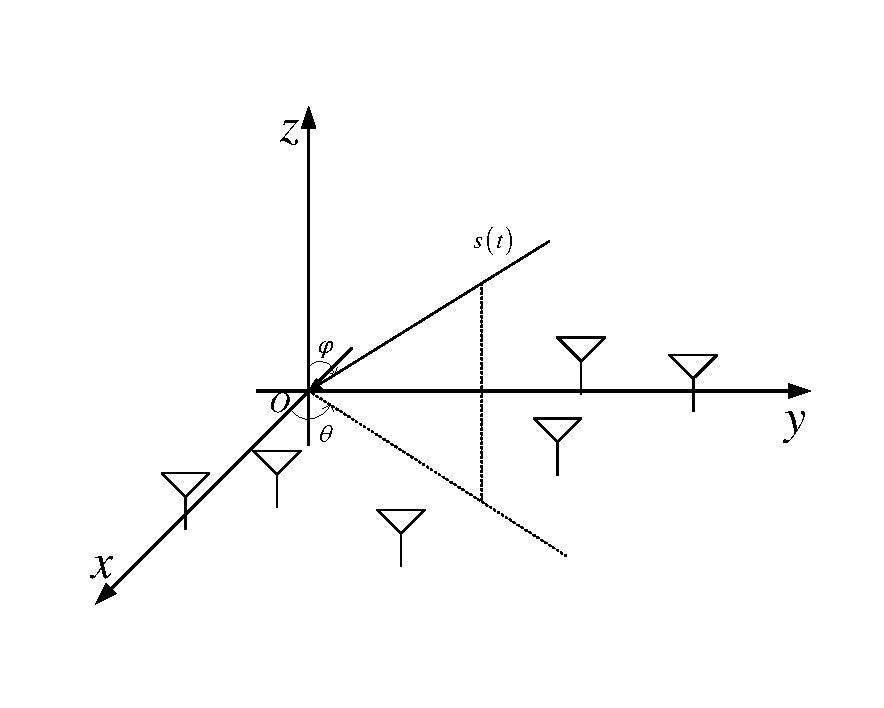
\includegraphics[scale=0.8]{pic/conformal_array.pdf}
\caption{共形阵接收信号模型}
\label{conformal_array}
\end{figure}
假设共形阵的参考点为坐标原点$O$,第$m$个阵元的位置向量为$\bm{r}_m=\left[x_m,y_m,z_m\right]^T$。
入射信号的方向向量由式\eqref{dir_vec}给出。
\begin{equation}\label{dir_vec}
    \bm{\epsilon}_p=-\left[\sin\phi\cos\theta,
                                   \sin\phi\sin\theta,
                                   \cos\phi\right]^T
\end{equation}
因此,我们可以得到第$m$个阵元相对于参考点$O$的相位差$u_m$
\begin{equation}\label{delay}
    \begin{aligned}
        u_m = \exp\left(-j\frac{2\pi}{\lambda}\bm{r}_m^T\bm{\epsilon}_p\right)
    \end{aligned}
\end{equation}
进一步得到共形阵的导向向量$\bm{a}\in\mathbb{C}^{M\times1}$。
\begin{equation}\label{sv}
    \begin{aligned}
        \bm{a}\left(\theta,\phi\right) = 
        \left[\exp\left(-j\frac{2\pi}{\lambda}\bm{r}_1^T\bm{\epsilon}_p\right),
              \exp\left(-j\frac{2\pi}{\lambda}\bm{r}_2^T\bm{\epsilon}_p\right),
              \cdots,
              \exp\left(-j\frac{2\pi}{\lambda}\bm{r}_M^T\bm{\epsilon}_p\right)\right]^T
    \end{aligned}
\end{equation}

式\eqref{sv}是相控阵导向向量的一般表达式,前几个小节中的规则阵列导向向量均可以使用式\eqref{sv}表出。

\section{波束形成技术}
波束形成技术是一种相控阵的空域处理技术,其主要目的是让阵列形成指向,
使得阵列接收信号功率集中于目标方向附近,同时抑制非目标方向的干扰。
波束形成的主要原理是通过对阵列中的各个阵元的输出信号进行加权补相并求和,
使得目标方向上的相位叠加增强,而非目标方向上的相位叠加相消。
让阵列对准目标方向,形成一个指向目标的“波束”,同时对于其余方向上的干扰以及噪声有一定抑制。
在本章中,我们将以半波长间距的均匀线阵为例,分析波束形成的原理和一般过程。

\subsection{MVDR波束形成方法}
MVDR方法即最小方差无失真响应方法,本节我们将以单信源入射均匀线阵为例分析其原理。
考虑一期望信号$s(t)$由方向$\phi_0$入射到$M$阵元的均匀线阵上,
由式\eqref{data_model}知$M$个阵元的输出记为向量$\bm{y}$。
现假设有一$M$个抽头的空域滤波器,其权向量为$\bm{w}\in\mathbb{C}^{M\times1}$。
阵列的输出信号通过该滤波器的输出为$z$,由式\eqref{filter_model}表出。
\begin{equation}\label{filter_model}
    \begin{aligned}
    z = \bm{w}^H\bm{y} = \bm{y}^T\bm{w}^*
    \end{aligned}
\end{equation}
上式中,$\cdot^*$表示转置。
利用式\eqref{filter_model}可以得到该滤波器输出的平均功率$\sigma^2$。
\begin{equation}\label{mvdr_var}
    \begin{aligned}
    \sigma^2 &= E\left\{|z|^2\right\} \\
             &= E\left\{\bm{w}^H\bm{y}\bm{y}^H\bm{w}\right\} \\
             &= \bm{w}^H\bm{Q}\bm{w}
    \end{aligned}
\end{equation}
式\eqref{mvdr_var}中,矩阵$\bm{Q}=E\left\{\bm{y}\bm{y}^H\right\}$
是干扰叠加噪声(即不含有期望信号)的协方差矩阵。

由于期望信号的入射方向是$\phi_0$,利用式\eqref{data_model}和式\eqref{filter_model}可知,
理想情况下(不考虑噪声)滤波器的输出应该是式\eqref{filter_obj}中的$z_0$。
\begin{equation}\label{filter_obj}
    \begin{aligned}
    z_0 = \bm{w}^H\bm{y}(\phi_0) = \bm{w}^H\bm{a}(\phi_0)s(t)
    \end{aligned}
\end{equation}
由于我们要求空域滤波器在目标方向上无失真的通过,因此我们可以令约束条件为式\eqref{constraint}。
\begin{equation}\label{constraint}
    \begin{aligned}
    \bm{w}^H\bm{a}(\phi_0) = 1
    \end{aligned}
\end{equation}
同时,为了抑制其他方向上的干扰和噪声,我们还需要使得滤波器输出的平均功率最小,
因此,该波束形成问题可以表述为一个带约束条件的优化问题,如式\eqref{MVDR_obj}所示。
\begin{equation}\label{MVDR_obj}
    \begin{aligned}
    &\min_\bm{w} ~ \bm{w}^H\bm{Q}\bm{w} \\
    &\text{s.t.} ~ \bm{w}^H\bm{a}(\phi_0) = 1
    \end{aligned}
\end{equation}

我们可以用拉格朗日乘子法求解该问题,首先构造代价函数$J(\bm{w})$。
\begin{equation}
    \begin{aligned}
    J(\bm{w}) = \bm{w}^H\bm{Q}\bm{w} + \mu\left(\bm{w}^H\bm{a}(\phi_0)-1\right)
    \end{aligned}
\end{equation}
然后对代价函数$J(\bm{w})$求梯度,并令其等于$\textbf{0}$向量。
\begin{equation}\label{cost_grad}
    \begin{aligned}
    \nabla J(\bm{w}) = 2\bm{Q}\bm{w} - 2\bm{a}(\phi_0) = \textbf{0}
    \end{aligned}
\end{equation}
求解式\eqref{cost_grad}我们可以得到$\bm{w}$的解。
\begin{equation}\label{w_mu}
    \begin{aligned}
    \bm{w} = \mu\bm{Q}^{-1}\bm{a}(\phi_0)
    \end{aligned}
\end{equation}
注意式\eqref{w_mu}中,只要干扰信号是非相干的,那么协方差矩阵$\bm{Q}$一定可逆。
本小节中只存在一个期望信号,无干扰,而我们假设每个阵元的噪声都是独立同分布的高斯白噪声,
此时矩阵$\bm{Q}$一定可逆。
然后将式\eqref{w_mu}代入式\eqref{constraint},我们可以得到拉格朗日乘子$\mu$。
\begin{equation}\label{larg_arg}
    \begin{aligned}
    \mu = \frac{1}{\bm{a}^H(\phi_0)\bm{Q}^{-1}\bm{a}(\phi_0)}
    \end{aligned}
\end{equation}
最后,我们将式\eqref{larg_arg}代入\eqref{w_mu},得到MVDR权向量的最优解$\bm{w}_o$。
\begin{equation}\label{w_solve}
    \begin{aligned}
    \bm{w}_o = \frac{\bm{Q}^{-1}\bm{a}(\phi_0)}{\bm{a}^H(\phi_0)\bm{Q}^{-1}\bm{a}(\phi_0)}
    \end{aligned}
\end{equation}

MVDR方法要求干扰源的个数小于或等于$M-1$,否则将会导致协方差矩阵$Q$的退化,
我们将$M-1$称为阵列的自由度。对于满足各态历经性的信号$\bm{y}$,我们可以用时间平均估计出其统计平均,
并由此得到协方差矩阵的估计量。

\subsection{LCMV波束形成方法}
MVDR方法的局限性在于,它只有一组约束条件,即期望信号无失真通过。
当阵列需要在多个方向上形成波束,或者在指定方向上形成零点抑制干扰时,MVDR方法就无法胜任这一工作了。
因此在本小节中,我们将介绍一种线性约束最小方差方法,即LCMV方法。

LCMV方法的基本原理相同,我们仍旧需要使空域滤波器的平均输出功率最小,但此时约束条件发生了改变。
假设一个$M$阵元的均匀线阵,
若需要形成$L$个波束,在$\phi_1,\phi_2,\cdots,\phi_L$方向上保持接收信号的单位增益,
同时需要形成$P$个零陷,在$\phi_{L+1},\phi_{L+2},\cdots,\phi_{L+P}$方向上形成零陷用于抑制干扰。
此时,我们可以将多个约束条件写成矩阵乘法的形式,如式\eqref{LCMV_constraint}所示。
\begin{equation}\label{LCMV_constraint}
    \begin{aligned}
        \bm{C}^H\bm{w} = \bm{f}
    \end{aligned}
\end{equation}
上式中,矩阵$\bm{C}\mathbb{C}^{M\times(L+P)}$称为约束矩阵,向量$\bm{f}\in\mathbb{C}^{(L+P)\times1}$
为对应的约束向量。对于上述约束条件,我们可以将其表述为式\eqref{costraint_mat_vec}。
\begin{subequations}\label{costraint_mat_vec}
    \begin{align}
        \bm{C} &= \left[\bm{a}(\phi_1), \cdots, \bm{a}(\phi_L), 
                        \bm{a}(\phi_{L+1}), \cdots, \bm{a}(\phi_{L+P})\right]
        \\
        \bm{f} &= \left[1, \cdots, 1, 0, \cdots, 0\right]^T
    \end{align}
\end{subequations}
类似于MVDR方法,我们依旧可以将该问题表述为一个带约束条件的优化问题,即式\eqref{LCMV_obj}。
\begin{equation}\label{LCMV_obj}
    \begin{aligned}
        &\min_\bm{w} ~ \bm{w}^H\bm{Q}\bm{w} \\
        &\text{s.t.} ~ \bm{C}^H\bm{w} = \bm{f}
    \end{aligned}
\end{equation}
同样利用拉格朗日乘子法构造代价函数,并令其梯度为$\textbf{0}$向量,然后解得
\begin{equation}\label{LCMV_w_mu}
    \begin{aligned}
    \bm{w} = \frac{1}{2}\bm{Q}^{-1}\bm{C}\bm{\mu}
    \end{aligned}
\end{equation}
注意,上式中的向量$\bm{\mu}$是拉格朗日乘子,然后将式\eqref{LCMV_w_mu}代入式\eqref{LCMV_constraint}中
得到
\begin{equation}\label{LCMV_mu}
    \begin{aligned}
        \bm{\mu} = 2\left(\bm{C}^H\bm{Q}^{-1}\bm{C}\right)^{-1}\bm{f}
    \end{aligned}
\end{equation}
最后将式\eqref{LCMV_mu}代入式\eqref{LCMV_w_mu}得到LCMV的最优权向量$\bm{w}_o$,由式\eqref{LCMV_w_opt}表出。
\begin{equation}\label{LCMV_w_opt}
    \begin{aligned}
        \bm{w}_o = \bm{Q}^{-1}\bm{C}\left(\bm{C}^H\bm{Q}^{-1}\bm{C}\right)^{-1}\bm{f}
    \end{aligned}
\end{equation}

与MVDR方法一样,LCMV也存在阵列自由度$M-1$,约束条件的个数$L+P \leq M-1$,
否则将会引起协方差矩阵$Q$的退化。实际上,MVDR方法是LCMV方法的一种特殊情况,
即约束条件的个数只有一个。LCMV方法给出了一种广义形式,在后续的自适应单脉冲测向中,
我们还会用到该方法。

\section{传统单脉冲方法}
在上一节中,我们假设波束形成的方向$\phi_0$和期望信号的真实方向$\phi_s$是一致的。
但在实际情况中,由前端处理得到的波束指向角$\phi_0$并不一定等于$\phi_s$,
往往还相差了一个较小的角度$\pm\Delta\phi$,但真实角度$\phi_s$一般处于波束的$3$dB宽度以内。
因此,我们需要一种方法在已知波束指向角的情况下测量期望信号的真实方向。
单脉冲测向方法就是用于解决该问题的。通常情况下,
单脉冲测向方法需要在阵列的输出端分别形成和波束与差波束,
其中和波束要求在波束指向处形成主瓣增益,而差波束则需要在波束指向处形成零陷。
然后利用单脉冲比即差和比估计出期望信号方向与波束指向间的差值$\Delta\phi$,
进一步得到期望信号的真实方向。

传统的单脉冲测向方法主要由三种,分别是半阵法、加权法和和差比幅法,
我们在接下来的小节中将会依次结束这三种方法。
值得注意的是,这三种方法都是静态非自适应方法,不依赖于干扰叠加噪声的统计特性。
其中只有加权测向方法可以抑制旁瓣干扰,并且三种方法都无法抑制主瓣干扰。
三种方法的主要区别在于和波束与差波束的形成方式不同。

\subsection{半阵测向}
半阵测向方法利用阵列的几何对称性来构造和差波束权向量,
因此主要用于均匀线阵和均匀面阵这种拥有范德蒙德结构导向向量的规则阵列。
本节中我们以线阵为例,解析半阵测向的原理和过程。

首先考虑一$2M$阵元的均匀线阵,阵元间距为$d$,波束指向为$\phi_0$。
由于和波束要求在波束指向$\phi_0$处形成主瓣增益,
因此我们可以取和波束权$\bm{w}_\Sigma$为指向$\phi_0$处的导向向量。
\begin{equation}\label{semi_w_s}
    \begin{aligned}
        \bm{w}_\Sigma = \bm{a}(\phi_0)
    \end{aligned}
\end{equation}
利用均匀线阵的对称性,我们取差波束$\bm{w}_\Delta$为
\begin{equation}\label{semi_w_d}
    \begin{aligned}
        \bm{w}_\Delta = [\overbrace{-1,\cdots,-1}^M,
                              \overbrace{1,\cdots,1}^M]^T \odot \bm{a}(\phi_0)
    \end{aligned}
\end{equation}
式\eqref{semi_w_d}中,$\odot$表示Hadamard积。
假设期望信号的入射方向为$\phi_s$,其导向向量为$\bm{a}(\phi_s)$,和波束输出为$\Sigma(\phi_s)$,
差波束输出为$\Delta(\phi_s)$。
\begin{subequations}\label{delta_and_sigma}
    \begin{align}
        \Sigma(\phi_s)  = \bm{w}_\Sigma^H\bm{a}(\phi_s)
                       &= \sum_{m=1}^{2M}\exp\left[
                                           j\frac{2\pi(m-1)d}{\lambda}(\sin\phi_s-\sin\phi_0)
                                           \right]
        \\
        \Delta(\phi_s)  = \bm{w}_\Delta^H\bm{a}(\phi_s)
                       &= \sum_{m=M+1}^{2M}\exp\left[
                                             j\frac{2\pi(m-1)d}{\lambda}(\sin\phi_s-\sin\phi_0)
                                             \right] \\
                       \nonumber
                       &- \sum_{m=1}^{M}\exp\left[
                                             j\frac{2\pi(m-1)d}{\lambda}(\sin\phi_s-\sin\phi_0)
                                             \right]
    \end{align}
\end{subequations}
为便于化简,我们设波束$P$为
\begin{equation}\label{semi_pattern}
    \begin{aligned}
        P = \sum_{m=1}^{M}\exp\left[
                                   j\frac{2\pi(m-1)d}{\lambda}(\sin\phi_s-\sin\phi_0)
                               \right]
    \end{aligned}
\end{equation}
然后将式\eqref{semi_pattern}代入\eqref{delta_and_sigma}得到
\begin{subequations}
    \begin{align}
        \Sigma(\phi_s) &= P\left(
                            \exp\left[
                                   j\frac{2\pi Md}{\lambda}(\sin\phi_s-\sin\phi_0)
                                \right] + 1
                           \right)
                       \\
       \Delta(\phi_s) &= P\left(
                            \exp\left[
                                   j\frac{2\pi Md}{\lambda}(\sin\phi_s-\sin\phi_0)
                                \right] - 1
                           \right)
    \end{align}
\end{subequations}
我们令$u=\sin\phi_s-\sin\phi_0$,利用欧拉公式进一步得到半阵法的单脉冲比$\text{MRC}$
\begin{equation}\label{semi_MRC}
    \begin{aligned}
    \text{MRC} &= \frac{\Delta(\phi_s)}{\Sigma(\phi_s)}
    \\
               &= \frac{\exp\left(j\frac{\pi Md}{\lambda}u\right) -
                        \exp\left(-j\frac{\pi Md}{\lambda}u\right)}
                       {\exp\left(j\frac{\pi Md}{\lambda}u\right) +
                        \exp\left(-j\frac{\pi Md}{\lambda}u\right)}
    \\
               &= j\frac{\sin\left(\pi Mdu/\lambda\right)}{\cos\left(\pi Md u/\lambda\right)}
   \\
               &= j\tan\left(\frac{\pi Md}{\lambda}u\right)          
    \end{aligned}
\end{equation}
在单脉冲测向的场景中,通常假设目标真实方向$\phi_s$与阵列波束指向$\phi_0$相差较小,
由此可知$u=\sin\phi_s-\sin\phi_0$趋近于$0$。
同时由于$\pi M/\lambda$为一有限值,我们可以利用等价无穷小$\tan x \sim x$将单脉冲比$\text{MRC}$
近似为
\begin{equation}\label{MRC_proc}
    \begin{aligned}
    \text{MRC} = j\frac{\pi M}{\lambda}\left(\sin\phi_s-\sin\phi_0\right)
    \end{aligned}
\end{equation}
最后利用Taylor展开式将$\sin\phi_s$在$\phi_0$处展开,
并舍弃二阶及其以上的高次项并代入式\eqref{MRC_proc}得到
\begin{equation}\label{semi_MRC_fin}
    \begin{aligned}
        \text{MRC} = j\frac{\pi Md}{\lambda}\cos\phi_0\left(\phi_s-\phi_0\right)
    \end{aligned}
\end{equation}
若我们取$\Delta\phi=\phi_s-\phi_0$作为偏离角,则可以得到一个关于$\Delta\phi$的线性函数。
接下来我们通过一个例子展示半阵法的和差波束以及单脉冲比曲线(MRC)。

考虑一个$8$阵元的均匀线阵,阵元间距为半波长,若我们设阵列波束指向$\phi_0=0^\circ$,
和波束与差波束如图\ref{semi_sigma_delta}所示,半阵法的单脉冲比曲线如图\ref{semi_MRC_figure}所示。
\begin{figure}[h]
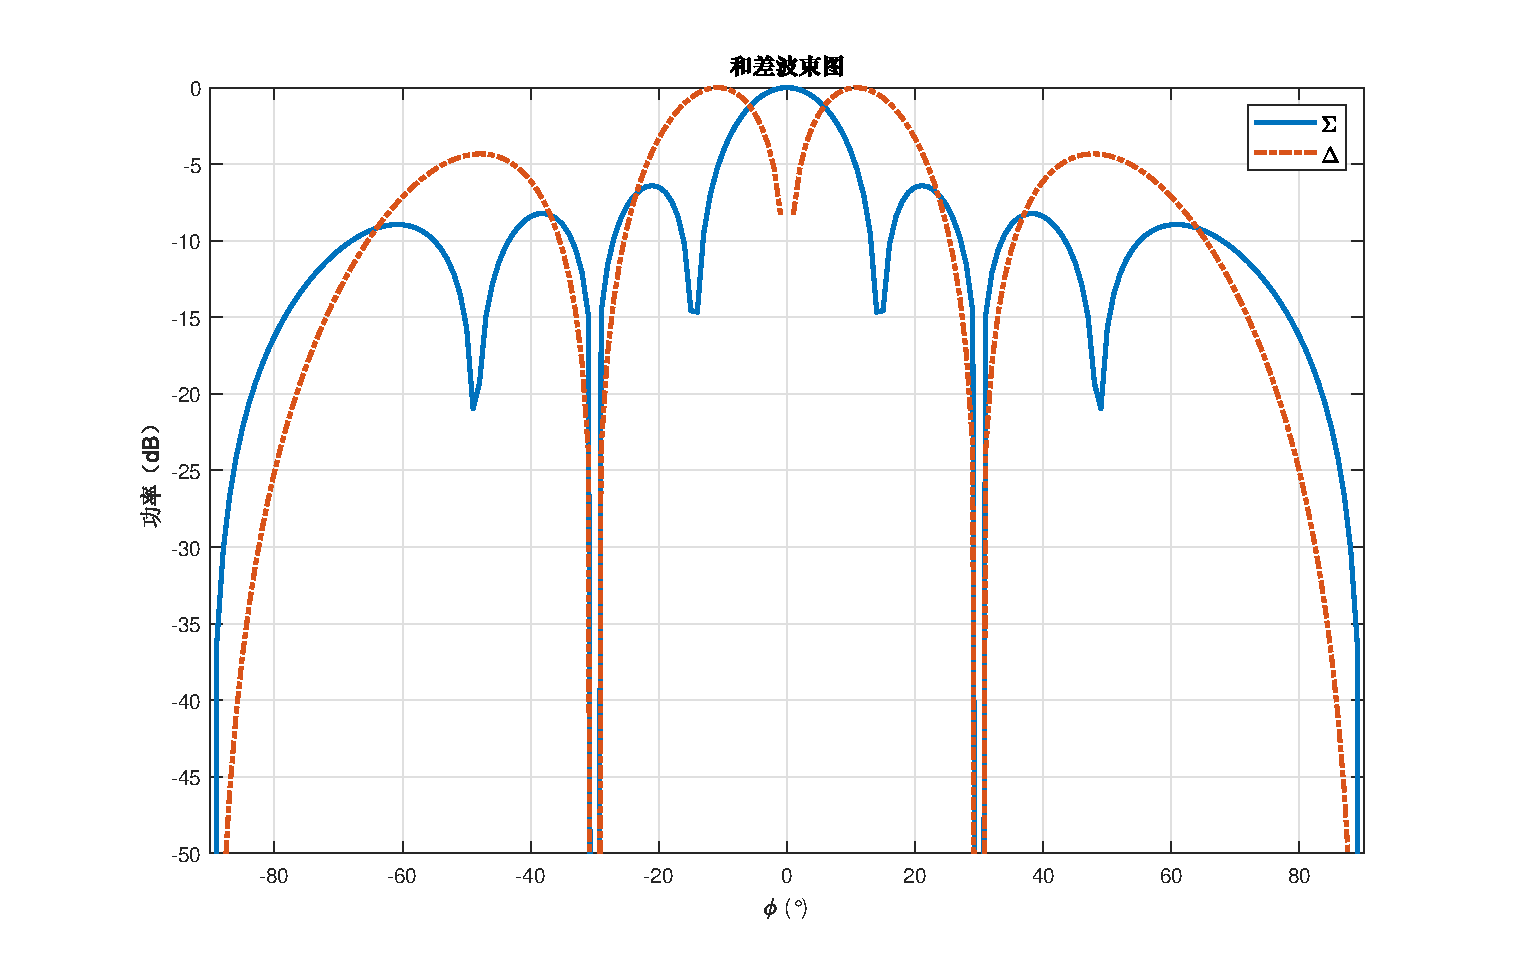
\includegraphics[scale=0.4]{pic/semi_sigma_delta.eps}
\caption{半阵法的和波束$\Sigma$与差波束$\Delta$}
\label{semi_sigma_delta}
\end{figure}

\begin{figure}[h]
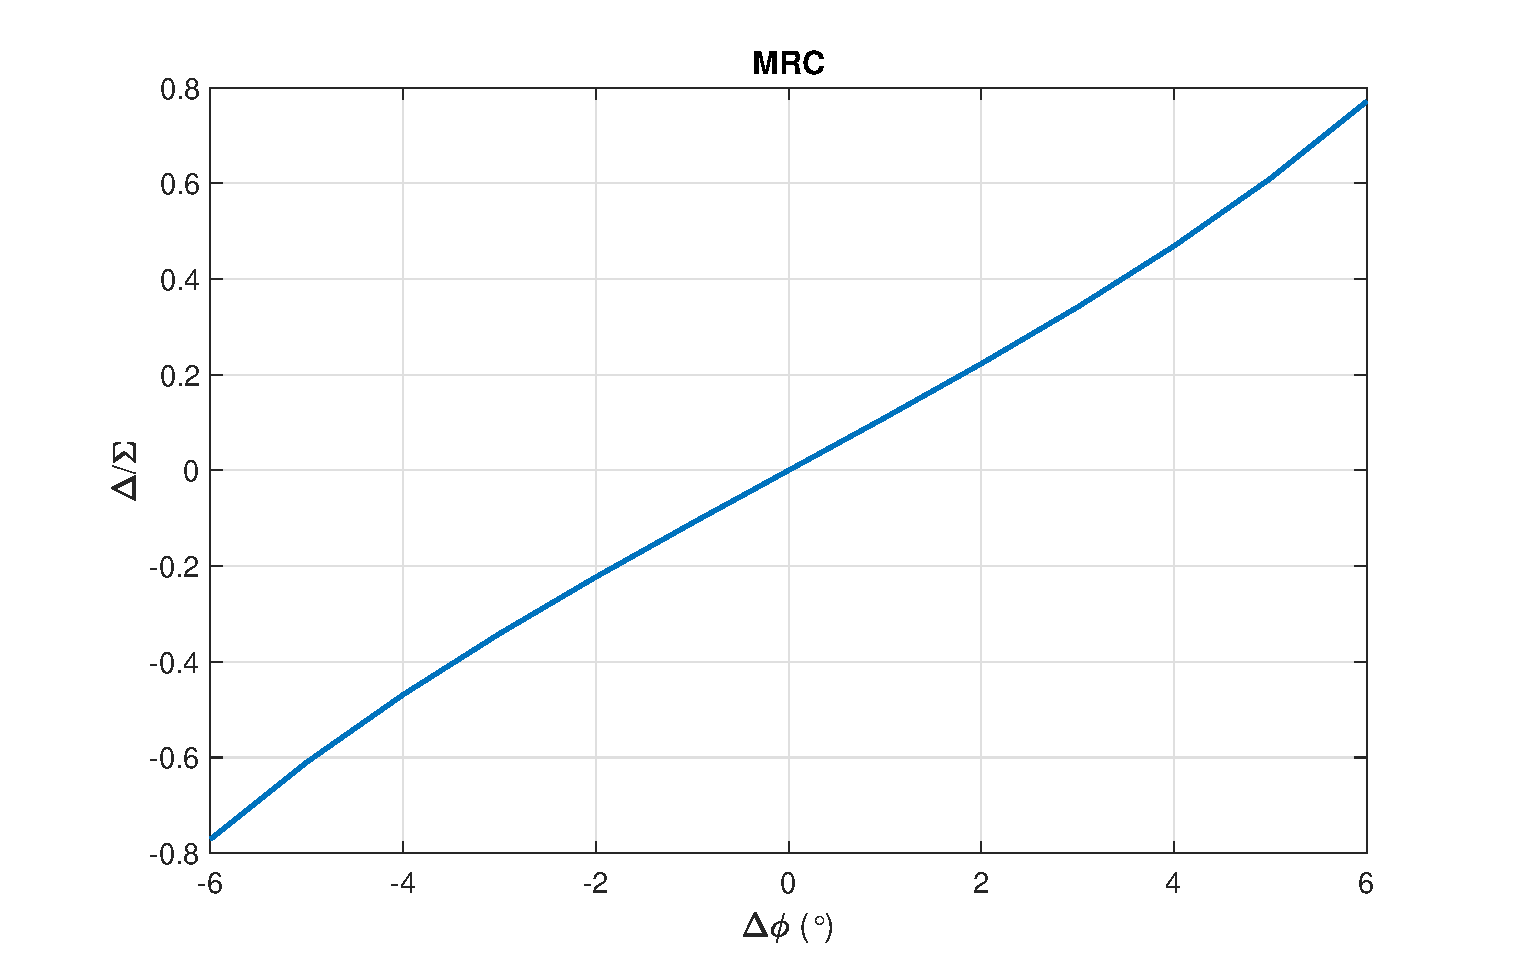
\includegraphics[scale=0.4]{pic/semi_MRC.eps}
\caption{半阵法的单脉冲比曲线}
\label{semi_MRC_figure}
\end{figure}

从图\ref{semi_sigma_delta}中我们可以看出,和波束的主瓣对准了$\phi_0=0^\circ$,
$3$dB衰减边界大致位于$\pm6^\circ$处。差波束在波束指向$\phi_0$处形成了一个较深的零陷,
注意图\ref{semi_sigma_delta}截断了衰减$-50$dB以下的部分。

对于单脉冲曲线图\ref{semi_MRC_figure},我们可以得知当角度$\phi$与波束指向角$\phi_0$较为接近时,
MRC的线性度较好,而在远离波束指向的地方,MRC的线性度较差。
这意味着期望信号的真实方向$\phi_s$偏离波束指向$\phi_0$越多,该方法的测量误差也就越大。

\subsection{加权测向}
半阵法理论过程简明清晰,且MRC有显式的表达式,但其利用了阵列对称性,因此只能用于均匀线阵和均匀面阵。
并且半阵法和差波束权向量直接选取了波束指向的导向向量,因此旁瓣抑制比较低,当测向环境中出现强旁瓣干扰时,
可能会使得该方法失效。因此,另一种设计和差波束权的方式应运而生。

加权法通过对波束指向处的导向向量$\bm{a}(\phi_0)$进行加窗处理,从而设计出一种满足给定旁瓣抑制比的和差波束。
传统的和差波束窗分别是Taylor窗和Bayliss窗,在作者的原文中,
这两种窗分别由圆形孔径和线形孔径天线(模拟天线,非阵列)导出,
而在接下来的内容中,我们将其拓展到均匀线阵上。

首先考虑一个长度为$2a$质地均匀的线形天线孔径,取其中点为参考点$O$,并假设信号以角度$\phi$入射,
如图\ref{linear_aperture}所示。
\begin{figure}[h]
    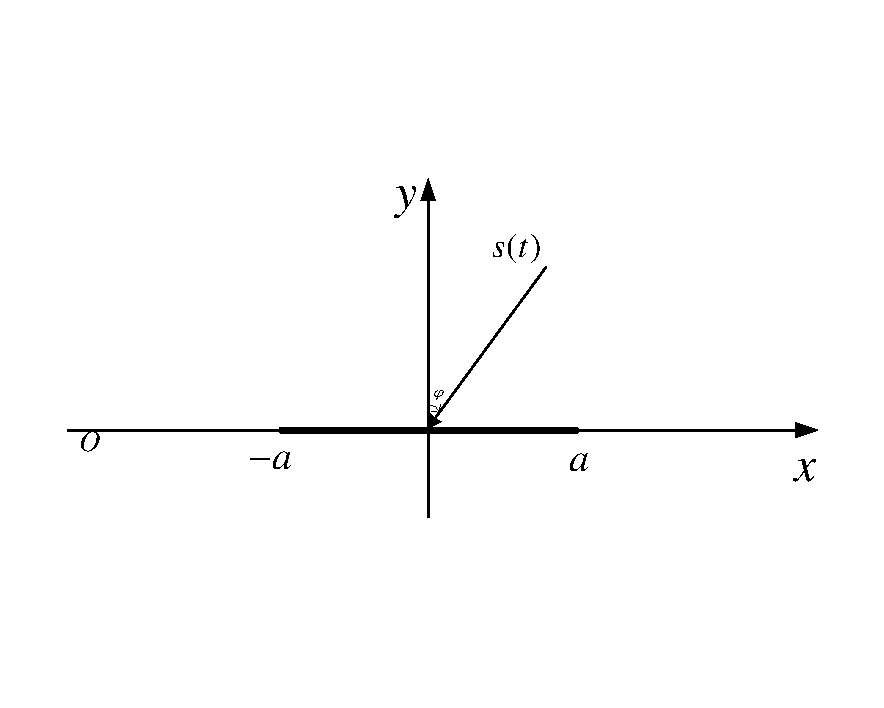
\includegraphics[scale=0.8]{pic/linear aperture.pdf}
    \caption{线性孔径接收信号模型}
    \label{linear_aperture}
\end{figure}

利用天线理论我们可以得知,线形孔径的响应函数$F(u)$为
\begin{equation}\label{aperture_response}
    \begin{aligned}
        F(u) = \int_{-\pi}^\pi g(x)e^{jux}dx
    \end{aligned}
\end{equation}
上式中,$g(x)$为孔径函数,即线形孔径上每个微元的单位冲激响应函数,
并且由
\begin{subequations}\label{ux_def}
    \begin{align}
        u &= \frac{2a}{\lambda}\sin\phi
        \\
        x &= \frac{\pi}{a}
    \end{align}
\end{subequations}
式\eqref{ux_def}中,$\lambda$为入射信号波长,
$2a$为线形孔径的长度,$\phi$为期望信号入射角度,如图\ref{linear_aperture}所示。
由于和波束要求响应函数为偶函数,因此我们将孔径函数$g(x)$以余弦级数展开得到式\eqref{cos_seq}。
\begin{equation}\label{cos_seq}
    \begin{aligned}
        g_{\Sigma}(x)=\left\{\begin{array}{ll}
        \sum\limits_{l=0}^{\bar{n}-1} B_{l} \cos \left(\mu_{l} x\right), & -\pi \leqslant x \leqslant \pi
        \\
        0, & \text { otherwise }
        \end{array}\right.
    \end{aligned}
\end{equation}
对于线形孔径,我们可以取$\mu_l=l$。
式\eqref{cos_seq}中,$\bar{n}$是我们期望抑制的邻近(主瓣)旁瓣个数。
我们定义对数旁瓣抑制比为$\text{SLL}$
\begin{equation}\label{SLL}
    \begin{aligned}
        \text{SLL} = 20\lg\eta = 10\lg\left(\nu_s^2/\nu_m^2\right)
    \end{aligned}
\end{equation}
式\eqref{SLL}中,$\nu_s^2$和$\nu_m^2$分别为旁瓣功率和主板功率。
在线形孔径的条件下,系数$B_l$由式\eqref{sigma_coeff}表出。
\begin{equation}\label{sigma_coeff}
    \begin{aligned}
        B_{m}=\left\{\begin{array}{ll}
        1, & m=0 \\
        (-1)^{m+1} \frac{\prod\limits_{n=1}^{\bar{n}-1} 1-\frac{m^{2}}{\sigma^{2}\left[A^{2}+(n-1 / 2)^{2}\right]}}{\prod\limits_{n=1 \atop n \neq m}^{\bar{n}-1} 1-\frac{m^{2}}{n^{2}}}, & 0<m<\bar{n} \\
        0, & m \geqslant \bar{n}
        \end{array}\right.
    \end{aligned}
\end{equation}
式\eqref{sigma_coeff}中,$A$和$\sigma^2$由式\eqref{A_sigma}表出。
\begin{subequations}\label{A_sigma}
    \begin{align}
        A &= \operatorname{acosh}\left(10^{-\mathrm{SLL} / 20}\right) / \pi \\
        \sigma^{2} &= \frac{\bar{n}^{2}}{A^{2}+(\bar{n}-1 / 2)^{2}}
    \end{align}
\end{subequations}
利用式\eqref{cos_seq}、\eqref{SLL}、\eqref{sigma_coeff}和\eqref{A_sigma}
我们就可以针对该线形孔径设计出符合要求的和波束权。

现在我们将该结论扩展到均匀线阵上。考虑一个$M$阵元的均匀线阵,阵元间距为半波长。
均匀线阵可以看作是对线形孔径的等间距采样,
此时阵列的输出由式\eqref{aperture_response}变为向量内积,即式\eqref{f_response}。
\begin{equation}\label{f_response}
    \begin{aligned}
        f(\phi) = \bm{g}_\Sigma^H\bm{a}(\phi)
    \end{aligned}
\end{equation}
上式中,$\bm{a}(\phi)$为导向向量,$\bm{g}_\Sigma$为Taylor幅度权向量。
由于均匀线阵是对线形孔径的等间距采样,因此我们可以得到$\bm{g}_\Sigma$的表达式
\begin{equation}\label{g_sigma_vec}
    \begin{aligned}
        \bm{g}_{\Sigma}=\left[g_{\Sigma}\left(x_{1}\right), g_{\Sigma}\left(x_{2}\right), \cdots,                     g_{\Sigma}\left(x_{M}\right)\right]^{T}
    \end{aligned}
\end{equation}
式\eqref{g_sigma_vec}中,$g_\Sigma(x)$为\eqref{cos_seq}中线形孔径函数$g(x)$的余弦展开式。
而$x_1,x_2,\cdots,x_M$表示在区间$\left[-\pi,\pi\right]$中均匀的取$M$个点,
由此得到$M$阵元均匀线阵的Taylor幅度权。

由于Taylor权向量$\bm{g}_\Sigma$为幅度权,不含有相位。因此我们可以通过式\eqref{taylor_w}
得到任意波束指向$\phi_0$的和波束权。
\begin{equation}\label{taylor_w}
    \begin{aligned}
        \bm{w}_\Sigma = \bm{g}_\Sigma \odot \bm{a}(\phi_0)
    \end{aligned}
\end{equation}
上式中,$\odot$表示Hadamard积。

接下来,我们讨论基于Bayliss幅度权的差波束权向量。
与Taylor权类似,均匀线阵的Bayliss权依旧可以从线形孔径模型下扩展得到。
同样,我们考虑一个长度为$2a$的线形孔径,取其中点为参考点$O$,入射信号波长为$\lambda$,角度为$\phi$,
如图\ref{linear_aperture}所示。其响应函数$F(u)$同式\eqref{aperture_response}。
由于差波束要求响应函数为奇函数,因此我们将孔径函数$g(x)$展开为正弦级数,如式\eqref{sin_seq}所示。
\begin{equation}\label{sin_seq}
    \begin{aligned}
        g_{\Delta}(x)=\left\{\begin{array}{ll}
        \sum\limits_{l=0}^{\bar{n}-1} B_{l} \sin \left(\mu_{l} x\right), 
        & -\pi \leqslant x \leqslant \pi \\
        0, & \text { otherwise }
        \end{array}\right.
    \end{aligned}
\end{equation}
对于线形孔径,我们可以取$\mu_l+1/2$。
同样的,我们定义旁瓣抑制比$\text{SLL}$,定义式同式\eqref{SLL},
以及期望约束的邻近(主瓣)旁瓣个数$\bar{n}$。
在线形孔径的条件下,系数$B_l$由式\eqref{delta_coeff}表出。
\begin{equation}\label{delta_coeff}
    \begin{aligned}
    B_{m}=\left\{\begin{array}{ll}
        \frac{C(-1)^{m}}{2 j}(m-1 / 2)^{2} \frac{\prod\limits_{n=1}^{\bar{n}-1} 
        1-\left(\frac{m+1 / 2}{\sigma Z_{n}}\right)^{2}}
        {\prod\limits_{n=1\atop n \neq m}^{n-1} 
        1-\left(\frac{m+1 / 2}{l+1 / 2}\right)^{2}}, & 0 \leqslant m \leqslant \bar{n}-1 \\
        0, & m>\bar{n}-1
        \end{array}\right.
    \end{aligned}
\end{equation}
上式中,$C$为常数,$\sigma$称为展宽因子,表达式为
\begin{equation}\label{delta_sigma}
    \begin{aligned}
       \sigma=\frac{\mu_{\bar{n}}}{Z_{\bar{n}}}=\frac{\bar{n}+1 / 2}{Z_{\bar{n}}}
    \end{aligned}
\end{equation}
而$Z_n$的定义则由式\eqref{Z_n}给出。
\begin{equation}\label{Z_n}
    \begin{aligned}
        Z_{n}=\left\{\begin{array}{ll}
                0, & n=0 \\
                \xi_{n}, & 0<n \leqslant 4 \\
                \sqrt{A^{2}+n^{2}}, & n>4
                \end{array}\right.
    \end{aligned}
\end{equation}
式\eqref{Z_n}中,$\xi_n$和$A$是与旁瓣抑制比SLL有关的常数,
可由表\ref{Z_n_coeff_tab}给出的SLL四阶多项式系数算出。
\begin{table}[h]
    \begin{tabular}{|c|c|c|c|c|c|}
    \hline
    \multirow{2}{*}{常量}  & \multicolumn{5}{|c|}{多项式系数}  \\
    \cline{2-6}
    & $C_0$ & $C_1$ & $C_2$ & $C_3$ & $C_4$ \\
    \cline{1-6}
    A & 0.30387530 & -0.05042922 & -0.00027989 & -0.00000343 & -0.00000002 \\
    \cline{1-6}
    $\xi_1$ & 0.98583020 & -0.03338850 & 0.00014064 & 0.00000190 & 0.00000001 \\
    \cline{1-6}
    $\xi_2$ & 2.00337487 & -0.01141548 & 0.00041590 & 0.00000373 & 0.00000001 \\
    \cline{1-6}
    $\xi_3$ & 3.00636321 & -0.00683394 & 0.00029281 & 0.00000161 & 0.00000000 \\
    \cline{1-6}
    $\xi_4$ & 4.00518423 & -0.00501795 & 0.00021735 & 0.00000088 & 0.00000000 \\
    \hline
    \end{tabular}
    \caption{$A$和$Z_n$的多项式系数}
    \label{Z_n_coeff_tab}
\end{table}

例如,$A$可以由式\eqref{A_deter}计算得出。
\begin{equation}\label{A_deter}
    \begin{aligned}
        A = C_0 + C_1\text{SLL} + C_2\text{SLL}^2 + C_3\text{SLL}^3 + C_4\text{SLL}^4
    \end{aligned}
\end{equation}
最后,利用式\eqref{sin_seq}、\eqref{delta_coeff}、\eqref{delta_sigma}和\eqref{Z_n}
并结合表\ref{Z_n_coeff_tab}即可设计出满足给定指标SLL和$\bar{n}$的线形孔径权。

均匀线阵的Bayliss权向量推到与Taylor权向量类似,我们依旧将均匀线阵看作是对线形孔径的等间距采样。
若假设均匀线阵有$M$个阵元,由式\eqref{g_sigma_vec}可以启发得到
\begin{equation}\label{g_delta_vec}
    \begin{aligned}
        \bm{g}_{\Delta}=\left[g_{\Delta}\left(x_{1}\right), 
        g_{\Delta}\left(x_{2}\right), \cdots, g_{\Delta}\left(x_{M}\right)\right]^{T}
    \end{aligned}
\end{equation}
式\eqref{g_delta_vec}中,$x_1,x_2,\cdots,x_M$是对区间$\left[-\pi,\pi\right]$均匀采样的$M$个点。
类似的,Bayliss权也是一个幅度权,不含有相位信息。
因此,任意波束指向$\phi_0$的Bayliss差波束权可以由式\eqref{bayliss_w}导出。
\begin{equation}\label{bayliss_w}
    \begin{aligned}
        \bm{w}_\Delta = \bm{g}_\Delta \odot \bm{a}(\phi)
    \end{aligned}
\end{equation}

至此,我们已经给出了均匀线阵的Taylor和波束权与Bayliss差波束权。
注意,本节中的公式以及结论仅使用于均匀线阵,若需将其拓展到均匀面阵和均匀圆阵,
可以查阅文献\cite{Taylor}和\cite{Bayliss},推导方法与本节类似。
接下来我们将以一个均匀线阵的例子来展示加权法的和差波束权以及单脉冲曲线。

考虑一个$8$阵元的均匀线阵,阵元间距为半波长。
我们取阵列波束指向$\phi_0=0^\circ$,旁瓣抑制比SLL为$-35$dB,抑制邻近旁瓣的个数$\bar{n}=4$。
Taylor权与Bayliss权形成的和差波束如图\ref{Taylor_Bayliss}所示。
\begin{figure}[h]
    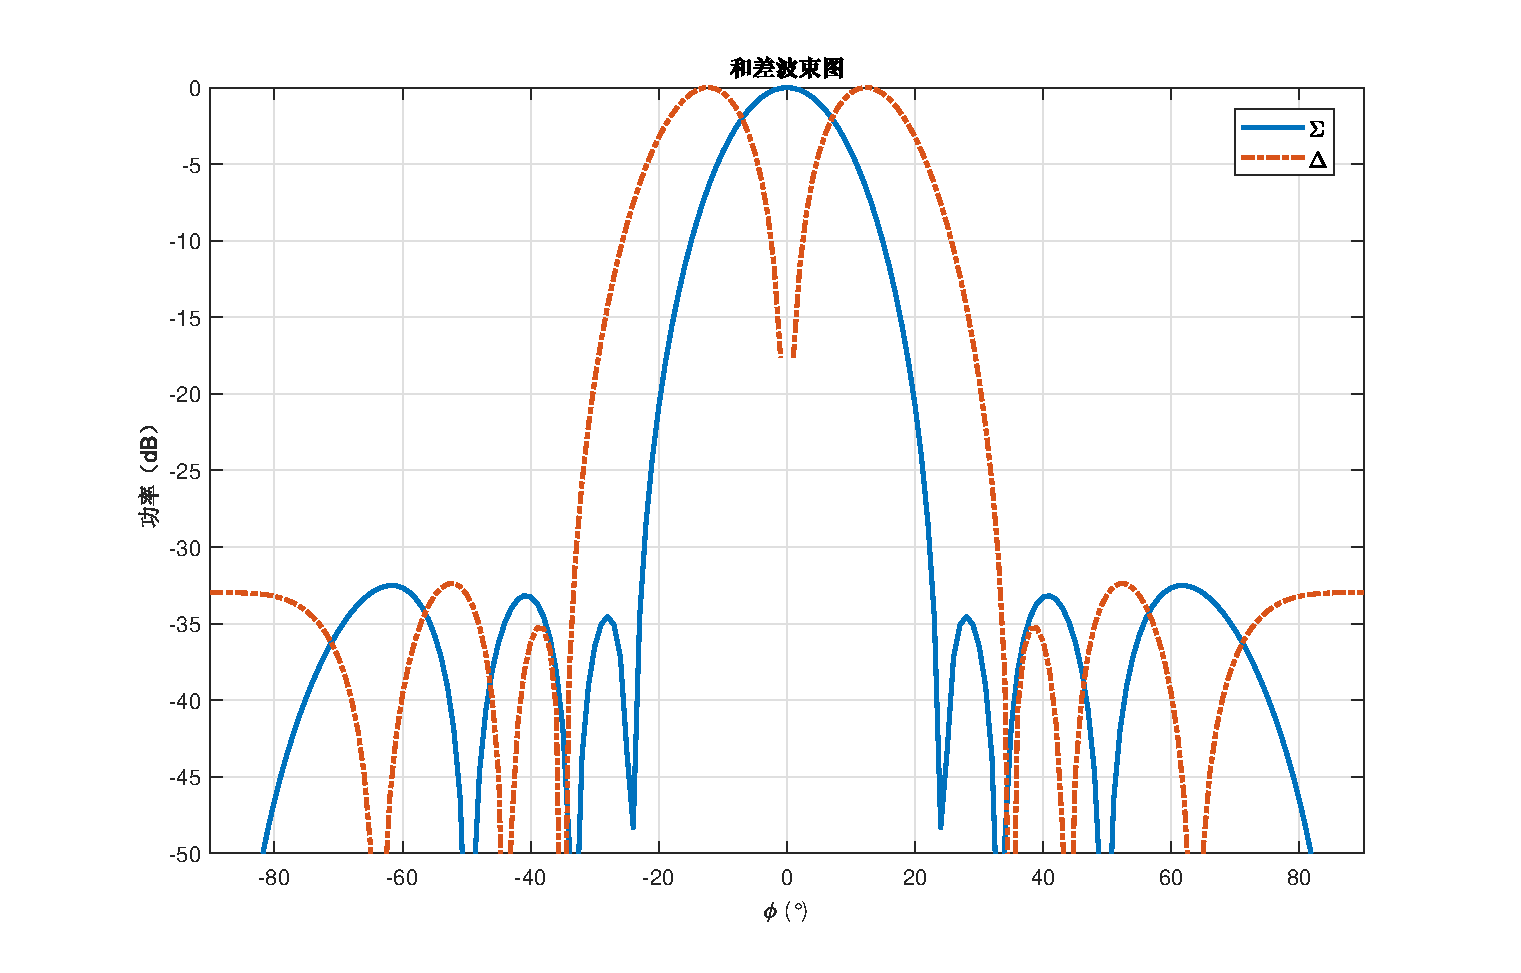
\includegraphics[scale=0.4]{pic/Taylor_Bayliss.eps}
    \caption{Taylor权形成的和波束$\Sigma$与Bayliss权形成的差波束$\Delta$}
    \label{Taylor_Bayliss}
\end{figure}

与半阵法的和差波束图\ref{semi_sigma_delta}相比,加权法得到的和差波束具有更低的旁瓣电平。
这意味着加权法具有更好的旁瓣抑制效果,能够应对存在旁瓣干扰的单脉冲测向场景。
但加窗的步骤使得主瓣展宽,和波束的3dB截止角度此时位于$\pm8^\circ$附近。
另外,加权法的单脉冲比MRC没有显式表达式,我们需要预先对MRC进行线性拟合才能够在单脉冲测向系统中使用它。
图\ref{Taylor_Bayliss_MRC}给出了加权法的单脉冲比曲线。
\begin{figure}[h]
    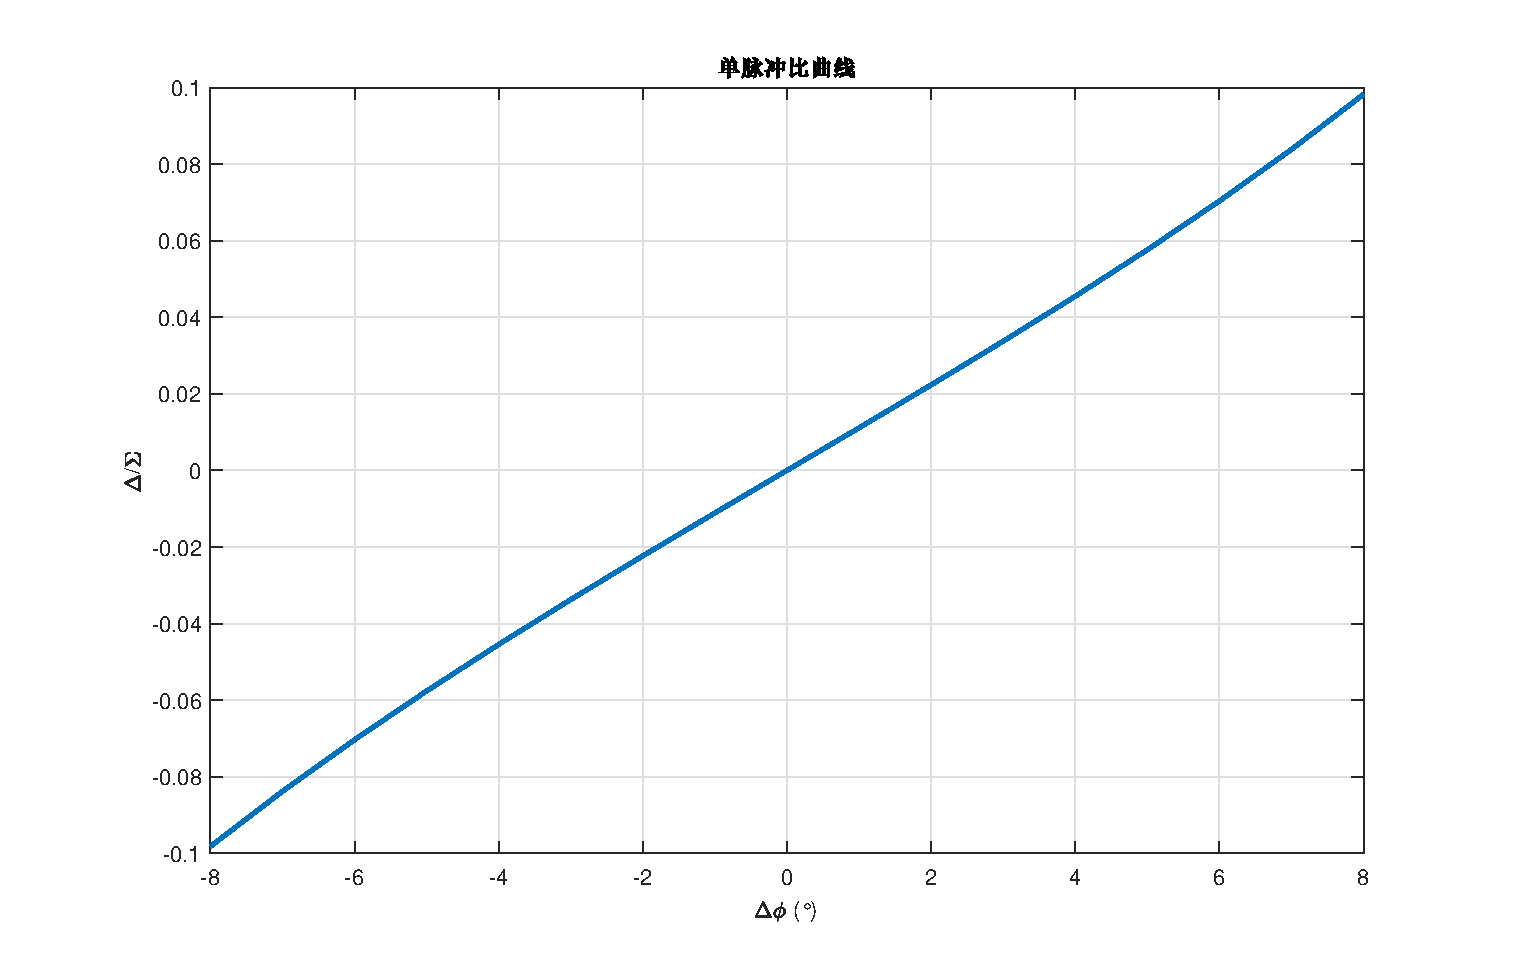
\includegraphics[scale=0.4]{pic/Taylor_Bayliss_MRC.eps}
    \caption{加权法的单脉冲比曲线}
    \label{Taylor_Bayliss_MRC}
\end{figure}

类似的,从图\ref{Taylor_Bayliss_MRC}中可以得知,在远离波束指向$\phi_0$时,MRC的线性度会下降,
从而使得此时的测角误差变大。

\subsection{和差比幅}
半阵法和加权法最大的局限性在于,它们都需要依赖于阵列的特殊结构。
前者要求阵列排布具有对称性,后者只能用于规则阵列且不具普适性,每种不同阵列的权向量表达形式可能会大相径庭。
而本节中将介绍一种名为和差比幅法的单脉冲测向方法。该方法的和差波束形成方式不依赖于阵列结构,
因此可以用于共形阵。

为简化问题,我们依旧以均匀线阵为例来解析和差比幅测向法的一般过程。
首先考虑一个$M$阵元的均匀线阵,阵元间距为半波长,期望信号波长为$\lambda$,阵列波束指向为$\phi_0$。
与半阵法类似,我们首先构造和波束权。由于和波束要求在波束指向处形成主瓣增益,因此我们取波束指向$\phi_0$
处的导向向量作为和波束权,即
\begin{equation}\label{ACM_w_s}
    \begin{aligned}
        \bm{w}_\Sigma = \bm{a}(\phi_0)
    \end{aligned}
\end{equation}
现在构造差波束权。由于差波束要求在波束指向处形成零陷,因此,一种可取的方法是:
首先以波束指向$\phi_0$为中心,关于$\phi_0$对称分别选取两个角度$\phi_l$和,$\phi_r$,
一般情况下,我们选择和波束主瓣的3dB截止角度作为$\phi_l$和$\phi_r$的值;
然后我们将差波束$\Delta(\phi)$构造为两个波束之差
\begin{equation}\label{ACM_delta}
    \begin{aligned}
        \Delta(\phi) = \left|\bm{a}^H(\phi_l)\bm{a}(\phi)\right| - 
                       \left|\bm{a}^H(\phi_r)\bm{a}(\phi)\right|
    \end{aligned}
\end{equation}
同理,比幅法也需要将和波束处理为幅度值,即式
\begin{equation}\label{ACM_sigma}
    \begin{aligned}
        \Sigma(\phi) = \left|\bm{w}_\Sigma^H\bm{a}(\phi)\right|
    \end{aligned}
\end{equation}
最后结合式\eqref{ACM_sigma}与\eqref{ACM_delta},得到比幅法的单脉冲比
\begin{equation}\label{ACM_MRC}
    \begin{aligned}
        \text{MRC} = \frac{\Delta(\phi)}{\Sigma(\phi)}
                   = \frac{ \left|\bm{a}^H(\phi_l)\bm{a}(\phi)\right| - 
                            \left|\bm{a}^H(\phi_r)\bm{a}(\phi)\right| }
                          { \left|\bm{w}_\Sigma^H\bm{a}(\phi)\right| }
    \end{aligned}
\end{equation}
从式\eqref{ACM_MRC}中可以看出,比幅测向顾名思义,是以差波束与和波束的幅度比作为单脉冲比,
实际上利用了左右波束的对称性,而不局限于阵列本身几何结构的特殊性,因此可以用于共形阵。
但该方法受阵列波束特性的影响,比如阵列的主瓣过宽时,可能会导致测向结果较差。
接下来我们仍然通过一个均匀线阵的例子来展示其特性。

考虑一个$8$阵元的均匀线阵,阵元间距为半波长,波束指向$\phi_0=0^\circ$,
我们取$\phi_l=-5^\circ$且$\phi_r=5^\circ$。
此时和差波束如图\ref{ACM_sigma_delta}所示。
\begin{figure}[h]
    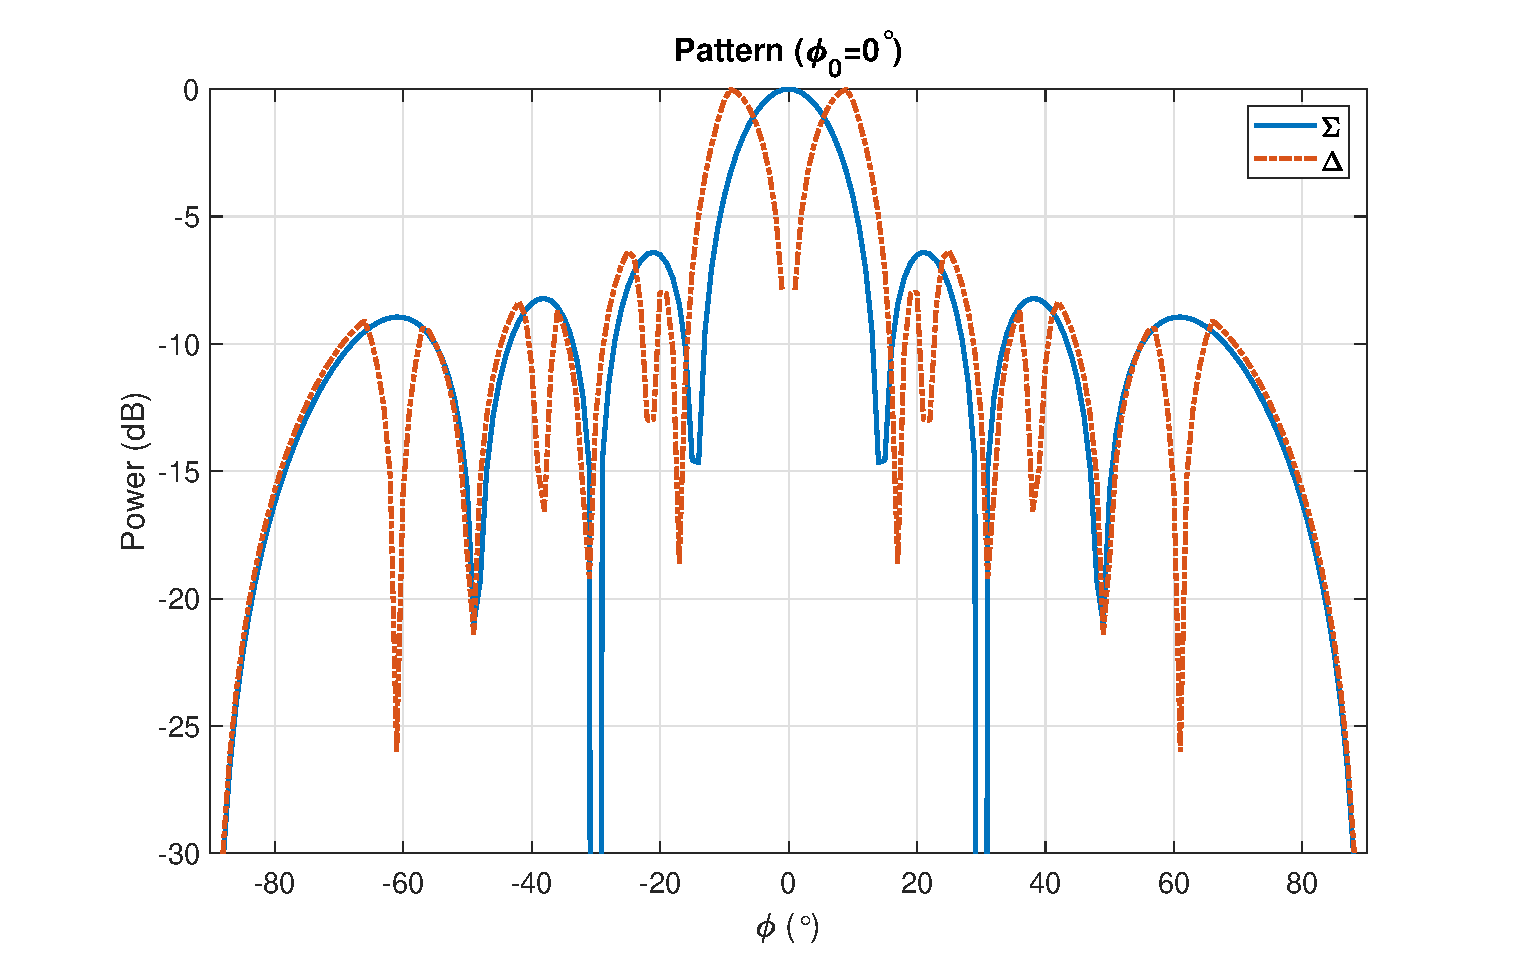
\includegraphics[scale=0.4]{pic/ACM_sigma_delta.eps}
    \caption{比幅法的和波束$\Sigma$与差波束$\Delta$}
    \label{ACM_sigma_delta}
\end{figure}

从图\ref{ACM_sigma_delta}中可以看出,与半阵法类似,比幅法的差波束依然在波束指向$\phi_0$处形成了零陷,
且旁瓣电平较高,难以抑制旁瓣干扰,仍旧无法用于存在强旁瓣干扰的场景。另外,比幅法的单脉冲比MRC也
不存在一个显式表达式,因此只能通过曲线拟合拟合出其斜率,然后在单脉冲测向系统中用于测向。
其单脉冲比曲线如图\ref{ACM_MRC_figure}所示。
\begin{figure}[h]
    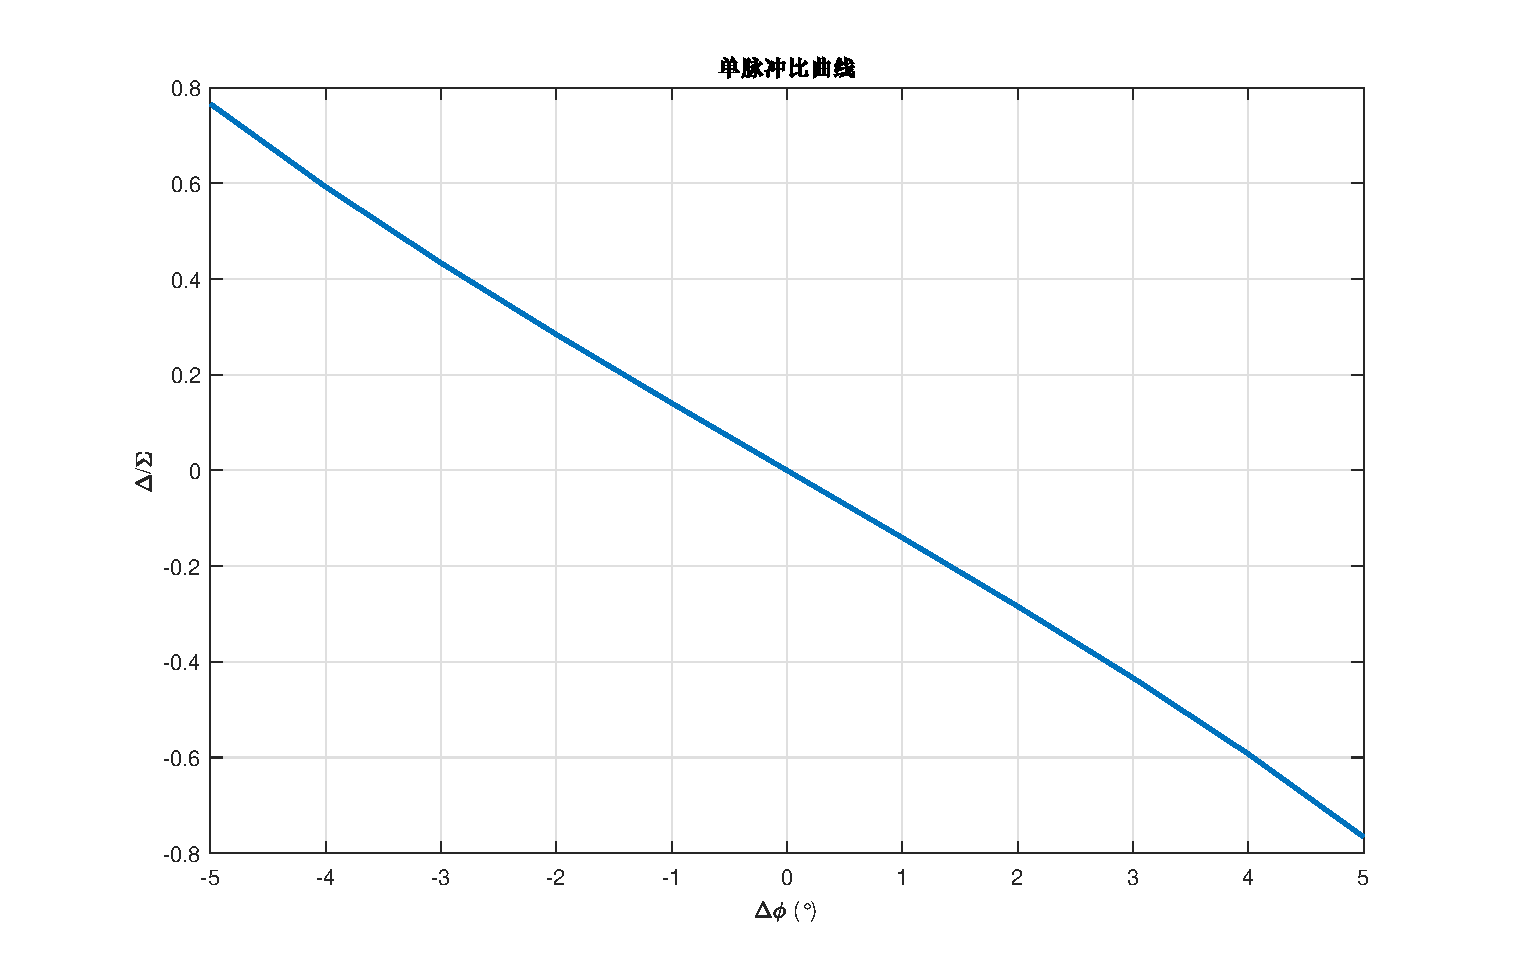
\includegraphics[scale=0.4]{pic/ACM_MRC.eps}
    \caption{比幅法的单脉冲比曲线}
    \label{ACM_MRC_figure}
\end{figure}

与之前的两种方法类似,MRC在远离波束指向角$\phi_0$时线性度会下降,进而影响测角精度。

\section{本章小结}
本章中,我们假设组成相控阵的所有阵元天线都是完全一致的全向天线,并给出了相控阵接收信号的数学模型,
进而简要的阐述了波束形成技术和传统单脉冲测向方法。

首先是相控阵的数学模型,依据阵元排布的方式,
我们将其划分为两大类,第一类是规则的阵列主要包含均匀线阵,均匀面阵和均匀圆阵。
我们通过几何光学计算出信号到达各个阵元的波程差,进一步给出其相位差,在远场窄带信号的假设下,
给出了这三种阵列的导向向量。第二类阵列是共形阵,主要特征为其“一般”性,即阵元排布不遵循某一特定规律。
在这种情况下,我们利用信号的方向余弦向量以及每个阵元的笛卡尔坐标计算出信号到达每个阵元的相位差,
进而给出一般导向向量表达式。值得注意的是,第一类规则阵列实际上是共形阵列的一种特殊形式,
其导向向量依然可以根据共形阵导向向量导出。

接着我们介绍了波束形成技术,阐述了波束形成的目的和一般手段。
然后介绍了两种波束形成方法,分别是MVDR方法和LCMV方法。
前者可以保证在设定的指向角$\phi_0$出形成主瓣增益,同时抑制干扰和噪声;
后者则可以在多个指向角同时形成波束和零陷,用于接收信号和抑制干扰。
实际上,MVDR方式是LCMV方法的一种特殊形式,即规定在指向角$\phi_0$处信号无失真通过。
在后续的章节中,我们还将利用LCMV结构进行单脉冲测向。

最后我们给出了三种常用的传统单脉冲测向方法,分别是半阵法、加权法和比幅法,
三种方法的优缺点各异。半阵法主要更近均匀线阵或均匀面阵的对称性,构造出和差波束权向量。
而在单脉冲测向问题中,期望信号的真实方向$\phi_s$往往接近于波束指向$\phi_0$,
因此半阵法利用该特性导出一个关于偏离角$\Delta\phi$的显式线性函数,进一步用于测向过程。
该方法简单易于实现,但依赖于阵列的几何结构,不能用于均匀圆阵和共形阵,
并且其和差波束的旁瓣电平都较高,无法应对有强旁瓣干扰存在时的场景。
因此,T. Taylor和E. T. Bayliss分别提出了一种和差波束加权方法,
进而设计出一种低旁瓣的和差波束权向量。该方法可以用于均匀线阵、均匀面阵和均匀圆阵,
其优点在于底旁瓣的波束能够在一定程度上抑制旁瓣干扰。但加窗的处理过程使得和波束主瓣有一定程度的展宽,
可能会造成测向精度下降,并且这种方法的单脉冲比没有显式表达式,因此只能先进行曲线拟合,
再将拟合好的数据用于后续的单脉冲测向过程。另外,该方法虽然可以拓展至均匀圆阵,
但仍旧无法将其用于共形阵。第三种方法是比幅测向法,该方法通过选取关于波束指向$\phi_0$对称的
两个角度的导向向量来构造差波束,并且单脉冲比直接用差波束与和波束的赋值进行比较,以此测量
偏离角$\Delta\phi$。该方法不受限于阵列结构,可以用于共形阵单脉冲测向。
但该方法与半阵法类似,和波束旁瓣电平仍然较高,无法应对强旁瓣干扰存在的场景。

\chapter{旁瓣干扰存在时的单脉冲测向方法}
在2.3节中,我们介绍了三种传统单脉冲测向方法,除去加权法以外,其余两种方法都无法应对旁瓣干扰。
在本章中,我们将介绍三类旁瓣干扰的抑制方法。第一类方法是波束优化方法,将低旁瓣的和差波束设计问题转化为一个优化问题,
然后求解该优化问题得出符合指标的和差波束权向量。第二类方法是遗传类算法,这类算法通过设计一个“个体适应度函数”,
用于筛选符合要求的解,进而得到一组低旁瓣和差波束权向量,以此抑制旁瓣干扰。第三类方法是广义旁瓣对象方法,
该方法利用辅助阵列阻塞期望信号,进而和主阵列的波束输出叠加,以此抵消旁瓣干扰。

\section{线性规划方法设计波束}
该方法由Rocca在2015年提出\cite{Rocca},主要针对均匀面阵或均匀线阵,利用阵列结构的对称性,构建线性规划问题,
设计低旁瓣的和差波束权向量。

\subsection{基本原理}
首先考虑一个$2M$行,$2N$列的均匀面阵,该阵列位于$xOy$平面,阵元个数为$2M\times2N$,组成阵列的天线均为完全一致的全向天线,
期望信号的波长为$\lambda$。那么,该阵列接收远场信号的波束输出$\text{AF}$可以表示为
\begin{equation}
    \begin{aligned}
        \text{AF}(u,v) = \sum_{m=1}^{2M}\sum_{n=1}^{2N}I_{mn}
        e^{j\frac{2\pi}{\lambda}\left[\left(m-M-1/2\right)d_xu+\left(n-N-1/2\right)d_yv\right]}
    \end{aligned}
\end{equation}
上式中,$u=\sin\phi\cos\theta$和$v=\sin\phi\sin\theta$表示入射信号的方向余弦,$d_x$和$d_y$分别表示$x$方向上的阵元间距
和$y$方向上的阵元间距。最重要的是,我们在这里定义的$I_{mn}=a_{mn}\exp(j\varphi_{mn})$表示第$m$行$n$列阵元的幅相因子。

显然,当波束指向为$(u_0,v_0)$时,相位因子
$$
\varphi_{mn}=-j2\pi/\lambda\left[\left(m-M-1/2\right)d_xu_0+\left(n-N-1/2\right)d_yv_0\right]
$$
即权为波束指向处的导向向量。为简化推导,我们假设此时波束指向$(u_0,v_0)=(0,0)$。由于和波束的幅度是关于波束指向偶对称的,
因此可以得到$a^\Sigma_{mn}=a^\Sigma_{(2M+1-m)n}=a^\Sigma_{m(2N+1-n)}=a^\Sigma_{(2M+1-m)(2N+1-n)}$。
这样我们就可以得到和波束的表达式,即式\eqref{lp_sigma_rep}。
\begin{equation}\label{lp_sigma_rep}
    \begin{aligned}
        \text{AF}^\Sigma(u,v) = 
        4\sum_{m=1}^{M}\sum_{n=1}^{N}a^\Sigma_{mn}
        \cos\left[\left(m-M-\frac{1}{2}\right)d_xu\right]\cos\left[\left(n-N-\frac{1}{2}\right)d_yv\right]
    \end{aligned}
\end{equation}
上式中,$a^\Sigma_{mn}$表示第$m$行$n$列阵元的幅度响应因子。而差波束响应是关于波束指向$(u_0,v_0)$偶对称的,
由此我们可以得到$a^\Delta_{mn}=a^\Delta_{(2M+1-m)n}=-a^\Delta_{m(2N+1-n)}=-a^\Delta_{(2M+1-m)(2N+1-n)}$,
同时负响应可以视作是给正响应施加了$\pi$的相移。因此,方位角通道和俯仰角通道的差波束响应如式\eqref{lp_delta_rep}所示。
\begin{subequations}\label{lp_delta_rep}
    \begin{align}
        \text{AF}^\Delta_{az}(u,v)&=
        4j\sum_{m=1}^M\sum_{n=1}^Na^\Delta_{mn}
        \sin\left[\left(m-M-\frac{1}{2}\right)d_xu\right]\cos\left[\left(n-N-\frac{1}{2}\right)d_yv\right] \\
        \text{AF}^\Delta_{el}(u,v)&=
        4j\sum_{m=1}^M\sum_{n=1}^Na^\Delta_{mn}
        \cos\left[\left(m-M-\frac{1}{2}\right)d_xu\right]\sin\left[\left(n-N-\frac{1}{2}\right)d_yv\right]
    \end{align}
\end{subequations}
根据文献\cite{Rocca},和波束幅度权的设计可以被表述为一个如下的凸优化问题
\begin{equation}\label{lp_sigma_opt}
    \begin{aligned}
        &\min_{\bm{a}_\Sigma} ~ -\text{AF}^\Sigma(u_0,v_0) \\
        &\text{s.t.} ~ \left|\text{AF}^\Sigma(u_s,v_s)\right|^2 \leqslant \text{UB}^\Sigma(u_s,v_s)
    \end{aligned}
\end{equation}
上式中,向量$\bm{a}^\Sigma$是由$a_{mn}^\Sigma$按列优先排成的向量,$\text{UB}^\Sigma(u_s,v_s)$是一个非负函数,
用于限定旁瓣的上界,而$(u_s,v_s),s=1,\cdots,S$表示旁边区域的方向余弦。同样,我们可以基于相同的原则,
得到差波束的凸优化问题,即
\begin{equation}\label{lp_delta_opt}
    \begin{aligned}
        &\min_{\bm{a}^\Delta} ~ -j\frac{\partial\text{AF}^\Delta_{az/el}(u,v)}{\partial w}|_{u=u_0,v=v_0} \\
        &\text{s.t.} ~ \text{AF}^\Delta_{az/el}(u_0,v_0) = 0, 
        \left|\text{AF}^\Delta_{az/el}(u_s,v_s)\right|^2 \leqslant \text{UB}^\Delta_{az/el}(u_s,v_s)
    \end{aligned}
\end{equation}
类似的,上式中的向量$\bm{a}^\Delta$是由$a_{mn}^\Sigma$按列优先排成的向量,下标$(\cdot)_{az/el}$表示方位角通道或者俯仰角通道。
变量$w$表示对方向余弦$u$或$v$求偏导数。$\text{UB}^\Delta_{az/el}(u_s,v_s)$是一个非负函数,用于限定差波束的上界。

由式\eqref{lp_sigma_rep}和\eqref{lp_delta_rep}可知,幅度因子是纯实数或纯虚数,因此式\eqref{lp_sigma_opt}
和\eqref{lp_delta_opt}中的二次约束条件可以被改写为式\eqref{lp_linear_constraint}。
\begin{subequations}\label{lp_linear_constraint}
    \begin{align}
        -\sqrt{\text{UB}^\Sigma(u_s,v_s)}\leqslant&\text{AF}^\Sigma(u_s,v_s)\leqslant\sqrt{\text{UB}^\Sigma(u_s,v_s)} \\
        -\sqrt{\text{UB}^\Delta_{az/el}(u_s,v_s)}\leqslant
        j&\text{AF}^\Delta_{az/el}(u_s,v_s)\leqslant\sqrt{\text{UB}^\Delta_{az/el}(u_s,v_s)}
    \end{align}
\end{subequations}
此时原凸优化问题就被简化为了一个线性规划问题。

现在,我们将和波束与差波束幅度权的优化问题合并为一个联合优化问题。从文献\cite{Rocca}中可以得知,和波束与差波束权可以共享某些元素,
即式\eqref{lp_identi_ele}。
\begin{equation}\label{lp_identi_ele}
    \begin{aligned}
        a^\Sigma_{mn} = a^\Delta_{mn}, ~ (m,n)\in\Psi
    \end{aligned}
\end{equation}
上式中,集合$\Psi$表示相同权向量元素的整数集。约束条件\eqref{lp_identi_ele}的引入减少了未知量的个数。
接着,我们导出和差波束幅度权向量的联合约束问题,优化目标为式\eqref{lp_joint_opt_obj}。
\begin{equation}\label{lp_joint_opt_obj}
    \begin{aligned}
        \min_{\bm{a}^\Delta} ~ -j\frac{\partial\text{AF}^\Delta_{az}(u,v)}{\partial u}|_{u=u_0,v=v_0} \\
    \end{aligned}
\end{equation}
约束条件为
\begin{subequations}\label{lp_joint_opt_const}
    \begin{center}
        \begin{equation}
            \text{AF}^\Delta_{az}(u_0,v_0) = 0
        \end{equation}
    \end{center}
    \begin{center}
        \begin{equation}
            -\text{AF}^\Sigma(u_0,v_0) \leqslant -\eta
        \end{equation}
    \end{center}
    \begin{center}
        \begin{equation}
            -\sqrt{\text{UB}^\Sigma(u_s,v_s)}\leqslant\text{AF}^\Sigma(u_s,v_s)\leqslant\sqrt{\text{UB}^\Sigma(u_s,v_s)}
        \end{equation}
    \end{center}
    \begin{center}
        \begin{equation}
            -\sqrt{\text{UB}^\Delta_{az}(u_s,v_s)}\leqslant
            j\text{AF}^\Delta_{az}(u_s,v_s)\leqslant\sqrt{\text{UB}^\Delta_{az}(u_s,v_s)}
        \end{equation}
    \end{center}
    \begin{center}
        \begin{equation}
            a^\Sigma_{mn} = a^\Delta_{mn}, ~ (m,n)\in\Psi
        \end{equation}
    \end{center}
\end{subequations}
\eqref{lp_joint_opt_const}式中,$\eta$是一个用户自定义的参数,用于约束和波束的幅度峰值。

由于以上过程中,我们得到的是和差波束的幅度权,因此与第二章中的加权法类似,
我们仍然可以利用波束指向处的导向向量$\bm{a}(\bm{\theta}_0)$来得到喝茶波束权,即式\eqref{lp_w_s_w_d}。
\begin{subequations}\label{lp_w_s_w_d}
    \begin{align}
        \bm{w}_\Sigma = \bm{a}_\Sigma \odot \bm{a}(\bm{\theta}_0) \\
        \bm{w}_\Delta^{az} = \bm{a}_\Delta^{az} \odot \bm{a}(\bm{\theta}_0) \\
        \bm{w}_\Delta^{el} = \bm{a}_\Delta^{el} \odot \bm{a}(\bm{\theta}_0) \\
    \end{align}
\end{subequations}
得到和差波束权向量后,即可得到方位角通道和俯仰角通道的单脉冲比,与加权法类似,由于我们是解优化问题得到的权向量,
因此没有固定的显式表达式,所以我们仍然需要曲线拟合来进行后续的单脉冲测向过程。

\subsection{仿真结果}

\section{差分进化算法设计低旁瓣差波束}
本节中,我们将介绍一种利用差分进化算法设计差波束的方法。该方法由Caorsi提出\cite{Caorsi}。
差分进化算法是遗传算法的一种改进形式,同样通过模拟种群的进化来求得符合要求的解。需要注意的是,
与遗传算法一样,差分进化算法也不保证得到全局最优解。本节中,我们以均匀线阵为例,给出该方法的一般过程,
并展示其数值仿真的结果。

\subsection{基本原理}
首先,考虑一个$M$阵元的均匀线阵,并且令$M=2N$,设入射信号的波长为$\lambda$,阵元间距为$d$。
此时均匀线阵的波束$F(\phi)$为
\begin{equation}\label{de_pattern_fromula}
    \begin{aligned}
        F(\phi) = \sum_{n=-N}^{-1}a_ne^{j\frac{2\pi}{\lambda}\left(n+1/2\right)d\sin\phi} +
        \sum_{n=1}^{N}a_ne^{j\frac{2\pi}{\lambda}\left(n-1/2\right)d\sin\phi}
    \end{aligned}
\end{equation}
上式中,$a_n$表示阵列中第$n$个阵元的幅度权,$\phi$表示信号俯仰角。

这里我们和上一节中一样,为简化推导过程设$\phi_0=0^\circ$。然后设和波束的幅度权为$a_n^\Sigma$,
由于和波束是关于波束指向$\phi_0$偶对称的,即$a_{-n}^{\Sigma}=a_{n}^{\Sigma}$。因此对于和波束,
式\eqref{de_pattern_fromula}缩减为
\begin{equation}\label{de_sigma_fromula}
    \begin{aligned}
        F_\Sigma(\phi) = 
        \sum_{n=1}^Na^\Sigma_{n}\cos\left[\frac{\pi}{\lambda}(2n-1)d\sin\phi\right]
    \end{aligned}
\end{equation}
式\eqref{de_sigma_fromula}为阵列和波束的表达式。然后我们将阵元划分为$P$个组,每个子阵的权值记为$g_p$,、
然后对组内成员进行优化,以求得满足条件的差波束。接着,我们用示性值$c_n$来表达阵元与组别的归属关系,
即当$c_n=p$时,表示阵元$n$属于第$p$个组,特别注意,当$c_n=0$时表示阵元$n$不纳入波束优化过程中。
第$p$个阵元组的集合由$\Gamma(p)$表示。
此时,第$n$个差波束的权值由式\eqref{de_delta_val}表出。
\begin{equation}\label{de_delta_val}
    \begin{aligned}
        a^\Delta_n = a^\Sigma_n\sum_{p=1}^{P}\delta_{c_np}g_p
    \end{aligned}
\end{equation}
上式中,$\delta_{c_np}$表示Kronecker函数,即当$c_n=p$时$\delta_{c_np}=1$,其余情况$\delta_{c_np}=0$。

此外,差波束是关于波束指向$\phi_0$奇对称的,即对于权值有$a^\Delta_{-n}=-a^\Delta_{n}$成立。
在这种情况下,差波束的表达式为
\begin{equation}
    \begin{aligned}
        F_\Delta(\phi) = 
        \sum_{n=1}^{N}a^\Delta_n\sin\left[\frac{\pi}{\lambda}(2n-1)d\sin\phi\right]
    \end{aligned}
\end{equation}
由于波束权值是对称的,因此只需要优化一半的权值即可,接下来我们给出衡量其好坏的代价函数。

在差分进化算法初始化的步骤中,我们要设置种群规模为$N_P$,它是随机生成的,随着种群的迭代而不断更新。
然后将$\bm{u}_k(i)$定义为第$k$次迭代中的第$i$个个体,其中$i=1,2,\cdots,N_P$。
在第$k$次迭代中,我们随机从种群中选出三个个体$\bm{u}_k(i_1)$,$\bm{u}_k(i_2)$和$\bm{u}_k(i_3)$,
用于产生第$k+1$次迭代的第$i$个个体,它们遵循如下原则
\begin{algorithm}[H]
    \KwData{$N_P$个个体$\bm{u}_0(1)\sim\bm{u}_0(N_P)$}
    \KwResult{完成$K$轮迭代后的最优个体$\bm{u}_K(i_{opt})$}
    初始化$\bm{u}_0(1)\sim\bm{u}_0(N_P)$为随机值\;
    \While{任意$f(\bm{u}_k(i))$不小于阈值$f_{th}$且$k<K$}{
        \begin{equation*}
            \begin{aligned}
                \bm{m}_k &= \left(\bm{u}_k(i_1)-\bm{u}_k(i_2)\right)F + \bm{u}_k(i_3) \\
                \tilde{\bm{u}}_{k+1}(i) &= \bm{m}_k \times \bm{u}_k(i)
            \end{aligned}
        \end{equation*}
        \eIf{$f(\tilde{\bm{u}}_{k+1}(i)) < f(\bm{u}_k(i))$}{
            $$
                \tilde{\bm{u}}_{k+1}(i) = \tilde{\bm{u}}_{k+1}(i)
            $$
        }{
            $$
                \tilde{\bm{u}}_{k+1}(i) = \bm{u}_{k}(i)
            $$
        }
    }
    \caption{差分进化算法}
    \label{de_algorithm_tab}
\end{algorithm}
表\ref{de_algorithm_tab}中,$\times$表示交叉操作,$F$是一个权值,而向量$\bm{m}_k$称为突变个体。$f(\cdot)$是代价函数,
用于评估个体的适应性。每轮迭代中,我们先用随机选出的三个个体产生突变个体$\bm{\mu}_k$,然后用突变个体与$\bm{u}_k(i)$交叉,
产生新个体$\tilde{\bm{u}}_{k+1}(i)$,若新个体的适应度高于原个体,则用它替代原个体,否则原个体不变,对于种群$N_P$中的所有个体,
都要做这样的操作,直到进入下一轮迭代。当有个体的代价小于阈值$f_{th}$或者达到最大迭代次数$K$时,算法终止。

对于该优化问题,向量$\bm{u}_k(i)$由两部分构成:一部分表示$P$组天线的权值;另一部分表示$N$长的天线。即
\begin{equation}
    \begin{aligned}
        \bm{u}_k(i) = \left[g_1,\cdots,g_P,c_1,\cdots,C_N\right]^T
    \end{aligned}
\end{equation}
另外,交叉操作$\times$的定义如下
\begin{equation}
    \begin{aligned}
        \bm{m} \times \bm{u} = \left[t_1, \cdots, t_{P+N}\right]^T
    \end{aligned}
\end{equation}
上式中,向量各个元素的定义由式\eqref{de_t_p}和\eqref{de_t_N}给出。
\begin{equation}\label{de_t_p}
    \begin{aligned}
        t_j = 
        \begin{cases}
            m_j, ~ \text{with probability} CR \\
            u_j, ~ \text{with probability} 1 - CR
        \end{cases}
    \end{aligned}
\end{equation}
上式中,$j=1,\cdots,P$。
\begin{equation}\label{de_t_N}
    \begin{aligned}
        t_j = 
        \begin{cases}
            \lfloor m_j+0.5 \rfloor, ~ \text{with probability} ~ CR \\
            \lfloor u_j+0.5 \rfloor, ~ \text{with probability} ~ 1 - CR
        \end{cases}
    \end{aligned}
\end{equation}
上式中,$j=P+1,\cdots,P+N$。
式\eqref{de_t_p}和\eqref{de_t_N}中,$m_j$和$u_j$分别表示向量$\bm{m}$和$\bm{u}$的第$j$个元素,
$\lfloor\cdot\rfloor$表示向下取整,$CR$为突变概率。

差分进化算法的关键在于突变概率$CR$和权值$F$的选择,选择不慎会造成差分进化算法的早熟,或是收敛速度较慢。
而它们的选择和具体的问题有关。在下一个子节中,我们选取一个均匀线阵的例子,展示他的性能。

\subsection{仿真结果}

\section{广义旁瓣对消方法}
与前两节中的波束设计方法不同,本节中将要介绍的广义旁瓣对消方法不是通过设计低旁瓣的和差波束权来抑制旁瓣干扰,
而是利用一个辅助阵列,阻塞期望信号,而使旁瓣干扰通过,进而在输出端与主阵列输出叠加,以此抵消旁瓣干扰。
本节中,我们将介绍广义旁瓣对消的一般原理,并针对均匀线阵给出一种阻塞矩阵的设计方法,最后展示其测向结果。

\subsection{广义旁瓣对消的基本原理}
旁瓣对消的基本流程如图\ref{GSC_process}所示。
\begin{figure}[h]
    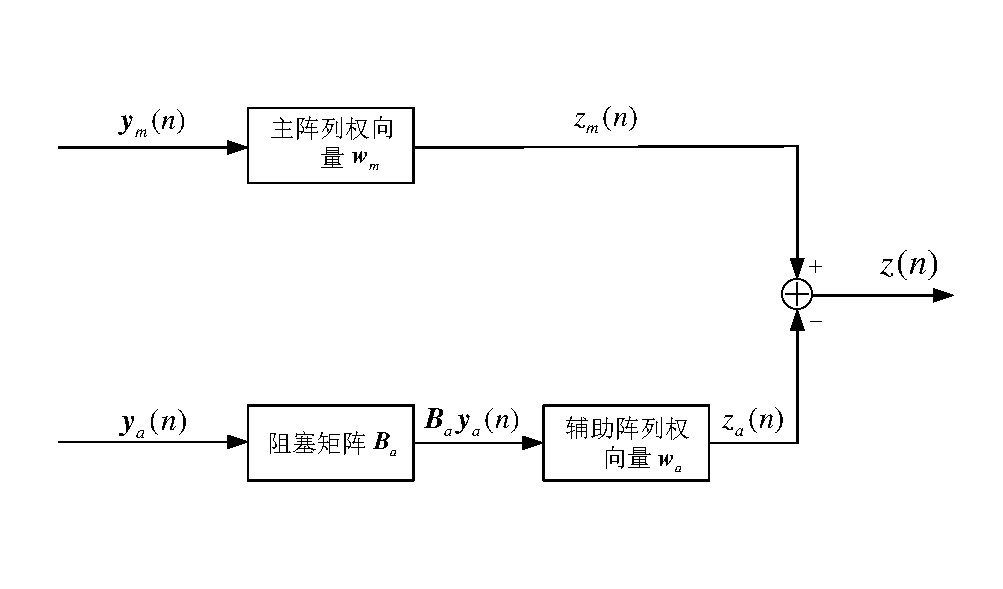
\includegraphics[scale=0.8]{pic/GSC_process.pdf}
    \caption{旁瓣对消流程示意图}
    \label{GSC_process}
\end{figure}
在图\ref{GSC_process}中,向量$\bm{y}_m$和$\bm{y}_a$分别是主阵列和辅助阵列的阵元接收信号。
辅助阵列接收信号$\bm{y}_a$通过阻塞矩阵$\bm{B}_a$后抑制期望信号$s(t)\bm{a}(\phi_s)$,
而旁瓣干扰保留进入辅助阵列的波束形成器,最后利用加法器$z_m(n)-z_a(n)$得到输出$z(n)$,
由于波束$z_m(n)$和$z_a(n)$中都含有旁瓣干扰,因此相互抵消,从而使得最终输出$z(n)$中不含有旁瓣干扰。
下面我们将以均匀线阵为例,阐述旁瓣对消的过程和一般原理。

首先考虑一个$M_m+M_a$阵元的均匀线阵,阵元间距为半波长,入射信号波长为$\lambda$,
主阵列为$M_m$阵元的子阵,辅助阵列为$M_a$阵元的子阵,并且它们的波束指向均为$\phi_0$。
我们设期望信号入射方向与波束指向相同,即$\phi_0=\phi_s$,
并且有$K$个旁瓣干扰信号,其角度分别为$\phi_1,\phi_2,\cdots,\phi_K$。
由式\eqref{data_model}可以得到主阵列的输出信号$z_m(n)$和辅助阵列输出信号$z_a(n)$
\begin{subequations}\label{gsc_data_model}
    \begin{align}
        \bm{y}_m(n) &= \bm{a}_m(\phi_0)s(n) + 
                       \sum_{k=1}^{K}\bm{a}_m(\phi_k)s_k(n) + \bm{n}_m
        \\
        \bm{y}_a(n) &= \bm{a}_a(\phi_0)s(n) + 
                       \sum_{k=1}^{K}\bm{a}_a(\phi_k)s_k(n) + \bm{n}_a
    \end{align}
\end{subequations}
为简化符号,我们设
\begin{subequations}\label{gsc_jamming}
    \begin{align}
        \bm{v}_m &= \sum_{k=1}^{K}\bm{a}_m(\phi_k)s_k(n) + \bm{n}_m
        \\
        \bm{v}_a &= \sum_{k=1}^{K}\bm{a}_a(\phi_k)s_k(n) + \bm{n}_a
    \end{align}
\end{subequations}
利用式\eqref{gsc_data_model}和式\eqref{gsc_jamming}结合图\ref{GSC_process}分别得到
旁瓣对消器的输出$z(n)$
\begin{equation}\label{gsc_z}
    \begin{aligned}
        z(n) &= z_m(n) - z_a(n)
        \\
             &= \bm{w}^H_m\bm{a}_m(\phi_0)s(n) + \bm{w}^H_m\bm{v}_m - z_a(n)
    \end{aligned}
\end{equation}
在式\eqref{gsc_z}中,旁瓣对消器要求辅助阵列输出$z_a(n)$不含有期望信号$s(n)$,
否则将会使得最终输出$z(n)$中的期望信号分量随着旁瓣干扰一并抵消。
因此,我们有必要设计一个阻塞矩阵$\bm{B}_a$,使得式\eqref{gsc_block}成立。
\begin{equation}\label{gsc_block}
    \begin{aligned}
        \bm{B}_a\bm{a}_a(\phi_0)s(n) = \textbf{0}
    \end{aligned}
\end{equation}
在第二节中,我们会介绍一种阻塞矩阵的设计方法。
为后续公式的导出,我们这里先假设式\eqref{gsc_block}成立,
此时辅助阵列的输出$z_a(n)$为
\begin{equation}\label{gsc_z_a}
    \begin{aligned}
        z_a(n) = \bm{w}_a^H\left(\bm{B}_a\bm{a}_a(\phi_0)s(n) + \bm{B}_a\bm{v}_a\right)
               = \bm{w}_a^H\bm{B}_a\bm{v}_a
    \end{aligned}
\end{equation}
将式\eqref{gsc_z_a}代入式\eqref{gsc_z}我们得到
\begin{equation}\label{gsc_out}
    \begin{aligned}
        z(n) = \bm{w}^H_m\bm{a}_m(\phi_0)s(n) + \bm{w}^H_m\bm{v}_m - \bm{w}_a^H\bm{B}_a\bm{v}_a
    \end{aligned}
\end{equation}
对于旁瓣对消器的输出$\bm{z}(n)$,我们需要使得其干扰叠加噪声分量最小,因此构造代价函数$J(\bm{w}_a)$
\begin{equation}\label{gsc_cost}
    \begin{aligned}
        J(\bm{w}_a) &= E\left\{\left|\bm{w}^H_m\bm{v}_m - \bm{w}^H_a\bm{B}_a\bm{v}_a\right|^2\right\}
        \\
                    &= \bm{w}_m^H\bm{Q}_{mm}\bm{w}_m - \bm{w}_m^H\bm{Q}_{ma}\bm{B}_a^H\bm{w}_a -
                       \bm{w}_a^H\bm{B}_a\bm{Q}_{am}\bm{w}_m +
                       \bm{w}_a^H\bm{B}_a\bm{Q}_{aa}\bm{B}_a^H\bm{w}_a
    \end{aligned}
\end{equation}
式\eqref{gsc_cost}中,矩阵$\bm{Q}_{mm}$和$\bm{Q}_{aa}$表示主阵列自相关和辅助阵列自相关矩阵,
矩阵$\bm{Q}_{am}$和$\bm{Q}_{ma}$表示主阵列与辅助阵列的互相关矩阵,其定义由式\eqref{gsc_cov_mat}给出。
\begin{subequations}\label{gsc_cov_mat}
    \begin{align}
        \bm{Q}_{mm} &= E\left\{\bm{v}_m\bm{v}_m^H\right\}
        \\
        \bm{Q}_{aa} &= E\left\{\bm{v}_a\bm{v}_a^H\right\}
        \\
        \bm{Q}_{am} &= E\left\{\bm{v}_a\bm{v}_m^H\right\}
        \\
        \bm{Q}_{ma} &= E\left\{\bm{v}_m\bm{v}_a^H\right\}
    \end{align}
\end{subequations}
对式\eqref{gsc_cost}中的代价函数$J(\bm{w}_a)$求梯度并令其等于零向量,
我们可以得到辅助阵列权向量$\bm{w}_a$的最优解
\begin{equation}\label{gsc_w_a}
    \begin{aligned}
        \bm{w}_a = \left(\bm{B}_a\bm{Q}_{aa}\bm{B}_a^H\right)^{-1}\bm{B}_a\bm{Q}_{am}\bm{w}_m
    \end{aligned}
\end{equation}
最后我们结合图\ref{GSC_process}与式\eqref{gsc_z}得到广义旁瓣对消器的输出$z(n)$。
\begin{equation}\label{gsc_fin_out}
    \begin{aligned}
        z(n) &= z_m(n) - z_a(n) \\
             &= \bm{w}^H_m\bm{y}_m(n) - \bm{w}^H_a\bm{y}_a(n) \\
             &= \bm{w}^H_m\bm{y}_m(n) - 
                \left(\bm{B}_a\bm{Q}_{aa}\bm{B}_a^H\right)^{-1}\bm{B}_a\bm{Q}_{am}\bm{w}_m\bm{y}_a(n)
    \end{aligned}
\end{equation}

注意,在整个推导过程中,我们假设主阵列权向量$\bm{w}_m$和阻塞矩阵$\bm{B}_a$都是已知的,
并且自相关和互相关矩阵也可以由各态历经性从时间平均中得出。阻塞矩阵$\bm{B}_a$的选取通常是不唯一的,
且对于不同的阵列,可能出现不同的结构,例如对于均匀线阵,其导向向量如式\eqref{sv_ULA},
一种可行的阻塞矩阵为式\eqref{simple_block}。
\begin{equation}\label{simple_block}
    \begin{aligned}
        \bm{B}_a = \begin{bmatrix}
                    \exp(j\varphi_0) & -1 & 0 & \cdots & 0 \\
                    0 & \exp(j\varphi_0) & -1 \cdots 0 \\
                    \vdots & \vdots & \ddots & \ddots & \vdots \\
                    0 & \cdots & 0 & \exp(j\varphi_0) & -1
                   \end{bmatrix}
    \end{aligned}
\end{equation}
上式中,$\varphi_0=2\pi d\sin\phi_0/\lambda$且$\bm{B}_a\in\mathbb{C}^{(M_a-1)\times M_a}$,
此时阻塞矩阵$\bm{B}_a$满足条件\eqref{gsc_block}。但我们注意到,辅助阵列的权向量$\bm{w}_a$
此时也被限定为一个$(M_a-1)\times1$的向量,即辅助阵列的自由度会将为$M_a-1$。
在随后的小节中,我们将介绍一种更为灵活的阻塞矩阵设计方式。

\subsection{一种基于准矩阵和SVD的阻塞矩阵设计方法}
本节我们将介绍一种灵活的阻塞矩阵设计方法,该方法Fernández等人15年提出\cite{Fernández}。
该方法巧妙的利用了准矩阵和SVD设计阻塞矩阵,在本节中,我们将以均匀线阵为例,给出该方法的一般过程。

首先考虑一个$M$阵元的均匀线阵,阵元间距为半波长,入射信号为远场窄带信号,波长为$\lambda$。
我们设窄带波束为$\bm{b}(s)$,其对应的波束形成权向量为$\bm{x}$,
由此可以得到式\eqref{block_beam_formula}。
\begin{equation}\label{block_beam_formula}
    \begin{aligned}
        \bm{F}(s)\bm{x} = \bm{b}(s)
    \end{aligned}
\end{equation}
上式中,$\bm{F}(s)$是$M$列的准矩阵,$\bm{b}(s)$是准向量。
准矩阵$\bm{F}(s)$的第$m$列是一个连续函数,如式\eqref{f_m}所示。
\begin{equation}\label{f_m}
    \begin{aligned}
        f_m(s) = \exp\left(j\pi(m-1)s\right)
    \end{aligned}
\end{equation}
式\eqref{f_m}中,$f_m$表示矩阵$\bm{F}(s)$的第$m$列,而$-1\le s \le 1$为一个连续变量,
表示阵列波束指向角的余弦值。而矩阵$\bm{F}(s)$的$k$行(作为准矩阵,实际上矩阵$\bm{F}(s)$有无穷多行)
是对应角度余弦值为$s_k$的导向向量,即
\begin{equation}\label{f_k}
    \begin{aligned}
        \bm{f}_k = \left[1, \exp\left(j\pi s_k\right), \exp\left(j\pi s_k\right), \cdots,
                   \exp\left(j\pi(M-1)s_k\right)
                   \right]
    \end{aligned}
\end{equation}
准向量$\bm{b}(s)$的结构类似,表示整个空域$s$的波束。

现在我们需要定义准向量的内积,考虑两个$[a,b] \times 1$维的准列向量$\bm{x}(s)$和$\bm{y}(s)$,
我们定义其内积为式\eqref{inner_prod}。
\begin{equation}\label{inner_prod}
    \begin{aligned}
        \bm{x}^H(s)\bm{y}(s) = \int_{a}^{b}x^*(s)y(s)ds
    \end{aligned}
\end{equation}
上式中,$\cdot^*$表示共轭。我们注意到,准矩阵$\bm{F}(s)$实际上是一个列酉形矩阵,
因此可以得到
\begin{equation}\label{F_unitary}
    \begin{aligned}
        \bm{F}^H(s)\bm{F}(s) = \bm{P}
    \end{aligned}
\end{equation}
式\eqref{F_unitary}中,矩阵$P$的第$m$行第$n$列元素定义为
\begin{equation}\label{P_mn}
    \begin{aligned}
        P_{m,n} = \int_{-1}^{1}\exp\left(j\pi s(n-m)\right)ds = 2\operatorname{sinc}(n-m)
    \end{aligned}
\end{equation}
结合式\eqref{F_unitary}和\eqref{P_mn}我们可以得到
\begin{equation}\label{P_iden}
    \begin{aligned}
        \bm{P} = \bm{F}^H(s)\bm{F}(s) = 2\bm{I}
    \end{aligned}
\end{equation}
利用式\eqref{P_iden}的结论,我们给准矩阵$\bm{F}(s)$的前面乘上一个系数$1/\sqrt{2}$,
使之归一化。现在准矩阵$\bm{F}(s)$满足列酉矩阵特性了,即$\bm{F}^H(s)\bm{F}(s) = \bm{I}$,
那么我们可以由式\eqref{block_beam_formula}及最小二乘法则构造优化问题
\begin{equation}\label{block_opt_obj}
    \begin{aligned}
        &\min_\bm{x} ~ \left(\bm{F}(s)\bm{x}-\bm{b}(s)\right)^H\left(\bm{F}(s)\bm{x}-\bm{b}(s)\right)
        \\
        &\text{s.t.} ~ \bm{x} = \bm{F}^H(s)\bm{b}(s)
    \end{aligned}
\end{equation}
式\eqref{block_opt_obj}中,向量$\bm{x}$的第$m$个元素由式\eqref{x_m}给出。
\begin{equation}\label{x_m}
    \begin{aligned}
        x_m &= \frac{1}{\sqrt{2}}\int_{-1}^{1}b(s)\exp\left(-j\pi s (m-1)\right)ds
        \\
            &= \frac{1}{\sqrt{2}}\mathcal{F}\left\{\bm{b}(s)\right\}|_{f=(m-1)/2}
    \end{aligned}
\end{equation}
上式中,$\mathcal{F}\left\{\cdot\right\}$表示傅里叶变换。

现在,我们考虑设计一个阻塞矩阵,其阻带为$s_a\le s \le s_b$,此时结合式\eqref{block_opt_obj},
我们可以构造出代价函数
\begin{equation}\label{block_cost}
    \begin{aligned}
        J(\bm{x},\bm{\mu}) = \left(\bm{F}(s)\bm{x}-\bm{b}(s)\right)^H\left(\bm{F}(s)\bm{x}-\bm{b}(s)\right)
                    -\bm{\mu}^H\left(\bm{G}\bm{x}-\bm{d}\right)
    \end{aligned}
\end{equation}
式\eqref{block_cost}中,$\bm{\mu}$表示$L$个元素的拉格朗日乘子,约束矩阵$\bm{G}$的第$l$行定义为
\begin{equation}
    \begin{aligned}
        \bm{g}_l = \frac{1}{\sqrt{2}}\left[1,\exp\left(j\pi s_l\right), 
                                           \exp\left(j\pi2 s_l\right), \cdots,
                                           \exp\left(j\pi(M-1)s_l\right)
                                      \right]
    \end{aligned}
\end{equation}
我们对式\eqref{block_cost}中的代价函数$J(\bm{x},\bm{\mu})$求梯度,并令其为零,
结合约束条件得到向量$\bm{x}$的解
\begin{equation}\label{x_solution}
    \begin{aligned}
        \bm{x} = \left(\bm{I}-\bm{G}^H(\bm{G}\bm{G}^H)^{-1}\bm{G}\right)\bm{F}^H(s)\bm{b}(s) + 
                 \bm{G}(\bm{G}\bm{G}^H)^{-1}\bm{d}
    \end{aligned}
\end{equation}
对于阵列的固有静态波束形成器,我们有
\begin{equation}\label{w_bf}
    \begin{aligned}
        \bm{b}(s) = \bm{F}(s)\bm{w}
    \end{aligned}
\end{equation}
成立,将式\eqref{w_bf}代入\eqref{x_solution},我们得到
\begin{equation}\label{x_solution_w}
    \begin{aligned}
        \bm{x} = \left(\bm{I}-\bm{G}^H(\bm{G}\bm{G}^H)^{-1}\bm{G}\right)\bm{w} + 
                 \bm{G}^H(\bm{G}\bm{G}^H)^{-1}\bm{d}
    \end{aligned}
\end{equation}
式\eqref{x_solution_w}中,向量$\bm{w}$是阵列的静态权,比如选取波束指向处的导向向量
$\bm{w}=\bm{a}(\phi_0)$或是第二章中介绍的Taylor权。现在,我们的目标转变为根据给定的要求,
构造约束矩阵$\bm{G}$和约束向量$\bm{d}$。

在本节中,我们的任务是构造一个满足要求的阻塞矩阵。因此,对于阻带$s_a\le s \le s_b$
我们可以令约束向量$\bm{d}=\textbf{0}$。
此时\eqref{x_solution_w}式被写为
\begin{equation}\label{x_without_d}
    \begin{aligned}
        \bm{x} = \left(\bm{I}-\bm{G}^H(\bm{G}\bm{G}^H)^{-1}\bm{G}\right)\bm{w}
    \end{aligned}
\end{equation}
为简化后续公式推导,可以定义投影矩阵$\bm{H}$
\begin{equation}\label{block_proj_mat}
    \begin{aligned}
        \bm{H} = \left(\bm{I}-\bm{G}^H(\bm{G}\bm{G}^H)^{-1}\bm{G}\right)
    \end{aligned}
\end{equation}
矩阵$\bm{H}$将向量$\bm{w}$投影到约束矩阵$\bm{G}$的零空间。

我们假设共有$L$点用于形成波束指向的阻带。然后对约束矩阵$\bm{G}$做SVD得到
\begin{equation}\label{G_SVD}
    \begin{aligned}
        \bm{G} = \bm{U}\bm{S}\bm{V}^H
    \end{aligned}
\end{equation}
式\eqref{G_SVD}中,矩阵$\bm{U}\in\mathbb{C}^{L\times L}$和$\bm{V}\in\mathbb{C}^{M\times M}$
都是酉矩阵,而矩阵$\bm{S}\in\mathbb{R}^{L\times M}_+$是一个拟对角矩阵,对角元为正奇异值和$0$,
且一般情况下,按递减排序。因此我们可以将矩阵$\bm{V}$分块得到
\begin{equation}\label{split_V}
    \begin{aligned}
        \bm{V} = \left[\bm{V}_1:\bm{V}_2\right]
    \end{aligned}
\end{equation}
式\eqref{split_V}中,波束指向个数一般小于阵元数即$L\le M$。此时式\eqref{block_proj_mat}可以改写为
\begin{equation}\label{block_proj_mat_V}
    \begin{aligned}
        \bm{H} = \bm{I} - \bm{V}_1\bm{V}_1^H = \bm{V}_2\bm{V}_2^H
    \end{aligned}
\end{equation}
然后利用准矩阵$\bm{G}(s)$的性质,我们构造一个矩阵$\bm{P}_G\in\mathbb{C}^{M\times M}$
\begin{equation}\label{P_G}
    \begin{aligned}
        \left[\bm{P}_G\right]_{m,n} &= \bm{G}^H(s)\bm{G}(s)
                                     = \frac{1}{2}\int_{s_a}^{s_b}\exp\left(j\pi(n-m)s\right)ds
        \\
                                    &= \frac{s_b-s_a}{2}\exp\left(j\pi(n-m)(s_a+s_b)/2\right)
                                       \operatorname{sinc}\left(\frac{(n-m)(s_b-s_a)}{2}\right)
    \end{aligned}
\end{equation}
式\eqref{P_G}中,$[\cdot]_{m,n}$表示矩阵的第$m$行第$n$列元素,
$s_a\le s \le s_b$为设计阻塞矩阵所要求的阻带。
我们可以进一步将式\eqref{P_G}改写为
\begin{equation}\label{P_G_fract}
    \begin{aligned}
        \bm{P}_G = \bm{D}\hat{\bm{P}}_G\bm{D}^H
    \end{aligned}
\end{equation}
上式中,矩阵$\bm{D}$是一个$M\times M$的对角酉矩阵,对角元为
\begin{equation}\label{mat_D}
    \begin{aligned}
        D_{m,m} = \exp\left(j\pi(m-1)s_c\right)
    \end{aligned}
\end{equation}
而半正定的Toeplitz矩阵$\hat{\bm{P}}_G$定义为
\begin{equation}\label{mat_P_G_hat}
    \begin{aligned}
         \left[\bm{P}_G\right]_{m,n}=\frac{W}{2} \operatorname{sinc}\left(\frac{(n-m) W}{2}\right)
    \end{aligned}
\end{equation}
式\eqref{mat_D}和\eqref{mat_P_G_hat}中,
\begin{subequations}
    \begin{align}
        s_c &= (s_a + s_b)/2
        \\
        W &= (s_b - s_a)
    \end{align}
\end{subequations}
上式中,$s_c$为阻带中心点,$W$为带宽。同样的,我们对矩阵$\bm{P}_G$做SVD并将式\eqref{G_SVD}代入得到
\begin{equation}\label{P_G_svd}
    \begin{aligned}
        \bm{P}_G = \bm{V}\bm{S}^H\bm{S}\bm{V}^H 
                 = \bm{D}\tilde{\bm{V}}\bm{S}^H\bm{S}\tilde{\bm{V}}^H\bm{D}^H
    \end{aligned}
\end{equation}
式\eqref{P_G_svd}中,$\tilde{\bm{V}}\bm{S}^H\bm{S}\tilde{\bm{V}}^H$
可以视作矩阵$\hat{\bm{P}}_G$的特征分解,且其特征值为实数。
由于$\hat{\bm{P}}_G$是一个缺秩矩阵,因为一般情况下$L \ll M$,所以我们可以取$\bm{S}$的前$L$个
大对角元构成矩阵$\bm{S}_L$将矩阵$\hat{\bm{P}}_G$近似为
\begin{equation}\label{P_G_hat_approx}
    \begin{aligned}
        \hat{\bm{P}}_G \approx \tilde{\bm{V}}_1\bm{S}_L^2\tilde{\bm{V}}_1^H
    \end{aligned}
\end{equation}
上式中,
\begin{equation}
    \begin{aligned}
        \tilde{\bm{V}} = \left[\tilde{\bm{V}}_1:\tilde{\bm{V}}_2\right]
    \end{aligned}
\end{equation}
因此我们得到
\begin{equation}\label{V1_reformula}
    \begin{aligned}
        \bm{V}_1 = \bm{D}\tilde{\bm{V}}_1
    \end{aligned}
\end{equation}
最后我们结合式\eqref{block_proj_mat_V}和\eqref{V1_reformula}得到投影矩阵
\begin{equation}\label{proj_mat_approx}
    \begin{aligned}
        \bm{H} = \bm{I} - \bm{D}\tilde{\bm{V}}_1\tilde{\bm{V}}_1^H\bm{D}^H
    \end{aligned}
\end{equation}
在给定阵列静态权$\bm{w}$的情况下,结合\eqref{x_without_d}和\eqref{block_proj_mat}
以及\eqref{proj_mat_approx}式即可得到在波束指向$\phi_0$处产生阻带的权向量。
在接下来的内容中,我们将以一个均匀线阵为例,展示该方法的阻塞矩阵效果。

考虑一个$16$阵元的均匀线阵,阵元间距为半波长,波束指向为$\phi_0=0^\circ$,
设定阻带为$-5^\circ$到$5^\circ$,对于式\eqref{P_G_hat_approx}中的近似,我们分别取$L=5$和$L=3$。
此时阻塞矩阵形成的波束$\Sigma_b$与波束指向导向向量形成的波束$\Sigma$如图\ref{GSC_Block_dif_L}所示。
\begin{figure}[h]
    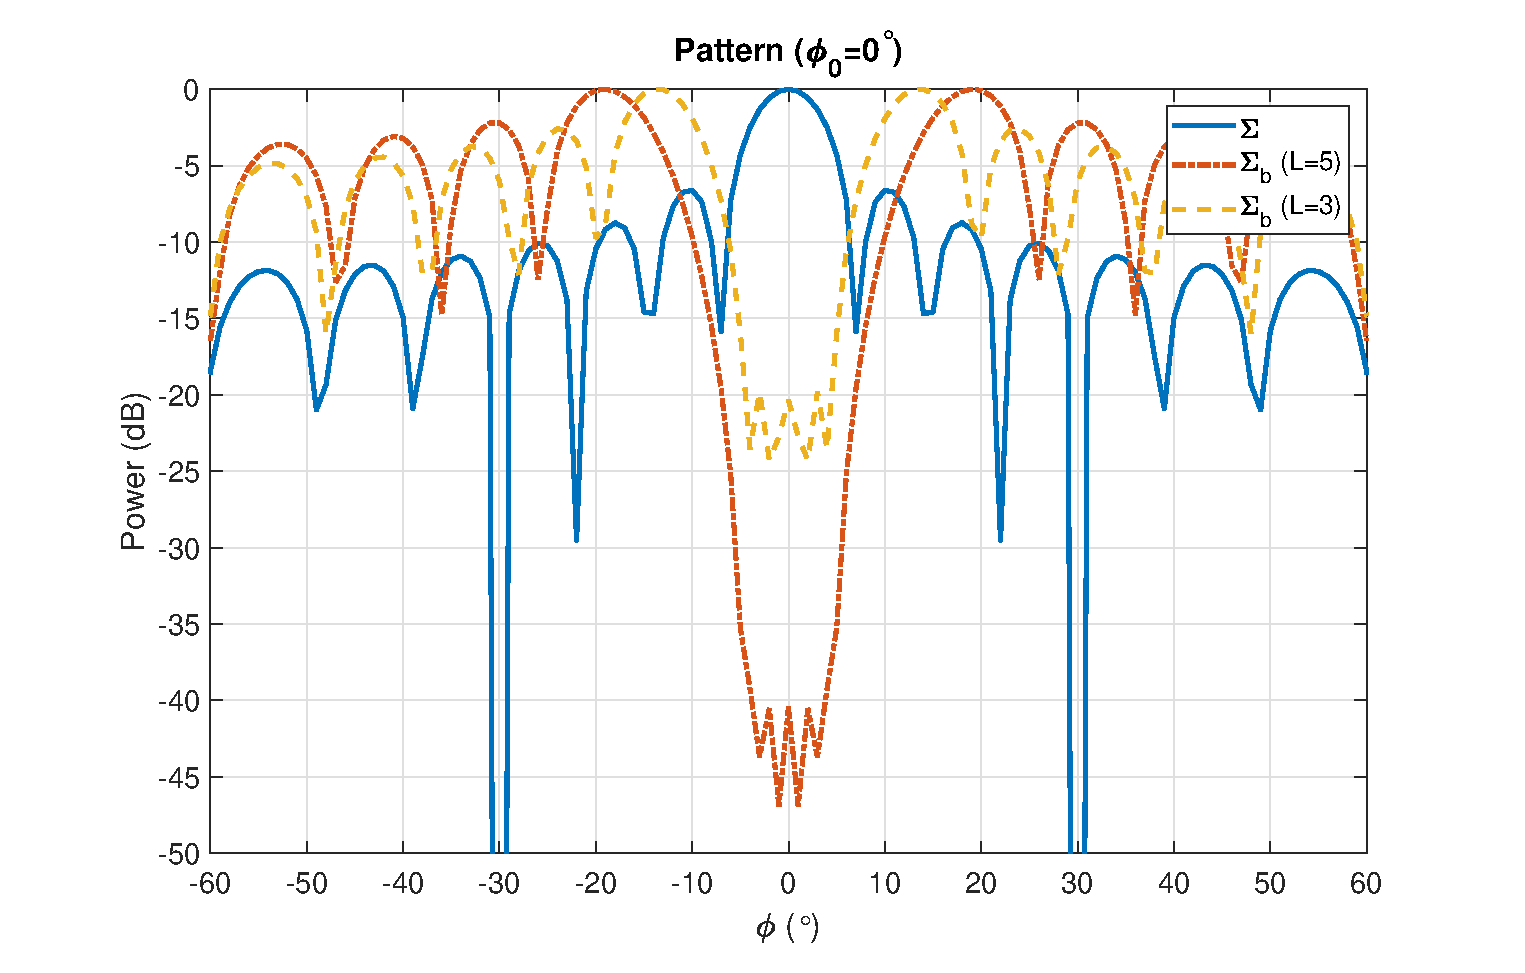
\includegraphics[scale=0.4]{pic/GSC_Block.eps}
    \caption{阻塞矩阵形成的波束$\Sigma_b$}
    \label{GSC_Block_dif_L}
\end{figure}

从图\ref{GSC_Block_dif_L}的结果中我们可以看出,该方法在$-5^\circ\le\phi\le5^\circ$处形成了阻带,
且阻塞效果,即主瓣抑制比随着近似点数$L$的增加而增大,也就是说$L$越大,设计的阻塞矩阵效果越好。

\subsection{均匀线阵旁瓣对消的仿真结果}

\section{本章小结}
本章中,我们讨论了三种应对旁瓣干扰的方法。前两种方法与传统单脉冲测向中的加权法类似,需要事先依照给定的技术指标,
设计出一套低旁瓣的静态和差波束权向量,通过既定的旁瓣抑制比来抑制旁瓣干扰。

第一种方法是线性规划方法设计和差波束权,该方法利用均匀面阵或均匀线阵的对称性,以及和波束的偶对称性与差波束的奇对称性,
将原凸优化问题种的二阶约束条件转变为一阶约束条件,并且遵循这样几个原则:第一,和波束在主瓣区域内需要满足一定的增益;
第二,差波束需要在波束指向处形成零陷;第三,差波束在波束指向处的斜率,即一阶导数要尽可能的大;
第四,和差波束的旁瓣功率都要尽可能的低。利用上述原则,将原本和差波束的两个优化问题转变为一个联合优化问题,
然后利用线性规划求解。

第二种方法是差分进化算法,该算法是一种遗传类算法,通过设计群体适应性函数,即代价函数,模拟自然选择和种群进化过程,
最终选取最后一轮进化的种群最优个体作为可行解。注意这里只给出了差波束设计方法,原文中的和波束使用的是Taylor权向量。
该方法与其他遗传算法类似,各类参数的选取非常重要,否则会出现早熟或是收敛速度过慢的问题。

第三种方法是广义旁瓣对消方法,该方法与上面两种静态方法不同,不再采用静态权向量,而是利用一个辅助阵列,
设计阻塞矩阵,使得期望信号通过辅助阵列时被阻塞,而旁瓣干扰可以无失真的通过,进而在主阵列和辅助阵列的输出端叠加二者,
使它们中的旁瓣干扰互相抵消,以此达到抑制旁瓣干扰的目的。在这个过程中,我们需要知道主阵列的自相关矩阵、辅助阵列的自相关矩阵
以及主阵列与辅助阵列的互相关矩阵。此外,我们还给出了一种阻塞矩阵的设计方法,它利用准矩阵和SVD,设计出满足阻带要求的阻塞矩阵
$\bm{B}_a$并用于辅助阵列。

线性规划和差分进化方法都是静态权向量方法,它们的优点在于静态权向量一经设计即可用于单脉冲测向系统,没有额外的在线计算过程。
但设计过程中的超参数过多,且影响较大,参数的选择不同,以及具体阵列的不同,都会影响静态权向量的设计结果。
广义旁瓣对消方法则是建立在已有的静态和差波束权向量之上(例如半阵法),利用辅助阵列以及干扰叠加噪声的三个相关矩阵,
在输出端叠加相消旁瓣干扰,是一种在线的旁瓣干扰抑制方法。一般情况下,辅助阵列的维度都小于主阵列,以此减小计算量。

\chapter{自适应单脉冲测向方法}
本章中,我们将介绍四类自适应单脉冲测向方法。第一节中介绍最大似然方法,它利用干扰叠加噪声的统计特性和似然函数,
结合牛顿公式给出了一种单脉冲测向方法。第二节中介绍MVAM方法,该方法假设一个理想的单脉冲比,
并在波束指向处做一阶泰勒展开,结合接收到的数据还原理想单脉冲比,以此给出一个单脉冲估计方法。
第三节中介绍正交置零方法,该方法利用方位角通道和俯仰角通道的可分离性,对主瓣干扰进行抑制,若想要抑制旁瓣干扰,
则还需与其余旁瓣干扰抑制方法结合使用,如加权法。第四节中介绍线性约束方法,该方法结合MVDR波束形成器,
约束波束指向以及测角区间边界点处的单脉冲比,使其成为关于偏离波束指向角$\Delta\theta$的线性函数,
然后借助LCMV结构,给出差波束权向量的最优解。并且在随后的小节中,我们给出了一种基于SVD的多点线性约束方法,
提升了原方法的测角精度,并尽可能的减少了阵列自由度的消耗。

\section{最大似然方法}
最大似然估计是一种自适应单脉冲测向方法,其核心在于利用已有的观测样本建立起似然函数$\mathcal{L}(\theta)$,
然后求该似然函数的最大解,得到待估计参数$\hat{\theta}=\operatorname{argmax}~\mathcal{L}(\theta)$。
U. Nickel 在 1993 年将该方法应用到了单脉冲系统中\cite{Nickel_93}。
该方法的优势在于,不受限于具体的阵列形式,只要能够知道干扰叠加噪声的统计特性,就可以利用该方法进行求解。

我们以一个$M$行$N$列的均匀面阵为例,分析该方法的导出过程。首先对于均匀面阵,我们可以利用式\eqref{data_model}和\eqref{sv_URA}
得到其接收信号模型
\begin{equation}\label{ML_data_model}
    \begin{aligned}
        \bm{y} = s(t)\bm{a}(\bm{\theta}) + \bm{n}
    \end{aligned}
\end{equation}
式\eqref{ML_data_model}中,复数$s(t)$表示期望信号的振幅,向量$\bm{\theta}=\left[\theta,\phi\right]^T$表示入射角度,
噪声向量$\bm{n}\in\mathbb{C}^{MN\times1}$表示
各阵元的噪声(或干扰叠加噪声)。若假设噪声向量服从复高斯分布$\bm{n}\sim\mathcal{CN}\left(0,\bm{Q}\right)$, 
则可知阵列接收数据的概率分布为$\bm{y}\sim\mathcal{CN}\left(s(t)\bm{a}(\bm{\theta}),\bm{Q}\right)$,
进一步我们可以得到其概率密度函数为式\eqref{pdf_y}。
\begin{equation}\label{pdf_y}
    \begin{aligned}
        p(\bm{y} \mid \bm{\theta}, s(t))=\pi^{-M}|\bm{Q}|^{-1} 
        \exp \left[-[\bm{y}-s(t) \bm{a}(\bm{\theta})]^{H} \bm{Q}^{-1}[\bm{y}-s(t) \bm{a}(\bm{\theta})]\right]
    \end{aligned}
\end{equation}
然后我们先对该密度函数取负对数似然,并去掉无关的常数部分,得到
\begin{equation}\label{lf_trans}
    \begin{aligned}
        S(\bm{\theta}, s(t))=-\mathcal{L}(\bm{\theta}, s(t))
        =[\bm{y}-s(t) \bm{a}(\bm{\theta})]^{H} \bm{Q}^{-1}[\bm{y}-s(t) \bm{a}(\bm{\theta})]
    \end{aligned}
\end{equation}
首先对上式中的参数$s(t)$求最小二乘解得到
\begin{equation}\label{least_square_s}
    \begin{aligned}
        s(t)=\left[\bm{a}^{H}(\bm{\theta}) \bm{Q}^{-1} \bm{a}(\bm{\theta})\right]^{-1} 
        \bm{a}^{H}(\bm{\theta}) \bm{Q}^{-1} \bm{y}
    \end{aligned}
\end{equation}
我们将式\eqref{least_square_s}带入\eqref{lf_trans}并去掉所有与参数$\bm{\theta}$无关的常数项得到其似然函数\eqref{lf}。
\begin{equation}\label{lf}
    \begin{aligned}
        S(\bm{\theta})=\bm{y}^{H} \bm{Q}^{-1} \bm{a}(\bm{\theta})
        \left[\bm{a}^{H}(\bm{\theta}) \bm{Q}^{-1} \bm{a}(\bm{\theta})\right]^{-1} 
        \bm{a}^{H}(\bm{\theta}) \bm{Q}^{-1} \bm{y}
    \end{aligned}
\end{equation}
为简化符号,定义$\bm{w}(\bm{\theta})$为自适应和波束权向量,由式\eqref{ml_w}表出。
\begin{equation}\label{ml_w}
    \begin{aligned}
        \bm{w}(\bm{\theta})=
        \left[\bm{a}^{H}(\bm{\theta}) \bm{Q}^{-1} \bm{a}(\bm{\theta})\right]^{-1 / 2} 
        \bm{Q}^{-1} \bm{a}(\bm{\theta})
    \end{aligned}
\end{equation}
将式\eqref{ml_w}代入\eqref{lf},我们可以将似然函数$S(\bm{\theta})$重写为
\begin{equation}
    \begin{aligned}
        S_{\mathrm{scan}}(\bm{\theta})=\left|\bm{w}^{H}(\bm{\theta}) \bm{y}\right|^{2}
    \end{aligned}
\end{equation}

接下来我们求解似然函数。为便于求解,我们令$F(\bm{\theta})=\ln \left[S_{\mathrm{scan}}(\bm{\theta})\right]$。
这样不改变似然函数的单调性,且期望信号方向的估计值$\hat{\bm{\theta}}$可以由式\eqref{ml_obj}给出。
\begin{equation}\label{ml_obj}
    \begin{aligned}
        \hat{\bm{\theta}}=\arg\max_{\bm{\theta}} F(\bm{\theta})
    \end{aligned}
\end{equation}
然后用牛顿梯度法给出对数似然函数$F(\bm{\theta})$的解,即式\eqref{newton_itr}。
\begin{equation}\label{newton_itr}
    \begin{aligned}
        \hat{\bm{\theta}}=\bm{\theta}_0-\bm{H}^{-1} \nabla F(\bm{\theta})
    \end{aligned}
\end{equation}
上式中,矩阵$\bm{H}=\nabla^2F(\bm{\theta})$是对数似然函数$F(\bm{\theta})$的海森矩阵。
在牛顿法中,还需要一个初值$\bm{\theta}_0$,幸运的是,单脉冲测向系统中恰好可以用阵列波束指向$\bm{\theta}_0$作为初值。

对于均匀面阵,其导向向量如式\eqref{subsv_URA}和\eqref{sv_URA}所示,为便于后续求导,我们可以将其改写为
\begin{equation}\label{URA_sv_uv}
    \begin{aligned}
        \left[\bm{a}(\bm{\theta})\right]_i = \exp\left[j\frac{2\pi}{\lambda}(x_iu+y_iv)\right]
    \end{aligned}
\end{equation}
式\eqref{URA_sv_uv}中,$x_i$和$y_i$表示第$i$个阵元(一般按列优先)的坐标,而参数$u$和$v$表示$x$和$y$方向上的方向余弦
\begin{subequations}\label{uv_def}
    \begin{align}
        u &= \sin\phi\cos\theta \\
        v &= \sin\phi\sin\theta
    \end{align}
\end{subequations}
注意,此处我们假设均匀面阵位于$xOy$平面,若位于坐标系其他平面,则方向余弦$u$和$v$及阵元坐标可能不一样。
现在,首先求对数似然函数关于的一阶偏导数,为简化符号,我们记一阶导数$F_u=\partial F/\partial u$。并且求导得
\begin{equation}\label{F_u}
    \begin{aligned}
        F_u &= \frac{(S_\mathrm{scan})_u}{S_\mathrm{scan}} \\
            &= \frac{\bm{w}^H_u\bm{y}\bm{y}^H\bm{w} + \bm{w}^H\bm{y}\bm{y}^H\bm{w}_u}{\bm{w}^H\bm{y}\bm{y}^H\bm{w}} \\
            &= 2\mathrm{Re}\left\{\frac{\bm{w}^H_u\bm{y}}{\bm{w}^H\bm{y}}\right\}
    \end{aligned}
\end{equation}
式\eqref{F_u}中,自适应和波束权向量$\bm{w}$的一阶导数$\bm{w}_u$定义如式\eqref{w_u}所示。
\begin{equation}\label{w_u}
    \begin{aligned}
        \bm{w}_{u} &=\left(\bm{a}^{H} \bm{Q}^{-1} \bm{a}\right)^{-1 / 2} 
        \bm{Q}^{-1} \bm{a}_{u}-\operatorname{Re}
        \left\{\bm{a}_{u}^{H} \bm{Q}^{-1} \bm{a} / 
        \bm{a}^{H} \bm{Q}^{-1} \bm{a}\right\} \bm{w} \\
        &=\bm{d}_{x}-\mu_{x} \bm{w}
    \end{aligned}
\end{equation}
上式中,
\begin{subequations}\label{dx_nd_mu}
    \begin{align}
        \bm{d}_{x}&=\left(\bm{a}^{H} \bm{Q}^{-1} \bm{a}\right)^{-1 / 2}\bm{Q}^{-1} \bm{a}_{u} \\
        \mu_x&=\operatorname{Re}\left\{\bm{a}_{u}^{H} \bm{Q}^{-1} \bm{a} / \bm{a}^{H} \bm{Q}^{-1} \bm{a}\right\}
    \end{align}
\end{subequations}
我们定义向量$\bm{d}_{x}$为自适应差波束权向量,并且对于均匀面阵我们有
\begin{equation}
    \begin{aligned}
        \left[\bm{a}_u\right]_i = j\frac{2\pi}{\lambda}x_i\exp\left[j\frac{2\pi}{\lambda}(x_iu+y_iv)\right]
    \end{aligned}
\end{equation}
最后将式\eqref{w_u}代入\eqref{F_u},得到一阶导数的最终表达式\eqref{F_u_fin}。
\begin{equation}\label{F_u_fin}
    \begin{aligned}
        F_u = 2\left(\operatorname{Re}\left\{\frac{\bm{d}_x^H\bm{y}}{\bm{w}^H\bm{y}}\right\}-\mu_x\right)
    \end{aligned}
\end{equation}
同理,我们可以得到对数似然函数$F(\bm{\theta})$关于$v$的一阶导数$F_v$,此处不做赘述。

接下来我们求解$F$的二阶导数$F_{uu}$。为简化后续计算,我们此处导出二阶导数$F_{uu}(\bm{\theta}_{max})$的近似值。
\begin{equation}\label{F_uu}
    \begin{aligned}
        F_{uu}(\bm{\theta}_{max}) &= 2\operatorname{Re}
        \left\{\frac{\bm{w}^H_{uu}\bm{y}\bm{w}^H\bm{y}-\bm{w}^H_u\bm{y}\bm{w}^H_u\bm{y}}
        {\left( \bm{w}^H\bm{y} \right)^2}\right\}(\bm{\theta}_{max}) \\
        &= 2\operatorname{Re}\left\{\frac{\bm{w}^H_{uu}\bm{y}}{\bm{w}^H\bm{y}}\right\}(\bm{\theta}_{max}) - 
           2\operatorname{Re}\left\{\left(\frac{\bm{w}^H_{u}\bm{y}}{\bm{w}^H\bm{y}}\right)^2\right\}(\bm{\theta}_{max})
           \\
        &= 2\operatorname{Re}\left\{\frac{\bm{w}^H_{uu}\bm{y}\bm{y}^H\bm{w}}
                                    {\bm{w}^H\bm{y}\bm{y}^H\bm{w}}\right\}(\bm{\theta}_{max}) - 
           2\operatorname{Re}\left\{\left(\frac{\bm{w}^H_{u}\bm{y}\bm{y}^H\bm{w}}
                                    {\bm{w}^H\bm{y}\bm{y}^H\bm{w}}\right)^2\right\}(\bm{\theta}_{max})
    \end{aligned}
\end{equation}
式\eqref{F_uu}中的第二项可以被改写为式\eqref{F_uu_2nd_term}。
\begin{equation}\label{F_uu_2nd_term}
    \begin{aligned}
        \operatorname{Re}\left\{\left(\frac{\bm{w}^H_{u}\bm{y}\bm{y}^H\bm{w}}
                                {\bm{w}^H\bm{y}\bm{y}^H\bm{w}}\right)^2\right\}(\bm{\theta}_{max})
        = \frac{1}{\left(\bm{w}^H\bm{y}\bm{y}^H\bm{w}\right)^2}
          \left(\operatorname{Re}^2\left\{\bm{w}^H_{u}\bm{y}\bm{y}^H\bm{w}\right\}-
          \operatorname{Im}^2\left\{\bm{w}^H_{u}\bm{y}\bm{y}^H\bm{w}\right\}\right)
    \end{aligned}
\end{equation}
首先,我们可以得到$\operatorname{Re}\left\{\bm{w}^H_{u}\bm{y}\bm{y}^H\bm{w}\right\}=0$,因为在最大值$\bm{\theta}_{max}$处,
一阶导数$F_u(\bm{\theta}_{max})=0$。其次,对于具有对称性的阵列,
有$\operatorname{Im}\left\{\bm{w}^H_{u}\bm{y}\bm{y}^H\bm{w}\right\}=0$成立,详情可见文献\cite{Nickel_93}。
这样式\eqref{F_uu}中只剩下了第一项
$2\operatorname{Re}\left\{\bm{w}^H_{uu}\bm{y}\bm{y}^H\bm{w}/\bm{w}^H\bm{y}\bm{y}^H\bm{w}\right\}(\bm{\theta}_{max})$。

接下来,我们用数学期望$E\left\{\bm{z}\bm{z}^H\right\}$代替式\eqref{F_uu}中的$\bm{z}\bm{z}^H$。我们取
\begin{equation}\label{ml_cov_mat}
    \begin{aligned}
        E\left\{\bm{z}\bm{z}^H\right\} = \beta^2\bm{a}(\bm{\theta}_s)\bm{a}^H(\bm{\theta}_s) + \bm{Q}
    \end{aligned}
\end{equation}
式\eqref{ml_cov_mat}中,$\beta^2$为期望信号的功率,$\bm{\theta}_s$为期望信号的实际方向。
而对于最大似然估计器,参数$\bm{\theta}$的估计是渐进无偏的,因此我们可以认为
$\bm{a}(\bm{\theta}_s)\approx\bm{a}(\bm{\theta}_{max})$。并且结合\eqref{ml_w}式可知$\bm{w}^H\bm{Q}\bm{w}=1$。
因此可以将式\eqref{F_uu}重写为式\eqref{F_uu_sim}。
\begin{equation}\label{F_uu_sim}
    \begin{aligned}
        F_{uu} &= 2\operatorname{Re}\left\{
            \frac
            {
                \beta^2\left(\bm{w}^H_{uu}\bm{a}+\bm{a}^H\bm{w}_{uu}\right)
                \left(\bm{a}^H\bm{Q}^{-1}\bm{a}\right)^{1/2} +
                \left(\bm{w}^H_{uu}\bm{a}+\bm{a}^H\bm{w}_{uu}\right)\left(\bm{a}^H\bm{Q}^{-1}\bm{a}\right)^{1/2}
            }
            {
                \beta^2\left(\bm{a}^H\bm{Q}^{-1}\bm{a}\right) + 1
            }
        \right\} \\
        &= \frac{\bm{w}^H_{uu}\bm{a}+\bm{a}^H\bm{w}_{uu}}{\left(\bm{a}^H\bm{Q}^{-1}\bm{a}\right)^{1/2}}
    \end{aligned}
\end{equation}
为了简化记号,我们省略上式及后文中的$\bm{\theta}_{max}$。利用条件$\bm{w}^H\bm{a}\bm{a}^H\bm{w}\approx0$
(同上文中式\eqref{F_uu_2nd_term}的化简),我们可以得到$\bm{d}^H_x\bm{a}=\mu_x\bm{w}^H\bm{a}$在$\bm{\theta}_{max}$
处成立,同理可得俯仰维$\bm{d}^H_y\bm{a}=\mu_y\bm{w}^H\bm{a}$。利用这些关系我们可以得到
\begin{subequations}\label{lf_2deri_trans}
    \begin{align}
        F_{uu} &= 2\operatorname{Re}^2
        \left\{
            \frac{\bm{a}^H_u\bm{Q}^{-1}\bm{a}}{\bm{a}^H\bm{Q}^{-1}\bm{a}}
        \right\} - 
        2\frac{\bm{a}^H_u\bm{Q}^{-1}\bm{a}_u}{\bm{a}^H\bm{Q}^{-1}\bm{a}} \\
        F_{vv} &= 2\operatorname{Re}^2
        \left\{
            \frac{\bm{a}^H_v\bm{Q}^{-1}\bm{a}}{\bm{a}^H\bm{Q}^{-1}\bm{a}}
        \right\} - 
        2\frac{\bm{a}^H_v\bm{Q}^{-1}\bm{a}_v}{\bm{a}^H\bm{Q}^{-1}\bm{a}} \\
        F_{uv} &= 2\operatorname{Re}
        \left\{
            \frac{\bm{a}^H_u\bm{Q}^{-1}\bm{a}}{\bm{a}^H\bm{Q}^{-1}\bm{a}}
        \right\}
        \operatorname{Re}
        \left\{
            \frac{\bm{a}^H_v\bm{Q}^{-1}\bm{a}}{\bm{a}^H\bm{Q}^{-1}\bm{a}}
        \right\} - 
        2\frac{\bm{a}^H_u\bm{Q}^{-1}\bm{a}_v}{\bm{a}^H\bm{Q}^{-1}\bm{a}}
    \end{align}
\end{subequations}

注意,式\eqref{lf_2deri_trans}中仍然省略了$\bm{\theta}_{max}$。在单脉冲测向系统中,
期望信号的真实方向$\bm{\theta}_s$往往处于波束指向$\bm{\theta}_0$的主瓣内,
这意味着$\bm{\theta}_s$和$\bm{\theta}_0$较为接近,而最大似然估计器是一个渐进无偏估计器,
我们可以认为$\bm{\theta}_{max}=\bm{\theta}_s$,因此可以取波束指向$\bm{\theta}_0$处的值代入式\eqref{lf_2deri_trans}
作为近似。结合式\eqref{dx_nd_mu}我们可以得到对数似然函数$F$的二阶导数。
\begin{subequations}\label{lf_2d}
    \begin{align}
        F_{uu} &= 2\mu^2_x - 2\frac{\bm{d}^H_x\bm{a}_u}{\bm{w}^H\bm{a}} \\
        F_{vv} &= 2\mu^2_v - 2\frac{\bm{d}^H_y\bm{a}_v}{\bm{w}^H\bm{a}} \\
        F_{uv} &= 2\mu_x\mu_y - 2\frac{\operatorname{Re}\left\{\bm{d}^H_x\bm{a}_v\right\}}{\bm{w}^H\bm{a}}
    \end{align}
\end{subequations}
式\eqref{lf_2d}中,各参数取波束指向$\bm{\theta}_0$处的值。

最后,我们可以利用式\eqref{lf_2d}构建海森矩阵$\bm{H}$。
\begin{equation}\label{hessian_mat}
    \begin{aligned}
        \bm{H} = 
        \begin{bmatrix}
            F_{uu} & F_{uv} \\
            F_{uv} & F_{vv}
        \end{bmatrix}
    \end{aligned}
\end{equation}
以及对数似然函数的梯度$\nabla F$,即雅可比矩阵
\begin{equation}\label{jacobian_mat}
    \begin{aligned}
        \nabla F = \left[F_{u},F_{v}\right]^T
    \end{aligned}
\end{equation}
结合牛顿公式\eqref{newton_itr}得到方向余弦的估计值$\hat{u}$和$\hat{v}$。
\begin{equation}
    \begin{aligned}
        \left[\hat{u},\hat{v}\right]^T = \left[u_0, v_0\right]^T - \bm{H}^{-1}(\bm{\theta}_0)\nabla F(\bm{\theta}_0)
    \end{aligned}
\end{equation}
最后利用反三角函数即可估计出期望信号的入射方向$\hat{\bm{\theta}}$。

\section{MVAM方法}
本节中,我们同样以$M$行$N$列的均匀面阵为例,解析MVAM方法的一般过程。
首先信号模型同式\eqref{ML_data_model}一样。我们设单脉冲比为$R$,而无噪声的理想单脉冲比为$R_0$。
它们由式\eqref{MVAM_MRC}给出。
\begin{equation}\label{MVAM_MRC}
    \begin{aligned}
        R &= \frac{\bm{w}^H_\Delta\bm{y}}{\bm{w}^H_\Sigma\bm{y}}
        = \frac{s(t)\bm{w}^H_\Delta\bm{a}(\bm{\theta}) + \bm{w}^H_\Delta\bm{n}}
               {s(t)\bm{w}^H_\Sigma\bm{a}(\bm{\theta}) + \bm{w}^H_\Sigma\bm{n}} \\
        &= \left(
                \frac{\bm{w}^H_\Delta\bm{a}(\bm{\theta})}{\bm{w}^H_\Sigma\bm{a}(\bm{\theta})} + 
                \frac{\bm{w}^H_\Delta\bm{n}}{s(t)\bm{w}^H_\Sigma\bm{a}(\bm{\theta})}
           \right)
           \left(1 + \frac{\bm{w}^H_\Sigma\bm{n}}{s(t)\bm{w}^H_\Sigma\bm{a}(\bm{\theta})}\right)^{-1} \\
        &\approx \frac{\bm{w}^H\Delta\bm{a}(\bm{\theta})}{\bm{w}^H_\Sigma\bm{a}(\bm{\theta})} + 
                 \frac{\bm{w}^H_\Delta\bm{n}}{s(t)\bm{w}^H_\Sigma\bm{a}(\bm{\theta})} - 
                 \frac{\bm{w}^H_\Delta\bm{a}(\bm{\theta})}{\bm{w}^H_\Sigma\bm{a}(\bm{\theta})}
                 \frac{\bm{w}^H_\Sigma\bm{n}}{s(t)\bm{w}^H_\Sigma\bm{a}(\bm{\theta})} \\
        &= R_0(\bm{\theta}) + \frac{\bm{w}^H_\Delta\tilde{\bm{n}}}{s(t)\bm{w}^H_\Sigma\bm{a}(\bm{\theta})}
    \end{aligned}
\end{equation}
上式中,向量$\bm{w}_\Sigma$和$\bm{w}_\Delta$分别是自适应和波束权向量与自适应差波束权向量
(注意这里暂且没有区分方位角通道和俯仰角通道,而是给出一种通用形式)。
与上一小节中一样,我们用向量$\bm{\theta}=\left[\theta,\phi\right]^T$表示信号的入射方向。
而向量$\tilde{\bm{n}}$的定义为式\eqref{MVAM_n_tilde}。
\begin{equation}\label{MVAM_n_tilde}
    \begin{aligned}
        \tilde{\bm{n}} = \bm{n} - 
        \left(\frac{\bm{w}^H_\Sigma\bm{n}}{\bm{w}^H_\Sigma\bm{a}(\bm{\theta})}\right)\bm{a}(\bm{\theta})
    \end{aligned}
\end{equation}

理想单脉冲比$R_0(\bm{\theta})$可以视作是角度$\bm{\theta}$的非线性函数。若我们假设波束指向$\bm{\theta}_0=\textbf{0}$,
类似的,这里将式\eqref{MVAM_MRC}中的参数$\bm{\theta}$重定义为方向余弦$u$和$v$的函数,
即$\bm{\theta}=\bm{\theta}(u,v)$,然后得到在$\bm{\theta}_0$处的一阶泰勒展开
\begin{equation}\label{MVAM_taylor_exp}
    \begin{aligned}
        R_0\left(u,v\right) &= \frac{\bm{w}^H_\Delta\bm{a}(\bm{\theta})}{\bm{w}^H_\Sigma\bm{a}(\bm{\theta})} \\
        &= \frac{\bm{w}^H_\Delta\bm{a}(\bm{\theta})}{\bm{w}^H_\Sigma\bm{a}(\bm{\theta})}|_{\bm{\theta}=(0,0)} + 
        u\left(
            \frac
            {
                \bm{w}^H_\Sigma\bm{a}(\bm{\theta})\bm{w}^H_\Delta\bm{a}_u(\bm{\theta}) - 
                \bm{w}^H_\Sigma\bm{a}_u(\bm{\theta})\bm{w}^H_\Delta\bm{a}(\bm{\theta})
            }
            {\left(\bm{w}^H_\Sigma\bm{a}(\bm{\theta})\right)^2}
         \right)|_{\bm{\theta}=(0,0)} \\
        &+
        v\left(
            \frac
            {
                \bm{w}^H_\Sigma\bm{a}(\bm{\theta})\bm{w}^H_\Delta\bm{a}_v(\bm{\theta}) - 
                \bm{w}^H_\Sigma\bm{a}_v(\bm{\theta})\bm{w}^H_\Delta\bm{a}(\bm{\theta})
            }
            {\left(\bm{w}^H_\Sigma\bm{a}(\bm{\theta})\right)^2}
         \right)|_{\bm{\theta}=(0,0)} 
        + O\left((Mu)^2,(Nv)^2\right)
    \end{aligned}
\end{equation}
式\eqref{MVAM_taylor_exp}中,$O(\cdot)$表示高阶无穷小。

由于方向余弦$u$和$v$都是实数,因此我们可以将四个单脉冲等式及其共轭写为式\eqref{MVAM_MRC_trans}。
\begin{equation}\label{MVAM_MRC_trans}
    \begin{aligned}
        \begin{bmatrix}
            R_x - a_x \\
            R_y - a_y \\
            R_x^* - a_x^* \\
            R_y^* - a_y^* 
        \end{bmatrix} 
        \approx
        \begin{bmatrix}
            B_{xx} & B_{xy} \\
            B_{yx} & B_{yy} \\
            B_{xx}^* & B_{xy}^* \\
            B_{yx}^* & B_{yy}^*
        \end{bmatrix}
        \begin{bmatrix}
            u_s \\ v_s
        \end{bmatrix} + 
        \begin{bmatrix}
            n_x \\ n_y \\ n_x \\ n_y
        \end{bmatrix} 
        = 
        \begin{bmatrix}
            B_{xx} & B_{xy} \\
            B_{yx} & B_{yy} \\
            B_{xx}^* & B_{xy}^* \\
            B_{yx}^* & B_{yy}^*
        \end{bmatrix}
        \begin{bmatrix}
            \hat{u} \\ \hat{v}
        \end{bmatrix}
    \end{aligned}
\end{equation}
为简化符号,我们将式\eqref{MVAM_MRC_trans}重写为
\begin{equation}\label{MVAM_R1_repres}
    \begin{aligned}
        \bm{R}_1 = \bm{B}_1\bm{u}_s + \bm{n}_1 = \bm{B}_1\hat{\bm{u}}
    \end{aligned}
\end{equation}
在式\eqref{MVAM_R1_repres}中,$(\hat{u},\hat{v})$表示方向余弦的估计量,而$(u_s,v_s)$表示期望信号的方向余弦。
噪声项则由式\eqref{MVAM_noise_vec}给出。
\begin{subequations}\label{MVAM_noise_vec}
    \begin{align}
        n_x &= \frac{\bm{w}^H_{\Delta a}\tilde{\bm{n}}}{s(t)\bm{w}^H_\Sigma\bm{a}(\bm{\theta}_m)} \\
        n_y &= \frac{\bm{w}^H_{\Delta e}\tilde{\bm{n}}}{s(t)\bm{w}^H_\Sigma\bm{a}(\bm{\theta}_m)}
    \end{align}
\end{subequations}
上式中,$\bm{\theta}_m$表示单脉冲估计器的解。
并且有
\begin{subequations}\label{MVAM_B_a}
    \begin{align}
        &\bm{B} = 
        \begin{bmatrix}
            B_{xx} & B_{xy} \\
            B_{yx} & B_{yy}
        \end{bmatrix} = 
        \begin{bmatrix}
            \bm{w}^H_{\Delta a}\bm{c}_x & \bm{w}^H_{\Delta a}\bm{c}_y \\
            \bm{w}^H_{\Delta e}\bm{c}_x & \bm{w}^H_{\Delta e}\bm{c}_y
        \end{bmatrix} \\
        &\begin{bmatrix}
            a_x \\ a_y
        \end{bmatrix}
        =
        \begin{bmatrix}
            \bm{w}^H_{\Delta a}\textbf{1} \\ \bm{w}^H_{\Delta e}\textbf{1}
        \end{bmatrix} / \bm{w}^H_\Sigma\textbf{1}
    \end{align}
\end{subequations}
式\eqref{MVAM_B_a}中,
\begin{subequations}\label{MVAM_c_vec}
    \begin{align}
        \bm{c}_x &= \frac{\left(\bm{w}^H_\Sigma\textbf{1}\right)\bm{F}_x-
                            \left(\bm{w}^H_\Sigma\bm{F}_x\right)\textbf{1}}
                         {\left(\bm{w}^H_\Sigma\textbf{1}\right)^2} \\
        \bm{c}_y &= \frac{\left(\bm{w}^H_\Sigma\textbf{1}\right)\bm{F}_y-
                            \left(\bm{w}^H_\Sigma\bm{F}_y\right)\textbf{1}}
                         {\left(\bm{w}^H_\Sigma\textbf{1}\right)^2} \\
    \end{align}
\end{subequations}
上式中,
\begin{subequations}
    \begin{align}
        \bm{F}_x &= \bm{a}_u|_{\bm{\theta}=\textbf{0}} \\
        \bm{F}_y &= \bm{a}_v|_{\bm{\theta}=\textbf{0}} \\
        \textbf{1} &= \bm{a}|_{\bm{\theta}=\textbf{0}}
    \end{align}
\end{subequations}
与上一节中类似,我们用$\bm{a}_u$表示导向向量关于方向余弦$u$的一阶导数,注意此时我们假定了波束指向$\bm{\theta}_0=\textbf{0}$。
而向量$\bm{w}_{\Delta a}$和$\bm{w}_{\Delta e}$分别表示方位角通道和俯仰角通道的自适应差波束权向量。

接下来我们定义一个$4\times2$的单脉冲选择矩阵$\bm{\beta}_1$使之满足式\eqref{MVAM_select}。
\begin{equation}\label{MVAM_select}
    \begin{aligned}
        \bm{\beta}_1^H\bm{B}_1=2\bm{I}_2
    \end{aligned}
\end{equation}
上式中,$\bm{I}_2$表示$2\times2$的单位矩阵,此时式\eqref{MVAM_R1_repres}就可以被改写为
\begin{equation}\label{MVAM_R1_beta_repres}
    \begin{aligned}
        \bm{\beta}^H_1\bm{R}_1 = 2\bm{u}_s + \bm{\beta}^H_1\bm{n}_1
        = 2\bm{u}_s + 
        \begin{bmatrix}
            \bm{\beta}_{1u}^H \\ \bm{\beta}_{1v}^H
        \end{bmatrix}
        \bm{n}_1 = 2\hat{\bm{u}}
    \end{aligned}
\end{equation}
从式\eqref{MVAM_R1_beta_repres}中我们容易得出,当噪声项教小时,方向余弦的估计值$\hat{\bm{u}}$就接近于真实值$\bm{u}_s$。
所以我们可以关于方向余弦构造出两个优化问题
\begin{equation}\label{MVAM_opt_obj}
    \begin{aligned}
        &\min ~ \bm{\beta}_{1u}^H\tilde{\bm{Q}}\bm{\beta}_{1u} \\
        &\min ~ \bm{\beta}_{1v}^H\tilde{\bm{Q}}\bm{\beta}_{1v} \\
        &\text{s.t.} ~ \bm{\beta}_1^H\bm{B}_1=2\bm{I}_2
    \end{aligned}
\end{equation}
式\eqref{MVAM_opt_obj}中,
\begin{equation}
    \begin{aligned}
        \tilde{\bm{Q}}=E\left\{\bm{n}_1\bm{n}_1^H\right\}
    \end{aligned}
\end{equation}
假设噪声服从复高斯分布,那么对于任意的常向量$\bm{v}_1$和$\bm{v}_2$,都有式\eqref{MVAM_noise_exp}成立。
\begin{equation}\label{MVAM_noise_exp}
    \begin{aligned}
        E\left\{\left(\bm{v}_1^H\tilde{\bm{n}}\right)\left(\bm{v}_2^H\tilde{\bm{n}}\right)\right\} = 0
    \end{aligned}
\end{equation}
因此,$4\times4$的矩阵$\tilde{\bm{Q}}$可以被表示为
\begin{equation}\label{MVAM_Q_tilde_frac}
    \begin{aligned}
        \tilde{\bm{Q}} = 
        \begin{bmatrix}
            \bm{Q}_1 & \textbf{0} \\
            \textbf{0} & \bm{Q}_1^*
        \end{bmatrix}
    \end{aligned}
\end{equation}
上式中,$\cdot^*$表示共轭,且
\begin{subequations}\label{MVAM_Q1}
    \begin{align}
        \bm{Q}_1 &= \bm{\Omega}^H\bm{Q}_t\bm{\Omega} \\
        \bm{\Omega} &= \left[\bm{w}_{\Delta a}~\bm{w}_{\Delta e}\right]
    \end{align}
\end{subequations}
而式\eqref{MVAM_Q1}中,矩阵$\bm{Q}_t$的定义如下
\begin{equation}
    \bm{Q}_t = E
    \left\{
        \left(\bm{n}-\frac{\bm{w}^H_\Sigma\bm{n}}{\bm{w}^H_\Sigma\bm{a}(\bm{\theta}_s)}\bm{a}(\bm{\theta}_s)\right)
        \left(\bm{n}-\frac{\bm{w}^H_\Sigma\bm{n}}{\bm{w}^H_\Sigma\bm{a}(\bm{\theta}_s)}\bm{a}(\bm{\theta}_s)\right)^H
    \right\}
\end{equation}
由于此时波束指向$\bm{\theta}_0=\textbf{0}$,而在单脉冲测向系统中,期望信号的真实角度$\bm{\theta}_s$一般位于波束指向的3dB带宽内。
所以我们可以将矩阵$\bm{Q}_t$近似为
\begin{equation}
    \begin{aligned}
        \bm{Q} &\approx E
        \left\{
            \left(\bm{n}-\frac{\bm{w}^H_\Sigma\bm{n}}{\bm{w}^H_\Sigma\textbf{1}}\textbf{1}\right)
            \left(\bm{n}-\frac{\bm{w}^H_\Sigma\bm{n}}{\bm{w}^H_\Sigma\textbf{1}}\textbf{1}\right)^H
        \right\} \\
        &=
        \bm{Q} - \frac{\textbf{1}\bm{w}^H_\Sigma}{\bm{w}^H_\Sigma\textbf{1}}\bm{Q} -
        \bm{Q}\frac{\bm{w}_\Sigma\textbf{1}^H}{\textbf{1}^H\bm{w}_\Sigma} + 
        \frac{\textbf{1}\textbf{1}^H}{\left|\bm{w}^H_\Sigma\textbf{1}\right|^2}\bm{w}^H_\Sigma\bm{Q}\bm{w}_\Sigma
    \end{aligned}
\end{equation}

最后,我们将式\eqref{MVAM_Q_tilde_frac}代入优化问题\eqref{MVAM_opt_obj},
解得矩阵$\bm{\beta}_1$的前两行$\bm{\beta}$
\begin{equation}\label{MVAM_beta_solve}
    \begin{aligned}
        \bm{\beta} = \bm{Q}^{-1}_1\bm{B}
        \left(\operatorname{Re}\left\{\bm{B}^H\bm{Q}^{-1}_1\bm{B}\right\}\right)^{-1}
    \end{aligned}
\end{equation}
并求解得到方向余弦估计量$\hat{\bm{u}}$的表达式。
\begin{equation}\label{MVAM_estimator}
    \begin{aligned}
        \hat{\bm{u}} = \operatorname{Re}
        \left\{
            \left(\operatorname{Re}\left\{\bm{B}^H\bm{Q}^{-1}_1\bm{B}\right\}\right)^{-1}
            \bm{B}^H\bm{Q}^{-1}_1\bm{R}
        \right\}
    \end{aligned}
\end{equation}
式\eqref{MVAM_beta_solve}和\eqref{MVAM_estimator}中,矩阵$\bm{B}$和$\bm{R}$分别是矩阵$\bm{B}_1$和$\bm{R}_1$的前两行。

\section{正交置零主瓣干扰抑制方法}
在上文中,我们介绍了旁瓣对消器用于抑制旁瓣干扰,但在某些单脉冲测向的场景中,
会在和波束的3dB主瓣内存在强干扰,但旁瓣对消器无法处理主瓣干扰。
因此在本节中我们给出一种利用正交通道进行主瓣干扰置零的方法,该方法主要针对均匀面阵,
可以有效的抑制主瓣干扰,由K. Yu等人提出\cite{Yu_01}。

我们首先定义和波束$g_\Sigma(\cdot)$与差波束$g_\Delta(\cdot)$
\begin{subequations}\label{URA_sigma_delta_g}
    \begin{align}
        g_\Sigma(T_s) = \bm{w}^H_\Sigma\bm{a}(T_s)
        \\
        g_\Delta(T_s) = \bm{w}^H_\Delta\bm{a}(T_s)
    \end{align}
\end{subequations}
上式中,$T_s$为方向余弦。
从式\eqref{subsv_URA}和\eqref{sv_URA}可以得知,面阵的导向向量的元素可以分解为两个正交方向上相位差的积。
因此对于$xOy$平面上的均匀线阵,我们可以得到
\begin{subequations}\label{URA_beams}
    \begin{align}
        g_{\Sigma}\left(T_{x}, T_{y}\right)=g_{\Sigma_{a}}\left(T_{x}\right) g_{\Sigma_{e}}\left(T_{y}\right) \\
        g_{\Delta_{A}}\left(T_{x}, T_{y}\right)=g_{\Delta_{a}}\left(T_{x}\right) g_{\Sigma_{e}}\left(T_{y}\right) \\
        g_{\Delta_{E}}\left(T_{x}, T_{y}\right)=g_{\Sigma_{a}}\left(T_{x}\right) g_{\Delta_{e}}\left(T_{y}\right) \\
        g_{\Delta_{\Delta}}\left(T_{x}, T_{y}\right)=g_{\Delta_{a}}\left(T_{x}\right) g_{\Delta_{e}}\left(T_{y}\right)
    \end{align}
\end{subequations}
式\eqref{URA_beams}中,方向余弦$T_x=\sin\phi\cos\theta$,$T_y=\sin\phi\sin\theta$。
$g_{\Sigma_{a}}$表示方位维的和波束,$g_{\Sigma_{e}}$表示俯仰维的和波束,
$g_{\Delta_{a}}$表示方位维的差波束,$g_{\Delta_{a}}$表示俯仰维的差波束。

然后先考虑无干扰和噪声的情况。此时俯仰通道的单脉冲比$\eta_E$为
\begin{equation}\label{MRC_E}
    \begin{aligned}
        \eta_{E}=\frac{P_{t} g_{\Delta_{E}}}{P_{t} g_{\Sigma}}
                =\frac{P_{t} g_{\Sigma_{a}}\left(T_{x}\right) g_{\Delta_{e}}\left(T_{y}\right)}
                      {P_{t} g_{\Sigma_{a}}\left(T_{x}\right) g_{\Sigma_{e}}\left(T_{y}\right)}
                =\frac{g_{\Delta_{e}}\left(T_{y}\right)}{g_{\Sigma_{e}}\left(T_{y}\right)}
    \end{aligned}
\end{equation}
从式\eqref{MRC_E}中我们可以看出,俯仰方向上单通道的单脉冲比与双通道(即方位-俯仰维)单脉冲比相同。
但是当我们假设有一个主瓣干扰源,其功率为$P_i$时,俯仰方向上的单脉冲比为
\begin{equation}\label{MRC_E_jam}
    \begin{aligned}
        \eta_{E}&=\frac{P_{t} g_{\Delta_{E 1}}+P_{i} g_{\Delta_{E 2}}}{P_{t} g_{\Sigma 1}+P_{i} g_{\Sigma 2}} \\
                &=\frac{P_{t} g_{\Sigma_{a1}}\left(T_{x}\right) g_{\Delta_{e 1}}\left(T_{y}\right)+P_{i} 
                        g_{\Sigma_{a 2}}\left(T_{x}\right) g_{\Delta_{e 2}}\left(T_{y}\right)}
                       {P_{t} g_{\Sigma_{a 1}}\left(T_{x}\right) g_{\Sigma_{e 1}}\left(T_{y}\right)+P_{i} 
                        g_{\Sigma_{a 2}}\left(T_{x}\right) g_{\Delta_{e 2}}\left(T_{y}\right)} 
                \neq \frac{g_{\Delta_{e}}\left(T_{y}\right)}{g_{\Sigma_{e}}\left(T_{y}\right)}
    \end{aligned}
\end{equation}
此时双通道单脉冲比和单通道单脉冲比不相等。从式\eqref{MRC_E_jam}中可以看出,若想去除干扰带来的影响,
就必须使得$g_{\Sigma a2}(T_x)$尽可能的小。所以我们令干扰角度方向上的和波束$g_{\Sigma a}(T_x)$
减去$w_a$倍的差波束,得到式\eqref{MRC_cancel_jam}。
\begin{equation}\label{MRC_cancel_jam}
    \begin{aligned}
        \eta_E &= \frac{g_{\Delta_{e}}\left(T_{y}\right)\left(g_{\Sigma_{a}}\left(T_{x}\right)-
                        w_{a 2} g_{\Delta_{a}}\left(T_{x}\right)\right)}
                       {g_{\Sigma_{e}}\left(T_{y}\right)\left(g_{\Sigma_{a}}\left(T_{x}\right)-
                        w_{a 1} g_{\Delta_{a}}\left(T_{x}\right)\right)} \\
               &= \frac{g_{\Delta_{e}}\left(T_{y}\right) g_{\Sigma_{a}}\left(T_{x}\right)-
                        w_{a 2} g_{\Delta_{e}}\left(T_{y}\right) g_{\Delta_{a}}\left(T_{x}\right)}
                       {g_{\Sigma_{e}}\left(T_{y}\right) g_{\Sigma_{a}}\left(T_{x}\right)-
                        w_{a 1} g_{\Sigma_{e}}\left(T_{y}\right) g_{\Delta_{a}}\left(T_{x}\right)} \\
               &= \frac{g_{\Delta_{E}}-w_{a 2} g_{\Delta_{\Delta}}}{g_{\Sigma}-w_{a 1} g_{\Delta_{A}}}
    \end{aligned}
\end{equation}
注意,在式子\eqref{MRC_cancel_jam}中,我们暂时省略掉了期望信号功率$P_t$与噪声功率$P_i$。

现在将波束形成器的输出记为$r_{(\cdot)}$,俯仰维主瓣干扰置零后的自适应和差波束输出记为$\hat{r}_{\Sigma E}$和
$\hat{r}_{\Delta E}$,他们由式\eqref{adp_out}给出。
\begin{subequations}\label{adp_out}
    \begin{align}
        \hat{r}_{\Sigma_{E}}&=r_{\Sigma}-w_{a 1} r_{\Delta_{A}} \\
        \hat{r}_{\Delta_{E}}&=r_{\Delta_{E}}-w_{a 2} r_{\Delta_{\Delta}}
    \end{align}
\end{subequations}
利用式\eqref{adp_out}和最小均方误差原则,我们将主瓣干扰置零问题转化为优化问题
\begin{subequations}
    \begin{align}
        &\min_{w_{a1}} ~ \left(r_{\Sigma}-w_{a 1} r_{\Delta_{A}}\right)^H
                         \left(r_{\Sigma}-w_{a 1} r_{\Delta_{A}}\right)
        \\
        &\min_{w_{a2}} ~ \left(r_{\Delta_{E}}-w_{a 2} r_{\Delta_{\Delta}}\right)^H
                         \left(r_{\Delta_{E}}-w_{a 2} r_{\Delta_{\Delta}}\right)
    \end{align}
\end{subequations}
然后我们构造代价函数并求导令其为零,得到$w_{a1}$和$w_{a2}$的最优解
\begin{subequations}\label{w_solves}
    \begin{align}
        w_{a 1}&=\frac{R_{\Sigma \Delta_{A}}}{R_{\Delta_{A} \Delta_{A}}} \\
        w_{a 2}&=\frac{R_{\Delta_{E} \Delta_{\Delta}}}{R_{\Delta_{\Delta} \Delta_{\Delta}}}
    \end{align}
\end{subequations}
式\eqref{w_solves}中,$R_{(\cdot)}$表示各波束通道输出结果的互相关,其定义由式\eqref{corr_r}给出。
\begin{subequations}\label{corr_r}
    \begin{align}
        R_{\Sigma \Delta_{A}} &=E\left[r_{\Sigma} r_{\Delta_{A}}^{*}\right]
                               =P_{J} g_{\Sigma}\left(T_{x}^{J}, T_{y}^{J}\right) 
                                g_{\Delta_{A}}^{*}\left(T_{x}^{J}, T_{y}^{J}\right) \\
        R_{\Delta_{A} \Delta_{A}} &=E\left[r_{\Delta_{A}} r_{\Delta_{A}}^{*}\right]
                                   =P_{J} g_{\Delta_{A}}\left(T_{x}^{J}, T_{y}^{J}\right) 
                                    g_{\Delta_{A}}^{*}\left(T_{x}^{J}, T_{y}^{J}\right)+P_N \\
        R_{\Delta_{E} \Delta_{\Delta}} &=E\left[r_{\Delta_{E}} r_{\Delta_{\Delta}}^{*}\right]
                                        =P_{J} g_{\Delta_{E}}\left(T_{x}^{J}, T_{y}^{J}\right) 
                                         g_{\Delta_{\Delta}}^{*}\left(T_{x}^{J}, T_{y}^{J}\right) \\
        R_{\Delta_{\Delta} \Delta_{\Delta}} &=E\left[r_{\Delta_{\Delta}} r_{\Delta_{\Delta}}^{*}\right]
                                             =P_{J} g_{\Delta_{\Delta}}\left(T_{x}^{J}, T_{y}^{J}\right) 
                                             g_{\Delta_{\Delta}}^{*}\left(T_{x}^{J}, T_{y}^{J}\right)+P_N
    \end{align}
\end{subequations}
上式中,$P_J$和$P_N$分别表示主瓣干扰功率和噪声功率,$T_x^J$和$T_y^J$分别表示主瓣干扰的$x$轴方向余弦和$y$轴方向余弦,
$\cdot^*$表示共轭。当干噪比JNR较大时,可以认为$w_{a1}$近似等于$w_{a2}$成立。但在实际情况中,两者可能并不相等。

求得权值$w_{a1}$和$w_{a2}$后,得到俯仰维的自适应单脉冲比$\hat{f}_E$
\begin{equation}\label{mrc_MLC}
    \begin{aligned}
        \hat{f}_{E}\left(T_{x}, T_{y}\right) &=\frac{\hat{g}_{\Delta_{E}}\left(T_{x}, T_{y}\right)}{\hat{g}_{\Sigma_{E}}\left(T_{x}, T_{y}\right)} \\
        &=\frac{g_{\Delta_{E}}\left(T_{x}, T_{y}\right)-w_{a} g_{\Delta_{\Delta}}\left(T_{x}, T_{y}\right)}{g_{\Sigma}\left(T_{x}, T_{y}\right)-w_{a} g_{\Delta_{A}}\left(T_{x}, T_{y}\right)} \\
        &=\frac{g_{\Delta_{e}}\left(T_{y}\right)\left(g_{\Sigma_{a}}\left(T_{x}\right)-w_{a} g_{\Delta_{a}}\left(T_{x}\right)\right)}{g_{\Sigma_{e}}\left(T_{y}\right)\left(g_{\Sigma_{a}}\left(T_{x}\right)-w_{a} g_{\Delta_{a}}\left(T_{x}\right)\right)} \\
        &=\frac{g_{\Delta_{e}}\left(T_{y}\right)}{g_{\Sigma_{e}}\left(T_{y}\right)}
        \end{aligned}
\end{equation}
关于式\eqref{mrc_MLC}中的权值$w_a$,一种可行的方式是取$w_a=(w_{a1}+w_{a2})/2$。
同理可得方位角通道的自适应单脉冲比$\hat{f}_A$,在此不做赘述。

\section{线性约束方法}
本节中,我们将介绍一种LCMV结构的自适应单脉冲测向方法,并给出该方法的一种改进型。
该方法首先选取MVDR自适应权向量作为和波束权,然后约束波束指向及其邻近点处的单脉冲比,
并以最小均方误差作为目标函数,借助LCMV结构求解差波束权向量。
改进型方法对约束矩阵做SVD,然后选取部分正奇异值和左右奇异向量以近似原约束矩阵。

\subsection{联合线性约束方法}
我们将以均匀面阵为例,给出该方法的导出过程。
考虑一个$M$行$N$列的均匀面阵,相邻两行阵元间距均为$d_m$,相邻两列阵元间距为$d_n$,入射信号波长为$\lambda$,
波束指向为$\bm{\theta}_0=\left[\theta_0,\phi_0\right]^T$。
我们首先构造阵列的自适应和波束权向量$\bm{w}_\Sigma$。利用2.2.1节中的MVDR权向量表达式,即式\eqref{w_solve}得到和波束权向量
\begin{equation}\label{JLC_w_s}
    \begin{aligned}
        \bm{w}_\Sigma = \frac{\bm{Q}^{-1}\bm{a}(\bm{\theta}_0)}{\bm{a}^H(\bm{\theta}_0)\bm{Q}^{-1}\bm{a}(\bm{\theta}_0)}
    \end{aligned}
\end{equation}
式\eqref{JLC_w_s}中,向量$\bm{a}$表示该阵列的导向向量,矩阵$\bm{Q}$表示干扰叠加噪声的协方差矩阵。
由于和波束采用MVDR权向量,因此可以有效的抑制主旁瓣干扰。

然后我们需要给出差波束权向量的求解方法。在传统单脉冲测向方法中,我们一般假设单脉冲比是角度$\bm{\theta}$的线性函数。
比如对于均匀面阵,我们可以利用第二章中半阵法的结论,构造其静态(非自适应)和差波束权,即式\eqref{JLC_qui_w}。
\begin{subequations}\label{JLC_qui_w}
    \begin{align}
        \bm{w}_{q\Sigma} &= \bm{a}(\bm{\theta}_0) \\
        \bm{w}_{q\Delta a} &= ([\overbrace{1, \ldots, 1}^{N / 2}, \overbrace{-1, \ldots,-1}^{N / 2}]^T 
        \otimes[\overbrace{1, \ldots, 1}^M]^T) \odot \bm{w}_{q\Sigma} \\
        \bm{w}_{q\Delta e} &= ([\overbrace{1, \ldots, 1}^N]^T \otimes
        [\overbrace{1, \ldots, 1}^{M / 2}, \overbrace{-1, \ldots,-1}^{M / 2}]^T) \odot \bm{w}_{q\Sigma}
    \end{align}
\end{subequations}
类似的,我们利用第二章中半阵法的近似,得到方位角和俯仰角通道的单脉冲比$f_{qa}$与$f_{qe}$。
\begin{subequations}\label{JLC_qui_mrc}
    \begin{align}
        f_{qe} &= \operatorname{Im}
        \left\{
            \frac{\bm{w}^H_{q\Delta e}\bm{a}(\bm{\theta})}
            {\bm{w}^H_{q\Sigma}\bm{a}(\bm{\theta})}
        \right\} 
        \approx k_1\Delta\phi
        \\
        f_{qa} &= \operatorname{Im}
        \left\{
            \frac{\bm{w}^H_{q\Delta a}\bm{a}(\bm{\theta})}
            {\bm{w}^H_{q\Sigma}\bm{a}(\bm{\theta})}
        \right\}
        \approx k_2\Delta\theta + k_3\Delta\phi
    \end{align}
\end{subequations}
式\eqref{JLC_qui_mrc}中,$\Delta\theta$和$\Delta\phi$分别表示偏离波束指向$\theta_0$和$\phi_0$的角度,
对于不同的阵列参考平面,斜率$k_1$,$k_2$和$k_3$有不同的表达形式,比如当均匀面阵处于$yOz$平面内时,我们有
\begin{subequations}
    \begin{align}
        k_1 &= \frac{\pi N d_n}{\lambda}\sin\phi_0 \\
        k_2 &= \frac{\pi M d_m}{\lambda}\sin\phi_0\cos\theta_0 \\
        k_3 &= -\frac{\pi M d_m}{\lambda}\cos\phi_0\sin\theta_0
    \end{align}
\end{subequations}

同样,我们可以假设方位角通道和俯仰角通道的自适应差波束权向量分别为$\bm{w}_{\Delta a}$和$\bm{w}_{\Delta e}$。
此时两个自适应单脉冲比由式\eqref{JLC_mrc}给出。
\begin{subequations}\label{JLC_mrc}
    \begin{align}
        f_{a}(\bm{\theta}) &= \frac{\bm{w}_{\Delta a}^H\bm{a}(\bm{\theta})}{\bm{w}_{\Sigma}^H\bm{a}(\bm{\theta})}
        = \frac{\Delta_a(\bm{\theta})}{\Sigma(\bm{\theta})} \\
        f_{e}(\bm{\theta}) &= \frac{\bm{w}_{\Delta e}^H\bm{a}(\bm{\theta})}{\bm{w}_{\Sigma}^H\bm{a}(\bm{\theta})}
        = \frac{\Delta_e(\bm{\theta})}{\Sigma(\bm{\theta})}
    \end{align}
\end{subequations}
若我们假设自适应单脉冲比$f_a$和$f_e$也满足如同静态单脉冲比\eqref{JLC_qui_mrc},那么可以得到约束条件
\begin{subequations}\label{JLC_constraint}
    \begin{align}
        \bm{w}^H_{\Delta e}\bm{a}(\bm{\theta}_0+\Delta\bm{\theta}) &= 
        \left(\pm k_1\Delta\phi\right)\bm{w}^H_\Sigma\bm{a}(\bm{\theta}_0+\Delta\bm{\theta}) \\
        \bm{w}^H_{\Delta a}\bm{a}(\bm{\theta}_0+\Delta\bm{\theta}) &= 
        \left(\pm k_2\Delta\theta\pm k_3\Delta\phi\right)\bm{w}^H_\Sigma\bm{a}(\bm{\theta}_0+\Delta\bm{\theta})
    \end{align}
\end{subequations}
式\eqref{JLC_constraint}中,$\Delta\bm{\theta}=\left[\Delta\theta,\Delta\phi\right]^T$表示入射信号偏离波束指向
$\bm{\theta}_0$角度的绝对值。注意到,我们可以将式\eqref{JLC_constraint}改写为矩阵形式,即式\eqref{JLC_constraint_mat}。
\begin{subequations}\label{JLC_constraint_mat}
    \begin{align}
        \bm{w}^H_{\Delta a}\bm{C} &= \bm{\rho}_a \\
        \bm{w}^H_{\Delta e}\bm{C} &= \bm{\rho}_e
    \end{align}
\end{subequations}
上式中,矩阵$\bm{C}$和向量$\bm{\rho}_a$,$\bm{\rho}_e$的定义如式\eqref{JLC_const_mat_nd_vec}所示。
\begin{subequations}\label{JLC_const_mat_nd_vec}
    \begin{align}
        \bm{C} &= \left[\bm{C}_{\theta_0-\Delta\theta},\bm{C}_{\theta_0},\bm{C}_{\theta_0+\Delta\theta}\right] \\
        \bm{\rho}_a &= \left[\bm{\rho}_{a(\theta_0-\Delta\theta)},
        \bm{\rho}_{a(\theta_0)},\bm{\rho}_{a(\theta_0+\Delta\theta)}\right] \\
        \bm{\rho}_e &= \left[\bm{\rho}_{e(\theta_0-\Delta\theta)},
        \bm{\rho}_{e(\theta_0)},\bm{\rho}_{e(\theta_0+\Delta\theta)}\right]
    \end{align}
\end{subequations}
上式中的$(\cdot)_{\theta_0-\Delta\theta}$,$(\cdot)_{\theta_0}$和$(\cdot)_{\theta_0+\Delta\theta}$表示方位角的约束点。
式\eqref{JLC_const_mat_nd_vec}中$\bm{C}$的子矩阵定义如下
\begin{subequations}\label{JLC_sub_cons_mat}
    \begin{align}
        \bm{C}_{\theta_0-\Delta\theta} &= 
        \left[
            \bm{a}(\theta_0-\Delta\theta,\phi_0-\Delta\phi),\bm{a}(\theta_0-\Delta\theta,\phi_0),
            \bm{a}(\theta_0-\Delta\theta,\phi_0+\Delta\phi)
        \right] \\
        \bm{C}_{\theta_0} &= 
        \left[
            \bm{a}(\theta_0,\phi_0-\Delta\phi),\bm{a}(\theta_0,\phi_0),\bm{a}(\theta_0,\phi_0+\Delta\phi)
        \right] \\
        \bm{C}_{\theta_0+\Delta\theta} &= 
        \left[
            \bm{a}(\theta_0+\Delta\theta,\phi_0-\Delta\phi),\bm{a}(\theta_0+\Delta\theta,\phi_0),
            \bm{a}(\theta_0+\Delta\theta,\phi_0+\Delta\phi)
        \right]
    \end{align}
\end{subequations}
$\bm{\rho}_a$的子向量定义如下
\begin{subequations}\label{JLC_sub_cons_vec_a}
    \begin{align}
        \bm{\rho}_{a(\theta_0-\Delta\theta)} &= 
        \begin{bmatrix}
            (-k_2\Delta\theta-k_3\Delta\phi)\bm{w}^H_\Sigma\bm{a}(\theta_0-\Delta\theta,\phi_0-\Delta\phi) \\
            (-k_2\Delta\theta)\bm{w}^H_\Sigma\bm{a}(\theta_0-\Delta\theta,\phi_0) \\
            (-k_2\Delta\theta+k_3\Delta\phi)\bm{w}^H_\Sigma\bm{a}(\theta_0-\Delta\theta,\phi_0+\Delta\phi)
        \end{bmatrix}^T \\
        \bm{\rho}_{a(\theta_0)} &= 
        \begin{bmatrix}
            (-k_3\Delta\phi)\bm{w}^H_\Sigma\bm{a}(\theta_0,\phi_0-\Delta\phi) \\
            0 \\
            (k_3\Delta\phi)\bm{w}^H_\Sigma\bm{a}(\theta_0,\phi_0+\Delta\phi)
        \end{bmatrix}^T \\
        \bm{\rho}_{a(\theta_0+\Delta\theta)} &= 
        \begin{bmatrix}
            (k_2\Delta\theta-k_3\Delta\phi)\bm{w}^H_\Sigma\bm{a}(\theta_0+\Delta\theta,\phi_0-\Delta\phi) \\
            (k_2\Delta\theta)\bm{w}^H_\Sigma\bm{a}(\theta_0+\Delta\theta,\phi_0) \\
            (k_2\Delta\theta+k_3\Delta\phi)\bm{w}^H_\Sigma\bm{a}(\theta_0+\Delta\theta,\phi_0+\Delta\phi)
        \end{bmatrix}^T
    \end{align}
\end{subequations}
类似的,我们可以得到$\bm{\rho}_e$的子向量
\begin{subequations}\label{JLC_sub_cons_vec_e}
    \begin{align}
        \bm{\rho}_{e(\theta_0-\Delta\theta)} &= 
        \begin{bmatrix}
            (-k_1\Delta\phi)\bm{w}^H_\Sigma\bm{a}(\theta_0-\Delta\theta,\phi_0-\Delta\phi) \\
            0 \\
            (k_1\Delta\phi)\bm{w}^H_\Sigma\bm{a}(\theta_0-\Delta\theta,\phi_0+\Delta\phi)
        \end{bmatrix}^T \\
        \bm{\rho}_{a(\theta_0)} &= 
        \begin{bmatrix}
            (-k_1\Delta\phi)\bm{w}^H_\Sigma\bm{a}(\theta_0,\phi_0-\Delta\phi) \\
            0 \\
            (k_1\Delta\phi)\bm{w}^H_\Sigma\bm{a}(\theta_0,\phi_0+\Delta\phi)
        \end{bmatrix}^T \\
        \bm{\rho}_{a(\theta_0+\Delta\theta)} &= 
        \begin{bmatrix}
            (-k_1\Delta\phi)\bm{w}^H_\Sigma\bm{a}(\theta_0+\Delta\theta,\phi_0-\Delta\phi) \\
            0 \\
            (k_1\Delta\phi)\bm{w}^H_\Sigma\bm{a}(\theta_0+\Delta\theta,\phi_0+\Delta\phi)
        \end{bmatrix}^T
    \end{align}
\end{subequations}
式\eqref{JLC_opt_obj_a}和\eqref{JLC_opt_obj_e}中,矩阵$\bm{Q}$表示干扰叠加噪声的协方差矩阵。
注意到,\eqref{JLC_opt_obj_a}和\eqref{JLC_opt_obj_e}的结构和第二章中的LCMV波束形成器,即式\eqref{LCMV_obj}类似。
利用最小均方根误差的准则,我们实际上可以将求解自适应差波束权向量的问题转化为量个带约束条件的优化问题,
即式\eqref{JLC_opt_obj_a}和\eqref{JLC_opt_obj_e}。
\begin{equation}\label{JLC_opt_obj_a}
    \begin{aligned}
        &\min_{\bm{w}_{\Delta a}} ~ \bm{w}_{\Delta a}^H\bm{Q}\bm{w}_{\Delta a} \\
        &\text{s.t.} ~ \bm{w}_{\Delta a}^H\bm{C} = \bm{\rho}_a
    \end{aligned}
\end{equation}
\begin{equation}\label{JLC_opt_obj_e}
    \begin{aligned}
        &\min_{\bm{w}_{\Delta e}} ~ \bm{w}_{\Delta e}^H\bm{Q}\bm{w}_{\Delta e} \\
        &\text{s.t.} ~ \bm{w}_{\Delta e}^H\bm{C} = \bm{\rho}_e
    \end{aligned}
\end{equation}
所以同样可以利用拉格朗日乘子法求得其最优解,即式\eqref{JLC_w_d_solves}。
\begin{subequations}\label{JLC_w_d_solves}
    \begin{align}
        \bm{w}_{\Delta a} &= \bm{Q}^{-1}\bm{C}\left(\bm{C}^H\bm{Q}^{-1}\bm{C}\right)^{-1}\bm{\rho}^H_a \\
        \bm{w}_{\Delta e} &= \bm{Q}^{-1}\bm{C}\left(\bm{C}^H\bm{Q}^{-1}\bm{C}\right)^{-1}\bm{\rho}^H_e
    \end{align}
\end{subequations}
最后,我们结合式\eqref{JLC_w_s},\eqref{JLC_constraint}与式\eqref{JLC_w_d_solves}即可得到喝茶波束权并进行单脉冲测向。
在本方法中,由于单脉冲比是预先设定得线性函数,斜率分别为$k_1$,$k_2$和$k_3$,因此不需要进行曲线拟合便可直接用于测向。
一般情况下,我们可以选取主瓣的3dB宽度边界值作为$\Delta\theta$和$\Delta\phi$求解出自适应差波束权向量。

\subsection{SVD-线性约束方法}
联合线性约束方法可以有效的抑制主旁瓣干扰,并且毋须预先拟合单脉冲曲线就可以直接进行测向。
但该方法的局限性在于,它只选取了波束指向$\bm{\theta}_0$以及测角区域的边界值(一般为3dB边界)作为约束条件。
当阵列的和波束较宽时,由约束得到的单脉冲比曲线非线性程度可能较高,并且在远离约束点处,
如$\theta_s=(\theta_0+\Delta\theta)/2$处,测向的精度会有所下降。因此,我们有必要对该方法进行改进,
以提高其泛用性,并使得其在远离约束点时仍然能保持较高的测角精度。为简化推导过程,本节中将以均匀线阵为例,
改进该方法。

首先考虑一个$M$阵元的均匀线阵,其阵元间距为半波长,入射信号的波长为$\lambda$,阵列的波束指向为$\phi_0$。
要解决单脉冲比曲线线性度下降引起的测角精度下降问题,最直接的方式就是选取更多的约束点,
使得单脉冲比$f$在每个点上都满足线性关系。但从第二章中的LCMV波束形成器的原理中可知,约束点数会收到阵列自由度的限制,
即我们最多只能选取$M-1$个约束点。并且在实际应用的过程中,阵列自由度也是一种宝贵的资源,可能会形成多波束或是作为其他用途,
所以我们必须在保证单脉冲曲线线性度的同时尽可能的减少自由度的消耗。

一种可行的方式是,我们借助主成分分析的思想,对约束矩阵$\bm{C}$做奇异值分解(SVD),然后取前几个较大奇异值所对应的左右奇异向量,
用它们张成的空间来代替原先约束矩阵$\bm{C}$所张成的空间,以此进行近似。这种方法在保证测角精度的同时还减少了阵列自由度的消耗。
接下来我们解析SVD-线性约束方法的一般过程。

与上一节中类似,首先需要假定,单脉冲比与入射信号偏离波束指向角$d\phi$呈线性关系,即
\begin{equation}\label{SVD_JLC_MRC}
    \begin{aligned}
        f(d\phi) = \frac{\bm{w}^H_\Delta\bm{a}(\phi_0+d\phi)}
        {\bm{w}^H_\Sigma\bm{a}(\phi_0+d\phi)} = kd\phi
    \end{aligned}
\end{equation}
式\eqref{SVD_JLC_MRC}中,$d\phi$表示线性区间内的一小段角度域,然后将式\eqref{SVD_JLC_MRC}改写为
\begin{equation}\label{SVD_JLC_cons_rep}
    \begin{aligned}
        \bm{w}_{\Delta}^{H} \bm{a}\left(\phi_0+d \phi\right)=
        (k d \phi) \bm{w}_{\Sigma}^{H} \bm{a}\left(\phi_0+d \phi\right)
    \end{aligned}
\end{equation}
若在线性区间$\left[\phi_0-\Delta\phi,\phi_0+\Delta\phi\right]$内均匀的取$L$个点(一般情况下$L \gg M$),
则可以得到一个$M \times L$的约束矩阵$\bm{C}$
\begin{equation}\label{SVD_JLC_cons_mat}
    \begin{aligned}
        \bm{C}=
        \left[
            \bm{a}\left(\phi_{0}+d \phi_{1}\right), 
            \bm{a}\left(\phi_{0}+d \phi_{2}\right), \cdots, 
            \bm{a}\left(\phi_{0}+d \phi_{L}\right)
        \right]
    \end{aligned}
\end{equation}
及其对应的响应向量$\bm{\rho}\in\mathbb{C}^{L\times1}$。
\begin{equation}\label{SVD_JLC_cons_vec}
    \begin{aligned}
        \bm{\rho}=
        \left[
            \left(k d \phi_{1}\right) \Sigma\left(\phi_{0}+d \phi_{1}\right),
            \left(k d \phi_{2}\right) \Sigma\left(\phi_{0}+d \phi_{2}\right), \cdots,
            \left(k d \phi_{L}\right) \Sigma\left(\phi_{0}+d \phi_{L}\right)
        \right]
    \end{aligned}
\end{equation}
式\eqref{SVD_JLC_cons_vec}中,和波束$\Sigma(\phi_0+d\phi_l)=\bm{w}^H_\Sigma\bm{a}(\phi_0+d\phi_l)$。
利用式\eqref{SVD_JLC_cons_rep},\eqref{SVD_JLC_cons_mat}和\eqref{SVD_JLC_cons_vec}。
可以将$L$个点的约束条件写为矩阵形式,即
\begin{equation}\label{SVD_JLC_cons_mat_rep}
    \begin{aligned}
        \bm{w}^H_\Delta\bm{C} = \bm{\rho}
    \end{aligned}
\end{equation}
由于式\eqref{SVD_JLC_cons_mat_rep}中,约束矩阵$\bm{C}\in\mathbb{C}^{M\times L}$,而$L \gg M$使得该问题是一个过完备问题,
约束条件的个数远远超过了阵列的自由度。所以,我们用SVD对该约束条件进行近似处理。
首先我们得到$\bm{C}$的SVD为式\eqref{SVD_JLC_const_mat_svd},
\begin{equation}\label{SVD_JLC_const_mat_svd}
    \begin{aligned}
        \bm{C} = \bm{USV}^H
    \end{aligned}
\end{equation}
这里我们考虑构成拟对角矩阵$\bm{S}$的元素均为正奇异值,然后选取其中较大的奇异值分量构成对角矩阵$\bm{S}_s$,
注意,非零正奇异值的个数与阵元个数$M$相关,通常情况下$M\ge2$,一种合理的选取方式是,将所有非零正奇异值归一化,
然后取20倍以10为低的对数,最后选取大于或等于-35dB的奇异值分量构成对角矩阵$\bm{S}_s$。
这里,我们假设取$K$个正奇异值构成$\bm{S}_s\in\mathbb{R}_+^{K \times K}$,可以得到约束矩阵$\bm{C}$的近似表达式,
即式\eqref{SVD_JLC_svd_approx}。
\begin{equation}\label{SVD_JLC_svd_approx}
    \begin{aligned}
        \bm{C} \approx \bm{U}_s\bm{S}_s\bm{V}^H_s
    \end{aligned}
\end{equation}
接着我们将式\eqref{SVD_JLC_svd_approx}代入\eqref{SVD_JLC_cons_mat_rep}得到
\begin{equation}\label{SVD_JLC_svd_cons_rep}
    \begin{aligned}
        \bm{w}^H_\Delta\bm{U}_s\bm{S}_s\bm{V}^H_s = \bm{\rho}
    \end{aligned}
\end{equation}
并且在式\eqref{SVD_JLC_svd_cons_rep}的等号左右两边同时右乘$\bm{V}_s\left(\bm{V}^H_s\bm{V}_s\right)^{-1}$
得到式\eqref{SVD_JLC_svd_cons_rep_right_prod}。
\begin{equation}\label{SVD_JLC_svd_cons_rep_right_prod}
    \begin{aligned}
        \bm{w}^H_\Delta\bm{U}_s\bm{S}_s\bm{V}^H_s\bm{V}_s\left(\bm{V}^H_s\bm{V}_s\right)^{-1} 
        = \bm{\rho}\bm{V}_s\left(\bm{V}^H_s\bm{V}_s\right)^{-1}
    \end{aligned}
\end{equation}
由于矩阵$\bm{V_s}$是行酉型矩阵,即$\bm{V}^H_s\bm{V}_s=\bm{I}$。接着利用矩阵乘法结合律,我们可以得到
\begin{equation}\label{SVD_JLC_almost}
    \begin{aligned}
        \bm{w}^H_\Delta\bm{U}_s\bm{S}_s = \bm{\rho}\bm{V}_s
    \end{aligned}
\end{equation}
上式中,对角矩阵$\bm{S}_s$是一个满秩矩阵,所以我们可以在式\eqref{SVD_JLC_almost}的等号两边同时右乘$\bm{S}^{-1}_s$得到
\begin{equation}\label{SVD_JLC_cons_fin}
    \begin{aligned}
        \bm{w}^H_\Delta\bm{U}_s = \bm{\rho}\bm{V}_s\bm{S}^{-1}_s
    \end{aligned}
\end{equation}
实际上,对角矩阵$\bm{S}_s$的逆矩阵只需将主对角线上的正奇异值逐一取倒数即可。

为进一步简化符号,我们令
\begin{subequations}
    \begin{align}
        \bm{C}^\prime &= \bm{U}_s \\
        \bm{\rho}^\prime &= \bm{\rho}\bm{V}_s\bm{S}_s^{-1}
    \end{align}
\end{subequations}
此时以最小均方误差为目标函数的优化问题就变为了式\eqref{SVD_JLC_opt_obj}。
\begin{equation}\label{SVD_JLC_opt_obj}
    \begin{aligned}
        &\min_{\bm{w}_\Delta} ~ \bm{w}^H_\Delta\bm{Q}\bm{w}_{\Delta} \\
        &\text{s.t.} ~ \bm{w}^H_\Delta\bm{C}^\prime = \bm{\rho}^\prime
    \end{aligned}
\end{equation}
同样,我们依照LCMV得到自适应差波束权向量$\bm{w}_\Delta$。
\begin{equation}
    \begin{aligned}
        \bm{w}_{\Delta} = \bm{Q}^{-1}\bm{C}^\prime
        \left(\bm{C}^{\prime H}\bm{Q}^{-1}\bm{C}^\prime\right)^{-1}\bm{\rho}^{\prime H}
    \end{aligned}
\end{equation}

虽然本节中我们只对均匀线阵的情况进行了推导,但该方法仍旧适用于二维阵列的情况(如均匀面阵),
其结构与上一节中类似,同样的,我们需要对约束矩阵做SVD并选取较大的正奇异值及其左右奇异向量构成近似解。

\section{本章小结}
本章中,我们介绍了四种单脉冲测向方法,并在最后针对联合线性约束方法进行了改进。
这四种方法都是自适应方法,可以在抑制主旁瓣干扰的同时进行单脉冲测向,
并且都需要预知干扰叠加噪声的协方差矩阵$\bm{Q}$。

最大似然方法假定各阵元的噪声均为独立同分布的高斯白噪声,由此得出关于期望信号入射方向的似然函数。
然后利用牛顿法对该似然函数进行求解,最终得到期望信号入射方向的估计值。
并且该方法对海森矩阵——即对数似然函数的二阶导数进行了近似,使得其计算量大大减小。
MVAM方法预设理想的单脉冲比,然后在波束指向处进行一阶泰勒展开,进过一系列化简后,
从阵列的接收信息中重构出理想单脉冲比,进一步得到入射方向的估计值。
正交置零方法要求阵列满足一定条件,即阵元相对于参考点的相位差可以分解为两个方向上的乘积,
满足这一条件的阵列就是均匀面阵,该方法利用正交通道的差波束对原通道的主瓣干扰置零,以此消除主瓣干扰。
线性约束方法借助了MVDR波束形成和LCVM结构,首先利用MVDR方法在波束指向处形成自适应和波束,
然后在波束指向及测角区间边界点处约束单脉冲比,并借助LCMV结构和拉格朗日乘子法,求解得出自适应差波束权向量。
由于该方法约束了单脉冲比的斜率,因此毋须事先进行单脉冲比曲线的拟合,可以直接进行测向。
原始的联合线性约束方法只约束波束指向及测角区间的边界点,当阵列的波束较宽时,
可能会使得单脉冲比的线性关系只在这些约束点处成立,而在远离约束点时,单脉冲比曲线呈现非线性,
这使得远离约束点处的测角精度下降。为解决该问题,我们提出了一种改进型的线性约束方法,
该方法在测角区间内均匀的取尽可能多的约束点,但约束点的选取还受到阵列自由度的限制,
所以我们用SVD的方法对这个约束点较多的约束矩阵进行近似,
用较大的正奇异值分量及其对应的左右奇异向量代替原约束矩阵进行求解,
这样既保证了单脉冲比曲线在整个测角区间的线性度,又尽可能的减少了阵列自由度的消耗。

本章中的方法除去正交置零方法以外,均可用于共型阵列,正交置零方法由于其结构的特殊性,只能用于均匀面阵,
并且需要一抑制旁瓣干扰的方法与其搭配使用,才能同时抑制主旁瓣干扰。

\chapter{极化相控阵的单脉冲测向方法}
本章中,我们将介绍极化敏感阵列的信号模型,并给出这种模型下的单脉冲测向方法。
与之前的阵列不同,极化敏感阵列不在假设构成阵元的天线是全向天线,
并且将信号处理从空域进一步拓展到极化域。由于入射信号极化信息的引入,
使得单个天线的响应由信号的入射方向和极化模式以及天线的摆放方式三个因素共同决定。
但同时,将信号处理拓展到极化域也有诸多好处,在空域上重叠的信号可以在极化域进行区分。

本章的安排如下,第一节中,我们将给出极化相控阵接收信号的模型,
第二节中,我们讨论双正交极化相控阵模型下的极化单脉冲测向方法,
第三节中,我们针对任意极化相控阵模型,给出一种角度-极化联合的单脉冲测向方法。

\section{极化相控阵接收信号模型}
极化相控阵由电偶极子或磁环天线组成,单个天线的响应受到信号的入射方向和极化模式以及天线的摆放方式三个因素的共同影响。
而信号的入射方向和极化模式是信号的固有属性,在测向过程中,我们往往是无法控制和预知的。
一种简易的方式是,组成阵列的所有阵元,极子的摆放方式都是一致的,这种情况下,对于同一个信号,
除去空间位置引起的相位差以外,所有阵元的响应都是一致的,可以将其视作信号复振幅的一部分。
担当信号的极化模式与极子正交时,整个阵列将完全无法接收到信号。一种可行的办法是,
使多个极子构成双正交或三正交的交叉极子阵元,构成阵元的极子按直角坐标系的坐标轴向放置。
这样就可以使每个阵元总有极子能够接收到入射信号。
然而在实际应用的过程中,极子的部署方式总是会收到物体形状的限制。比如我们要将阵列部署圆柱体表面,
或是机翼表面这种不规则的物体表面。此时不能保证阵列中所有极子的指向都是相同的,
此时不能将阵列中所有阵元的响应视为一致。

注意在本章中,我们讨论的都是完全极化信号的模型,非完全极化信号不予考虑。

\subsection{任意极子摆放方式的阵列接收信号模型}
首先我们考虑一个波长为$\lambda$的横电磁波(TEM)入射到一个共形阵上,共形阵的天线由各个不同朝向的(电)偶极子构成,
如图\ref{polarized_array}所示。
\begin{figure}[h]
    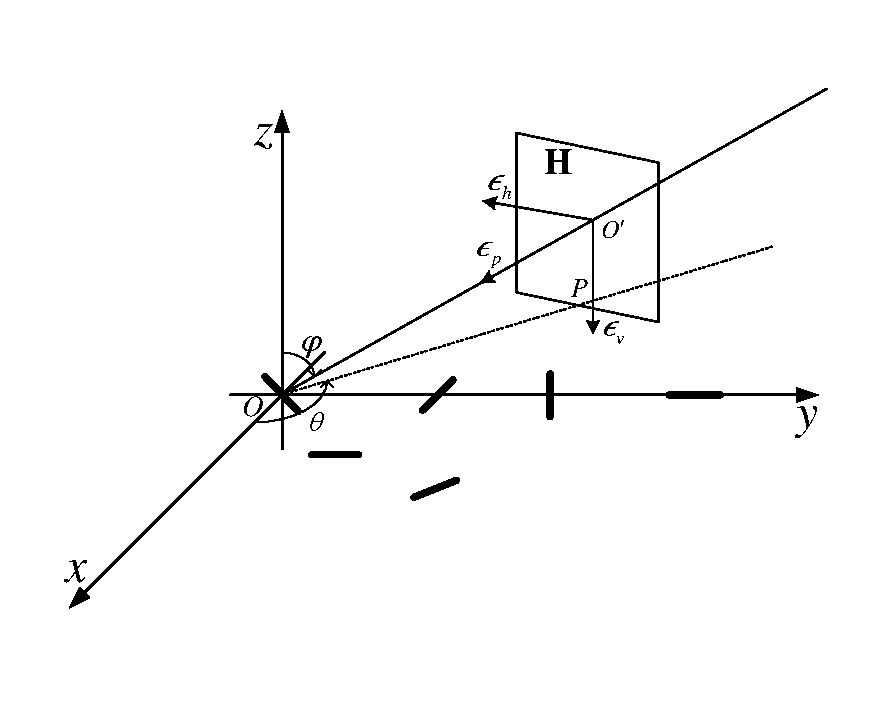
\includegraphics[scale=0.8]{pic/polarized_array.pdf}
    \caption{任意朝向极子组成的极化阵列接收信号模型}
    \label{polarized_array}
\end{figure}
在图\ref{polarized_array}中,向量$\bm{\epsilon}_p(\theta,\phi)$表示入射信号的方向余弦,
其定义由式\eqref{polar_dir_cosine}给出。
\begin{equation}\label{polar_dir_cosine}
    \begin{aligned}
        \bm{\epsilon}_p(\theta,\phi) = 
        -\left[\sin\phi\cos\theta,\sin\phi\sin\theta,\cos\phi\right]^T
    \end{aligned}
\end{equation}
我们假设向量$\bm{\epsilon}_p$是平面$\bm{H}$的法向量,由坡印廷定理可知,入射信号的电场分量$\bm{e}$
总是在平面$\bm{H}$内振动,因此,我们可以利用平面$\bm{H}$内的两线性无关向量为基向量来表出电场分量$\bm{e}$。
\begin{equation}\label{polar_elect_comp}
    \begin{aligned}
        \bm{e}(t) = \zeta_h(t)\bm{\epsilon}_h + \zeta_v(t)\bm{\epsilon}_v
    \end{aligned}
\end{equation}
式\eqref{polar_elect_comp}中,$\bm{\epsilon}_h$和$\bm{\epsilon}_v$都是单位向量,且它们线性无关。
这里需要指出,这个基向量的选取不是唯一的,只要满足\eqref{polar_elect_comp}式即可。
通常情况下,我们选择式\eqref{polar_elect_base_vec}作为电场分量的基向量。
\begin{subequations}\label{polar_elect_base_vec}
    \begin{align}
        \bm{\epsilon}_{h} &=[-\sin \theta, \cos \theta, 0]^{T} \\
        \bm{\epsilon}_{v} &=[\cos \phi \cos \theta, \cos \phi \sin \theta,-\sin \phi]^{T}
    \end{align}
\end{subequations}
式\eqref{polar_elect_base_vec}中,我们将向量$\bm{\epsilon}_h$称作水平向量,他与$xOy$平面平行,
且正交于平面$OO\prime P$。同理,垂直向量$\bm{\epsilon}_v$于水平向量$\bm{\epsilon}_h$正交,
并且与平面$OO^\prime P$和$\bm{H}$的交线平行。实际上向量$\bm{\epsilon}_p$,$\bm{\epsilon}_h$和
$\bm{\epsilon}_v$两两正交,且构成一个直角坐标系。

对于完全极化信号,由Jones向量可知,式\eqref{polar_elect_comp}中的电场极化分量可以被表示为
\begin{equation}\label{polar_elect_zeta_frac}
    \begin{aligned}
        \left[\zeta_{h}(t), \zeta_{v}(t)\right]^{T}=\zeta(t)\left[\cos \gamma, e^{j \eta} \sin \gamma\right]^{T}
    \end{aligned}
\end{equation}
式\eqref{polar_elect_zeta_frac}中,我们称$0\le\gamma\le\pi/2$为极化辅助角,$-\pi\le\eta<\pi$为极化相位差。
结合式\eqref{polar_elect_comp}与\eqref{polar_elect_zeta_frac}我们可以得知,在直角坐标系下,电场分量可以被改写为
\begin{equation}\label{polar_elect_vec_rep}
    \begin{aligned}
        \boldsymbol{e}(t)=\zeta(t)\left[\boldsymbol{\epsilon}_{h}, \boldsymbol{\epsilon}_{v}\right]
        \left[\begin{array}{c}
            \cos \gamma \\
            e^{j \eta} \sin \gamma
            \end{array}
        \right]
    \end{aligned}
\end{equation}
我们将式\eqref{polar_elect_vec_rep}中与极化信息有关的的极化向量表示为$\bm{h}(\gamma,\eta)$,其定义为
\begin{equation}\label{polar_vec}
    \begin{aligned}
        \bm{h}(\gamma, \eta)=\left[\cos \gamma, e^{j \eta} \sin \gamma\right]^{T}
    \end{aligned}
\end{equation}

接下来,我们讨论单个电偶极子的响应。一般情况下,我们都使用短偶极子作为模型,即偶极子长度不超过入射信号波长$10\%$的偶极子。
我们假设有一个短偶极子$l$位于直角坐标系原点,它的极子朝向用角度$\alpha$和$\beta$来描述,如图\ref{dipole_model}所示。
\begin{figure}[h]
    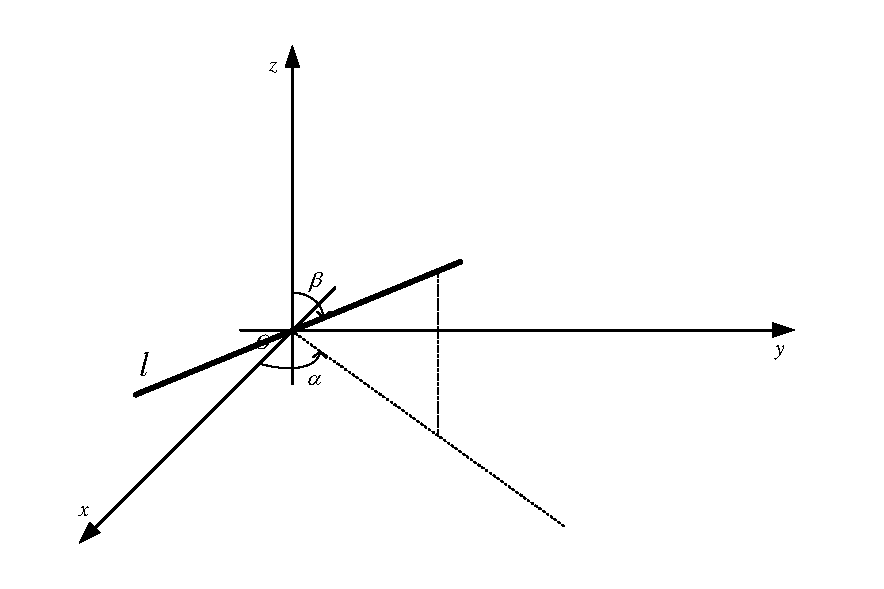
\includegraphics[scale=0.8]{pic/dipole.pdf}
    \caption{任意朝向极子接收信号模型}
    \label{dipole_model}
\end{figure}
我们将极子增益记为向量$\bm{g}$,利用图\ref{dipole_model}中的几何关系,我们可以得到$\bm{g}$的表达式为
\begin{equation}\label{dipole_gain}
    \begin{aligned}
        \bm{g}=\kappa \cdot[\sin \beta \cos \alpha, \sin \beta \sin \alpha, \cos \beta]^{T}
    \end{aligned}
\end{equation}
式\eqref{dipole_gain}中,$\kappa$表示极子与入射信号完全匹配时的增益。

现在,我们来推导由不同朝向极子组成的极化阵列的导向向量。在这个模型中,阵列的响应由两部分组成:
第一部分是阵元位置相对于参考点而引起的相移;第二部分是由入射信号的极化模式引起的相移,
它由极子的朝向,信号的入射方向以及信号的极化参数共同决定。为了不失一般性,
我们可以假设一个完全极化的电磁横波,极化参数为$(\gamma,\eta)$,以$(\theta,\phi)$
入射到一个由$M$个短偶极子组成的共形阵上,其中,阵列的第$m$个极子的坐标由位置向量$\bm{r}_m$决定,第$m$个极子
的朝向由$(\alpha_m,\beta_m)$决定。此时,第$m$个极子的响应为$a_m(\theta,\phi,\gamma,\eta)$,
它由式\eqref{polar_dipole_response}给出。
\begin{equation}\label{polar_dipole_response}
    \begin{aligned}
        a_{m}(\theta, \varphi, \gamma, \eta)=
        u_{m} \bm{g}_{m}^{T}\left[\bm{\epsilon}_{h}, \bm{\epsilon}_{v}\right] \bm{h}
    \end{aligned}
\end{equation}
注意,上式中我们省略了电场极化的强度量$\zeta(t)$和极子完全匹配时的增益$\kappa$,这是因为我们假设入射信号为远场信号,
而远场信号对于短时延$\tau$满足$\zeta(t-\tau)\approx\zeta(t)$。
且组成阵列的每个极子都是完全相同的,即每个极子的$\kappa$都相同,这样对于同一个入射信号,每个极子接收到的$\zeta(t)$
和$\kappa$都是一致的,所以我们省略这两个和强度有关的量并不影响最终的结果。
式\eqref{polar_dipole_response}中,$u_m$表示第$m$个极子的空域相移,由式\eqref{polar_spatial_pd}给出。
\begin{equation}\label{polar_spatial_pd}
    \begin{aligned}
        u_{m}=\exp \left(-j \frac{2 \pi}{\lambda} \bm{r}_{m}^{T} \bm{\epsilon}_{p}\right)
    \end{aligned}
\end{equation}
接着,将式\eqref{polar_dipole_response}改写为向量形式,得到极化阵列的导向向量
\begin{equation}\label{polar_sv}
    \begin{aligned}
        \bm{a}(\theta, \varphi, \gamma, \eta)=
        \operatorname{diag}\left\{\bm{a}_{\bm{s}}(\theta, \varphi)\right\} 
        \bm{G}\left[\bm{\epsilon}_{h}, \bm{\epsilon}_{v}\right] \bm{h}
    \end{aligned}
\end{equation}
我们将式\eqref{polar_sv}中的向量$\bm{a}_s(\theta,\phi)$称为空域导向向量,它的定义由式\eqref{polar_spatial_sv}给出。
\begin{equation}\label{polar_spatial_sv}
    \begin{aligned}
        \bm{a}_{s}(\theta, \varphi)=\left[u_{1}, u_{2}, \cdots, u_{M}\right]^{T}
    \end{aligned}
\end{equation}
而矩阵$\bm{G}$由$M$个向量构成,如式\eqref{dipole_mat}。
\begin{equation}\label{dipole_mat}
    \begin{aligned}
        \bm{G}=\left[\bm{g}_{1}, \bm{g}_{2}, \cdots, \bm{g}_{M}\right]^{T}
    \end{aligned}
\end{equation}
最终,对于一个复振幅为$s(t)$的入射信号,阵列接收的数据$\bm{y}$可以由式\eqref{polar_data}表出。
\begin{equation}\label{polar_data}
    \begin{aligned}
        \bm{y}=s(t) \bm{a}(\theta, \phi, \gamma, \eta)+\bm{n}
    \end{aligned}
\end{equation}
上式中,向量$\bm{n}$表示噪声(或干扰叠加噪声)向量。

\subsection{正交极子的阵列接收信号模型}
本节中,我们介绍阵元极子排布方式相同的阵列模型,其中构成阵列的阵元极子两两正交,
且都与直角坐标系的轴向方向平行。为不失一般性,我们假设一个阵元由三正交电偶极子及三正交磁环构成,如图\ref{ortho_dipole_model}所示。
\begin{figure}[h]
    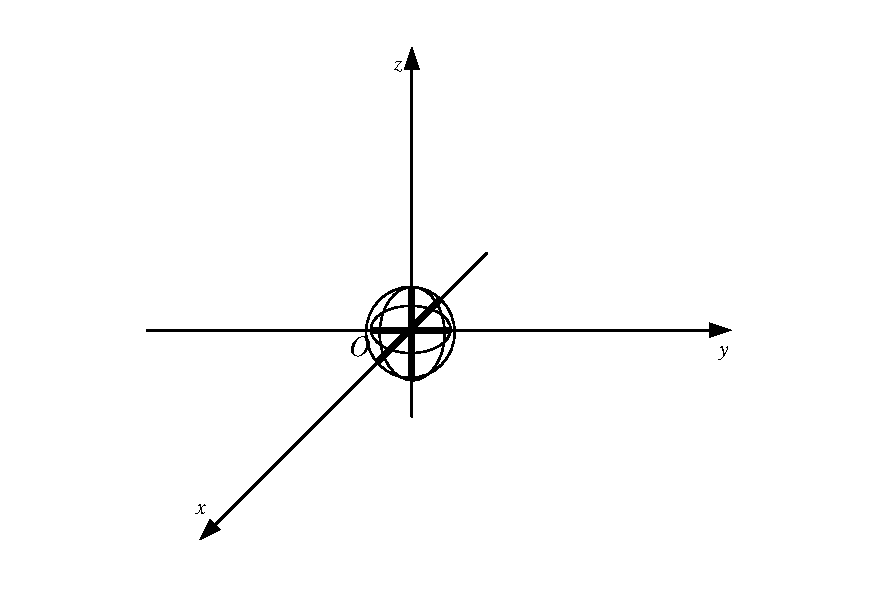
\includegraphics[scale=0.8]{pic/ortho-dipole.pdf}
    \caption{正交极子接收信号模型}
    \label{ortho_dipole_model}
\end{figure}
在上一子节中,我们分析了极化电磁波入射任意电偶极子的模型,在本节中我们加上入射信号的磁场极化分量。
由坡印廷定理可以得知,磁场分量与电场分量位于同一平面,即图\ref{polarized_array}的平面$\bm{H}$内,且与电场分量正交。
因此,我们利用该条件结合式\eqref{polar_elect_base_vec}中电场分量的单位正交基,可以得到磁场分量的两个单位正交基
$\tilde{\bm{\epsilon}}_h$和$\tilde{\bm{\epsilon}}_v$,它们由式\eqref{polar_mag_base_vec}给出。
\begin{subequations}\label{polar_mag_base_vec}
    \begin{align}
        \tilde{\bm{\epsilon}}_h &= 
        \left[\cos\phi\cos\theta,\cos\phi\sin\theta,-\sin\phi\right]^T \\
        \tilde{\bm{\epsilon}}_v &= 
        \left[\sin\theta,-\cos\theta,0\right]^T
    \end{align}
\end{subequations}

我们假设一个由$M$个阵元组成的极化相控阵,其中每个阵元都是由图\ref{ortho_dipole_model}所示的三正交极子和三正交磁环构成的,
由于此时三个两两正交的电偶极子分别沿着三个轴线方向,因此我们可以利用式\eqref{dipole_gain}得到他们的增益矩阵
\begin{subequations}
    \begin{align}
        \bm{G}_x = 
        \begin{bmatrix}
            1 & 0 & 0 \\
            \vdots & \vdots & \vdots \\
            1 & 0 & 0
        \end{bmatrix},
        \bm{G}_y = 
        \begin{bmatrix}
            0 & 1 & 0 \\
            \vdots & \vdots & \vdots \\
            0 & 1 & 0
        \end{bmatrix},
        \bm{G}_z = 
        \begin{bmatrix}
            0 & 0 & 1 \\
            \vdots & \vdots & \vdots \\
            0 & 0 & 1
        \end{bmatrix} \\
        \tilde{\bm{G}}_x = 
        \begin{bmatrix}
            1 & 0 & 0 \\
            \vdots & \vdots & \vdots \\
            1 & 0 & 0
        \end{bmatrix},
        \tilde{\bm{G}}_y = 
        \begin{bmatrix}
            0 & 1 & 0 \\
            \vdots & \vdots & \vdots \\
            0 & 1 & 0
        \end{bmatrix},
        \tilde{\bm{G}}_z = 
        \begin{bmatrix}
            0 & 0 & 1 \\
            \vdots & \vdots & \vdots \\
            0 & 0 & 1
        \end{bmatrix}
    \end{align}
\end{subequations}
上式中,矩阵$\bm{G}_{(\cdot)}\in\mathbb{R}^{M\times3}$表示相应轴线方向上电偶极子的增益矩阵,
$\tilde{\bm{G}}_{(\cdot)}\in\mathbb{R}^{M\times3}$表示相应轴线方向上磁环的增益矩阵。

我们利用上一节中的结论,可以得到期望信号的电-磁极化分量$\bm{p}(\theta,\phi,\gamma,\eta)\in\mathbb{C}^{6\times1}$,
如式\eqref{ortho_dipole_respon}所示。
\begin{equation}\label{ortho_dipole_respon}
    \begin{aligned}
        \bm{p}(\theta,\phi,\gamma,\eta) = 
        \begin{bmatrix}
            \bm{\epsilon}_h & \bm{\epsilon}_v \\
            \tilde{\bm{\epsilon}}_h & \tilde{\bm{\epsilon}}_v
        \end{bmatrix}
        \begin{bmatrix}
            \cos\gamma \\ e^{j\eta}\sin\gamma
        \end{bmatrix}
    \end{aligned}
\end{equation}
然后结合上一节中的\eqref{polar_sv}式,我们可以得到阵列的导向向量$\bm{a}(\theta,\phi,\gamma,\eta)\in\mathbb{C}^{6M\times1}$
\begin{equation}\label{polar_ortho_sv_comp}
    \begin{aligned}
        \bm{a}(\theta,\phi,\gamma,\eta) = 
        \begin{bmatrix}
            \operatorname{diag}\left\{\bm{a}_s(\theta,\phi)\right\} \\
            \vdots \\
            \operatorname{diag}\left\{\bm{a}_s(\theta,\phi)\right\}
        \end{bmatrix}
        \begin{bmatrix}
            \bm{G}_x & \tilde{\bm{G}}_x \\
            \bm{G}_y & \tilde{\bm{G}}_y \\
            \bm{G}_z & \tilde{\bm{G}}_z
        \end{bmatrix}
        \begin{bmatrix}
            \bm{\epsilon}_h & \bm{\epsilon}_v \\
            \tilde{\bm{\epsilon}}_h & \tilde{\bm{\epsilon}}_v
        \end{bmatrix}
        \begin{bmatrix}
            \cos\gamma \\ e^{j\eta}\sin\gamma
        \end{bmatrix}
    \end{aligned}
\end{equation}
上式中,向量$\bm{a}_s(\theta,\phi)\in\mathbb{C}^{M\times1}$同上一节一样表示空域导向向量。
由于极子和磁环的增益矩阵$\bm{G}_{(\cdot)}$和$\tilde{\bm{G}}_{(\cdot)}$均为某一列全是1的矩阵,
因此可以借助Kronecker积的性质,将式\eqref{polar_ortho_sv_comp}改写为式\eqref{polar_ortho_sv}。
\begin{equation}\label{polar_ortho_sv}
    \begin{aligned}
        \bm{a}(\theta,\phi,\gamma,\eta) = 
        \bm{a}_s(\theta,\phi) \otimes 
        \left(
            \begin{bmatrix}
                \bm{\epsilon}_h & \bm{\epsilon}_v \\
                \tilde{\bm{\epsilon}}_h & \tilde{\bm{\epsilon}}_v
            \end{bmatrix}
            \begin{bmatrix}
                \cos\gamma \\ e^{j\eta}\sin\gamma
            \end{bmatrix}
        \right)
    \end{aligned}
\end{equation}
上式中,$\otimes$表示Kronecker积。式\eqref{polar_ortho_sv}即为正交极子极化阵导向向量的一般表达式。

\section{双正交极子的极化相控阵单脉冲测向}
本节中,我们探讨双正交极子组成的极化阵列单脉冲测向问题。双正交极子即阵元由两个正交的电偶极子(或磁环)构成,
我们以双正交电偶极子组成的均匀线阵为例,给出一种双通道数据融合的测向方法,并给出该方法的误差分析和仿真结果。

\subsection{双通道数据融合方法}
考虑一个双正交电偶极子组成的均匀线阵,阵元间距为半波长,共有$M$个阵元,$2M$个电偶极子,如图\ref{dual_ortho_ULA_fig}所示。
\begin{figure}[h]
    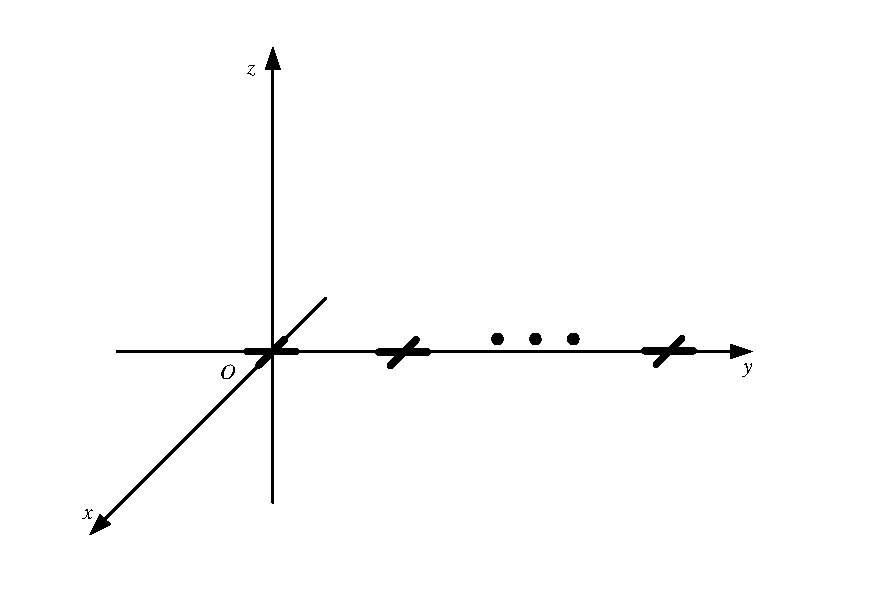
\includegraphics[scale=0.8]{pic/dual_ortho_ULA.pdf}
    \caption{双正交极子组成的均匀线阵}
    \label{dual_ortho_ULA_fig}
\end{figure}
图\ref{dual_ortho_ULA_fig}中,构成阵元的两正交偶极子分别沿$x$轴方向和$y$轴方向排列。
我们借助上一节中的\eqref{polar_ortho_sv}式,可以得到该阵列的导向向量$\bm{a}(\phi,\gamma,\eta)\in\mathbb{C}^{2M\times1}$,
注意,这里我们取方位角$\theta=90^\circ$,即信号在$yOz$平面内,且规定俯仰角的定义域为$\phi\in\left[-90^\circ,90^\circ\right]$。
\begin{equation}\label{dual_ortho_ULA_sv}
    \begin{aligned}
        \bm{a}(\phi,\gamma,\eta) &= 
        \bm{a}_s(\phi) \otimes 
        \left(
            \begin{bmatrix}
                -1 & 0 \\
                0 & \cos\phi
            \end{bmatrix}
            \begin{bmatrix}
                \cos\gamma \\ e^{j\eta}\sin\gamma
            \end{bmatrix}
        \right) \\
        &=
        \bm{a}_s(\phi) \otimes 
        \begin{bmatrix}
            -\cos\gamma \\ e^{j\eta}\sin\gamma\cos\phi    
        \end{bmatrix}
    \end{aligned}
\end{equation}
上式中的空域导向向量$\bm{a}_s(\phi)$可以由第二章中的式\eqref{sv_ULA}得到。
因此,对于一个复振幅为$s(t)$,入射方向为$\phi$且极化参数为$(\gamma,\eta)$的入射信号,阵列接收到的数据向量
$\bm{y}\in\mathbb{C}^{2M\times1}$为
\begin{equation}
    \begin{aligned}
        \bm{y} = s(t)\bm{a}(\phi,\gamma,\eta) + \bm{n}
    \end{aligned}
\end{equation}
上式中,向量$\bm{n}\in\mathbb{C}^{2M\times1}$为噪声向量,在这里,我们规定$\bm{y}$的第$1$至第$M$行为阵列的水平通道,
记为向量$\bm{y}_h$,而第$M+1$行至$2M$行为阵列的垂直通道,记为$\bm{y}_v$。由于式\eqref{dual_ortho_ULA_sv}中导向向量
Kronecker积的特性,我们实际上可以将信号的极化分量归并称为信号的一部分,并且将信号模型重写为
\begin{subequations}
    \begin{align}
        \bm{y}_h = A_h\bm{a}_s(\phi) + \bm{n}_h \\
        \bm{y}_h = A_h\cos\phi\bm{a}_s(\phi) + \bm{n}_h
    \end{align}
\end{subequations}
上式中,期望信号的水平复振幅$A_h=-\cos\gamma s(t)$,垂直复振幅$A_v=\exp(j\eta)\sin\gamma s(t)$。

接下来,我们以均匀线阵的半阵法为例,解析双通道信息融合的一般过程。
首先利用第二章中的半阵法得到和差波束权$\bm{w}_\Sigma$和$\bm{w}_\Delta$,对于两个通道的极子,它们的空间相对位置是一致的,
因此可以共享同一组和差波束权。然后利用半阵法的单脉冲比函数$f(\phi)$与水平和垂直通道的接收数据,分别得到两个通道的角度估计值,
即
\begin{subequations}\label{dual_phi_hat}
    \begin{align}
        \hat{\phi}_h &= f^{-1}\left(\frac{\bm{w}_\Delta^H\bm{y}_h}{\bm{w}_\Sigma^H\bm{y}_h}\right) \\
        \hat{\phi}_v &= f^{-1}\left(\frac{\bm{w}_\Delta^H\bm{y}_v}{\bm{w}_\Sigma^H\bm{y}_v}\right)
    \end{align}
\end{subequations}
式\eqref{dual_phi_hat}中,$f^{-1}(\cdot)$表示单脉冲比的反函数。注意,垂直通道的导向向量前多一个$\cos\phi$的系数,
但进过差和比$\Delta/\Sigma$后抵消了,因此不影响测向过程。

然后我们假设噪声向量$\bm{n}\sim\mathcal{CN}(0,\sigma_n^2\bm{I})$,即满足独立同分布的零均值复高斯分布。
这样就可以利用最大似然方法得到两个通道信号复振幅的估计值\cite{Ma}。
\begin{subequations}\label{dual_amp_hat}
    \begin{align}
        \hat{A}_h &= \frac{\bm{a}_s^H(\hat{\phi}_h)\bm{y}_h}{M} \\
        \hat{A}_v &= \frac{\cos\hat{\phi}\bm{a}_s^H(\hat{\phi}_v)\bm{y}_v}{M}
    \end{align}
\end{subequations}
最后,我们以水平通道和垂直通道的信号功率作为权值,将两通道的估计值做加权平均融合,得到最终的估计值$\hat{\phi}$,
如式\eqref{merge_hat}所示。
\begin{equation}\label{merge_hat}
    \begin{aligned}
        \hat{\phi} = 
        \frac{\hat{\phi}_h\left|\hat{A}_h\right|^2+\hat{\phi}_v\left|\hat{A}_v\right|^2}
        {\left|\hat{A}_h\right|^2+\left|\hat{A}_v\right|^2}
    \end{aligned}
\end{equation}
在未知期望信号极化参数的条件下,该方法使用两通道分别求解,并以功率作为权值进行信息融合,保证最终给出一个可接受的结果。

\subsection{性能分析}

\subsection{仿真}

\section{极子摆放方式不同时的极化相控阵单脉冲测向}
当组成阵列的极子朝向各不相同时,导向向量中的空域时延$\bm{a}_s(\theta,\phi)$无法和极化导致的幅相变化分离,
因此传统的测向方法无法直接应用到该模型下,所以本节中我们从信号模型的统计信息入手,借助似然函数完成单脉冲测向过程,
并在得到入射信号的角度信息后给出一种极化参数的估计方法。

\subsection{基本原理}
我们假设一个由$M$个极子组成的极化阵列,$M$个极子的摆放方式由矩阵$\bm{G}$决定,
一个极化参数为$(\gamma,\eta)$的远场窄带信号以角度$(\theta,\phi)$入射到该阵列上。

首先可以假设干扰叠加噪声向量$\bm{n}$服从一个均值为零,协方差矩阵为$\bm{Q}\in\mathbb{C}^{M\times M}$的复高斯分布,
即$\bm{n}\sim\mathcal{CN}(0,\bm{Q})$。在该假设下,接收信号$\bm{y}$的概率密度函数可以写为
\begin{equation}\label{polar_pdf}
    \begin{aligned}
        p(\bm{y} \mid \bm{\theta}, \gamma, \eta, s(t))= 
        \frac{1}{\pi^{M} \operatorname{det}(\bm{Q})} \exp 
        \left\{
            -[\bm{y}-s(t) \bm{a}(\bm{\theta})]^{H} 
            \bm{Q}^{-1}[\bm{y}-s(t) \bm{a}(\bm{\theta})]
            \right\}
    \end{aligned}
\end{equation}
然后对式\eqref{polar_pdf}中的概率密度函数取自然对数并舍弃掉所有常量得到
\begin{equation}\label{log_lf}
    \begin{aligned}
        \mathcal{L}(\bm{\theta}, \gamma, \eta, s(t)) &=
        \ln p(\bm{y} \mid \bm{\theta}, \gamma, \eta, s(t)) \\
        &=-[\bm{y}-s(t) \bm{a}(\bm{\theta},\gamma,\eta)]^{H} \bm{Q}^{-1}[\bm{y}-s(t) \bm{a}(\bm{\theta,\gamma,\eta})]
    \end{aligned}
\end{equation}
式\eqref{log_lf}中,向量$\bm{\theta}=\left[\theta,\phi\right]^T$表示期望信号的入射角度。
我们感兴趣的部分是期望信号的入射角度$\bm{\theta}$,所以我们需要导出一个仅关于参数$\bm{\theta}$的对数似然函数。
因此我们定义矩阵$\bm{A}\in\mathbb{C}^{M\times2}$和向量$\bm{s}\in\mathbb{C}^{2\times1}$。
\begin{subequations}\label{polar_A_nd_s}
    \begin{align}
            \bm{A}(\theta, \varphi) &=
            \operatorname{diag}\left\{\bm{a}_{s}(\theta, \varphi)\right\} \bm{G}
            \left[\bm{\epsilon}_{h}, \bm{\epsilon}_{v}\right] \\
            \bm{s}(\gamma, \eta) &=s(t) \bm{h}=\left[s(t) \cos \gamma, s(t) e^{j \eta} \sin \gamma\right]^{T}
    \end{align}
\end{subequations}
然后将式\eqref{polar_A_nd_s}代入\eqref{log_lf}得到
\begin{equation}\label{polar_log_lf_As}
    \begin{aligned}
        \mathcal{L}(\bm{\theta}, \bm{s})=
        -[\bm{y}-\bm{A} \bm{s}]^{H}{\bm{Q}}^{-1}[\bm{y}-\bm{A} \bm{s}]
    \end{aligned}
\end{equation}
与最大似然方法类似,我们对向量$\bm{s}$求最小二乘解得到其估计量$\hat{\bm{s}}$。
\begin{equation}\label{polar_s_hat}
    \begin{aligned}
        \hat{\bm{s}}=
        \left[\bm{A}^{H}(\bm{\theta}) \bm{Q}^{-1} \bm{A}(\bm{\theta})\right]^{-1} 
        \bm{A}^{H}(\bm{\theta}) \bm{Q}^{-1} \bm{y}
    \end{aligned}
\end{equation}
接着将式\eqref{polar_s_hat}代入\eqref{polar_log_lf_As},并去掉常数项,
得到关于期望信号入射角度$\bm{\theta}$的对数似然函数$\mathcal{L}(\bm{\theta})$。
\begin{equation}\label{polar_lf}
    \begin{aligned}
        \mathcal{L}(\bm{\theta})=
        \bm{y}^{H} \bm{Q}^{-1} \bm{A}
        \left(\bm{A}^{H} \bm{Q}^{-1} \bm{A}\right)^{-1} \bm{A}^{H} \bm{Q}^{-1} \bm{y}
    \end{aligned}
\end{equation}
现在,我们就可以将角度估计问题转化为一个优化问题,即式\eqref{polar_lf_opt}。
\begin{equation}\label{polar_lf_opt}
    \begin{aligned}
        &\max_{\bm{\theta}} ~ \mathcal{L}(\bm{\theta}) \\
        &\text{s.t.} ~ -\pi\leqslant\theta, 0\leqslant\phi\leqslant\pi
    \end{aligned}
\end{equation}

我们注意到,式\eqref{polar_lf}中的矩阵$\left(\bm{A}^H\bm{Q}^{-1}\bm{A}\right)^{-1}$是一个Hermite矩阵,
因此我们易知它的矩阵平方根一定存在。利用该性质,我们可以将式\eqref{polar_lf}重写为
\begin{equation}\label{polar_lf_W}
    \begin{aligned}
        \mathcal{L}(\bm{\theta}) = \bm{y}^H\bm{W}(\bm{\theta})\bm{W}^H(\bm{\theta})\bm{y}
    \end{aligned}
\end{equation}
上式中,矩阵$\bm{W}(\bm{\theta})\in\mathbb{M\times2}$定义为
\begin{equation}\label{polar_W_mat}
    \begin{aligned}
        \bm{W}(\bm{\theta}) = \bm{Q}^{-1}\bm{A}(\bm{\theta})
        \left(\bm{A}^H(\bm{\theta})\bm{Q}^{-1}\bm{A}(\bm{\theta})\right)^{-1/2}
    \end{aligned}
\end{equation}
注意在式\eqref{polar_W_mat}中上标$\cdot^{1/2}$表示矩阵平方根。我们易知$\mathcal{L}(\bm{\theta})$是一个凹函数,
即它在定义域上有全局最大值,并且它是严格大于0的。

为便于后续的公式推导,我们对\eqref{polar_lf_W}式中的$\mathcal{L}(\bm{\theta})$取自然对数得
$F(\bm{\theta})=\ln\mathcal{L}(\bm{\theta})$,这样并不改变它的单调性和凹凸性。
与第四章中的最大似然方法类似,我们给出牛顿公式,即式\eqref{polar_newton_itr}。
\begin{equation}\label{polar_newton_itr}
    \hat{\bm{\theta}} = \bm{\theta}_0 - \bm{H}^{-1}\nabla F(\bm{\theta})
\end{equation}
上式中,向量$\bm{\theta}_0$表示待估计角度$\bm{\theta}$的初值,矩阵$\bm{H}$表示函数$F(\bm{\theta})$的海森矩阵,
$\nabla F(\bm{\theta})$表示函数$F(\bm{\theta})$的梯度,即雅可比矩阵。它们的定义由式\eqref{polar_Hessian_Jacb}给出。
\begin{subequations}\label{polar_Hessian_Jacb}
    \begin{align}
        \bm{H} &=
        \begin{bmatrix}
            F_{\theta\theta} & F_{\theta\phi} \\
            F_{\theta\phi}   & F_{\phi\phi}
        \end{bmatrix} \\
        \nabla F(\bm{\theta}) &= \left[F_\theta,F_\phi\right]^T
    \end{align}
\end{subequations}
式中,$F_\theta$表示一阶偏导数$\partial F/\partial\theta$,而$F_{\theta\phi}$表示二阶偏导数$\partial^2 F/\partial\theta\phi$,
其余同理。
牛顿法要求一个初值才能进行估计,幸运的是,在单脉冲测向系统中,我们恰好有一个波束指向角$\bm{\theta}_0$。
期望信号的真实方向$\bm{\theta}_s$往往与波束指向角接近(一般在3dB主瓣宽度内),所以我们可以用单步迭代的方式代替多步迭代
以减小计算量。剩下的部分我们将着重于$\bm{F}(\bm{\theta})$一二阶偏导数的导出。

利用式\eqref{polar_lf_W}可以得到一阶偏导数$F_\theta$。
\begin{equation}\label{polar_F_theta}
    \begin{aligned}
        F_\theta &= 
        \frac{\bm{y}^H\bm{W}_\theta\bm{W}^H\bm{y} + \bm{y}^H\bm{W}\bm{W}^H_\bm{\theta}\bm{y}}
        {\bm{y}^H\bm{W}\bm{W}^H\bm{y}} \\
        &= 2\frac{\operatorname{Re}\left\{\bm{y}^H\bm{W}_\theta\bm{W}^H\bm{y}\right\}}
        {\bm{y}^H\bm{W}\bm{W}^H\bm{y}}
    \end{aligned}
\end{equation}
式\eqref{polar_F_theta}中,矩阵$\bm{W}_\theta$的定义如下。
\begin{equation}\label{polar_W_theta}
    \begin{aligned}
        \bm{W}_\theta = 
        \bm{Q}^{-1}\bm{A}_\theta\left(\bm{A}^H\bm{Q}^{-1}\bm{A}\right)^{-1/2} - 
        \bm{W}\left(\bm{A}^H\bm{Q}^{-1}\bm{A}\right)^{-1}
        \operatorname{Re}\left\{\bm{A}^H_\theta\bm{Q}^{-1}\bm{A}\right\}
    \end{aligned}
\end{equation}
为了简化符号,我们给出定义式\eqref{polar_D_mu_def}。
\begin{subequations}\label{polar_D_mu_def}
    \begin{align}
        \bm{D}^{\theta} &= \bm{Q}^{-1}\bm{A}_\theta\left(\bm{A}^H\bm{Q}^{-1}\bm{A}\right)^{-1/2} \\
        \bm{\mu}^\theta &= \left(\bm{A}^H\bm{Q}^{-1}\bm{A}\right)^{-1}
        \operatorname{Re}\left\{\bm{A}^H_\theta\bm{Q}^{-1}\bm{A}\right\}
    \end{align}
\end{subequations}
然后将式\eqref{polar_D_mu_def}代入\eqref{polar_W_theta}得到
\begin{equation}
    \begin{aligned}
        \bm{W}_\theta = \bm{D}^\theta - \bm{W}\bm{\mu}^\theta
    \end{aligned}
\end{equation}
在式\eqref{polar_W_theta}和\eqref{polar_D_mu_def}中,导数$\bm{A}_\theta$的定义由式\eqref{polar_A_theta}给出。
\begin{equation}\label{polar_A_theta}
    \begin{aligned}
        \bm{A}_\theta = 
        \operatorname{diag}\left\{\frac{\bm{a}_s(\theta,\phi)}{\partial\theta}\right\}
        \bm{G}\left[\bm{\epsilon}_h,\bm{\epsilon}_v\right] + 
        \operatorname{diag}\left\{\bm{a}_s(\theta,\phi)\right\}\bm{G}
        \left[\frac{\partial\bm{\epsilon}_h}{\partial\theta},\frac{\partial\bm{\epsilon}_v}{\partial\theta}\right]
    \end{aligned}
\end{equation}
上式中,$\partial\bm{a}_s(\theta,\phi)/\partial\theta$和
$\left[\partial\bm{\epsilon}_h/\partial\theta,\partial\bm{\epsilon}_v/\partial\theta\right]$的定义如下。
\begin{subequations}\label{polar_a_s_nd_epsilon_theta}
    \begin{align}
        \left[\frac{\partial\bm{a}_s(\theta,\phi)}{\partial\theta}\right]_m &= 
        -j\frac{2\pi}{\lambda}\bm{r}^T_m\frac{\partial\bm{\epsilon}_p}{\partial\theta}
        \exp\left(-j\frac{2\pi}{\lambda}\bm{r}^T_m\bm{\epsilon}_p\right) \\
        \left[\frac{\partial\bm{\epsilon}_h}{\partial\theta},\frac{\partial\bm{\epsilon}_v}{\partial\theta}\right]
        &=
        \begin{bmatrix}
            -\cos\theta & -\cos\phi\sin\theta \\
            -\sin\theta & \cos\phi\cos\theta \\
            0           & 0
        \end{bmatrix}
    \end{align}
\end{subequations}
式子中的$\left[\cdot\right]_m$表示向量的第$m$个元素。我们可以用相同的方式导出$\bm{W}_\phi$的表达式。

紧接着,我们导出函数$F(\bm{\theta})$的二阶偏导数,$F_{\theta\phi}$的定义由式\eqref{polar_F_theta_phi}给出。
\begin{equation}\label{polar_F_theta_phi}
    \begin{aligned}
        F_{\theta\phi} = 
        2\frac{\operatorname{Re}\left\{\bm{y}^H\bm{W}_{\theta\phi}\bm{W}^H\bm{y}\right\}}
        {\bm{y}^H\bm{W}\bm{W}^H\bm{y}} + 
        2\frac{\operatorname{Re}\left\{\bm{y}^H\bm{W}_{\theta}\bm{W}^H_\phi\bm{y}\right\}}
        {\bm{y}^H\bm{W}\bm{W}^H\bm{y}} - F_\theta F_\phi
    \end{aligned}
\end{equation}
上式中,矩阵$\bm{W}$的二阶导数由下式给出。
\begin{equation}\label{polar_W_theta_phi}
    \begin{aligned}
        \bm{W}_{\theta\phi} = \bm{D}_\phi^\theta - \bm{W}_\phi\bm{\mu}^\theta - \bm{W}\bm{\mu}^\theta_\phi
    \end{aligned}
\end{equation}
式\eqref{polar_W_theta_phi}中,矩阵$\bm{D}^\theta_\phi$和$\mu^\theta_\phi$的定义如式所示。
\begin{subequations}
    \begin{align}
        \bm{D}^\theta_\phi &= \bm{Q}^{-1}\bm{A}_{\theta\phi}
        \left(\bm{A}^H\bm{Q}^{-1}\bm{A}\right)^{-1/2} - \bm{D}^\theta\bm{\mu}^\theta \\
        \bm{\mu}^\theta_\phi &= 
        -2\left(\bm{A}^H\bm{Q}^{-1}\bm{A}\right)^{-1}\bm{\mu}^\phi
        \operatorname{Re}\left\{\bm{A}^H_\theta\bm{Q}^{-1}\bm{A}\right\} \\ &+  
        \left(\bm{A}^H\bm{Q}^{-1}\bm{A}\right)^{-1}
        \operatorname{Re}\left\{\bm{A}^H_{\theta\phi}\bm{Q}^{-1}\bm{A} + \bm{A}^H_\phi\bm{Q}^{-1}\bm{A}_\phi\right\}
    \end{align}
\end{subequations}
接着借助式\eqref{polar_A_theta},我们可以得到矩阵$\bm{A}$的二阶偏导数$\bm{A}_{\theta\phi}$,
它的定义由式\eqref{polar_A_theta_phi}表出。
\begin{equation}\label{polar_A_theta_phi}
    \begin{aligned}
        \bm{A} &= \operatorname{diag}\left\{\frac{\partial^2\bm{a}_s(\theta,\phi)}{\partial\theta\partial\phi}\right\}
        \bm{G}\left[\bm{\epsilon}_h,\bm{\epsilon}_v\right] + 
        \operatorname{diag}\left\{\bm{a}_s(\theta,\phi)\right\}\bm{G}
        \left[
            \frac{\partial^2\bm{\epsilon}_h}{\partial\theta\partial\phi},
            \frac{\partial^2\bm{\epsilon}_v}{\partial\theta\partial\phi}
        \right] \\ &+ 
        \operatorname{diag}\left\{\frac{\partial\bm{a}_s(\theta,\phi)}{\partial\theta}\right\}\bm{G}
        \left[
            \frac{\partial\bm{\epsilon}_h}{\partial\phi},
            \frac{\partial\bm{\epsilon}_v}{\partial\phi}
        \right] + 
        \operatorname{diag}\left\{\frac{\partial\bm{a}_s(\theta,\phi)}{\partial\phi}\right\}\bm{G}
        \left[
            \frac{\partial\bm{\epsilon}_h}{\partial\theta},
            \frac{\partial\bm{\epsilon}_v}{\partial\theta}
        \right]
    \end{aligned}
\end{equation}
上式中的$\partial^2\bm{a}_s/\partial\theta\partial\phi$和
$\partial^2\left[\bm{\epsilon}_h,\bm{\epsilon}_v\right]/\partial\theta\partial\phi$可以由式
\eqref{polar_a_s_nd_epsilon_theta}直接计算得到。由于求导后的表达式较为复杂,因此我们在这里不将其一一给出。
函数$F(\bm{\theta})$的其它两个二阶导数$F_{\theta\theta}$和$F_{\phi\phi}$可以以相同的方式得到。

最后,我们利用函数$F(\bm{\theta})$的一二阶导数构造出式\eqref{polar_Hessian_Jacb}中的海森矩阵和雅可比矩阵,
同时将阵列的波束指向$\bm{\theta}_0$作为初值,并结合式\eqref{polar_newton_itr}得到期望信号入射角度的估计值$\hat{\bm{\theta}}$。

在得到角度估计值$\hat{\bm{\theta}}$后,我们可以进一步得到极化参数$\gamma$和$\eta$的估计值。
首先利用$\bm{s}$的最小二乘解,即\eqref{polar_s_hat}式得到信号向量的估计值$\hat{\bm{s}}$。
利用向量$\bm{s}$的定义式\eqref{polar_A_nd_s}我们显然能够得到式\eqref{polar_args_hat}。
\begin{equation}\label{polar_args_hat}
    \begin{aligned}
        \frac{\left[\hat{\bm{s}}\right]_2}{\left[\hat{\bm{s}}\right]_1} = 
        e^{j\hat{\eta}}\tan\hat{\gamma}
    \end{aligned}
\end{equation}
上式中,$\left[\cdot\right]_m$表示向量的第$m$个元素。由于极化参数的定义域为
$0\le\gamma\le\pi/2$和$-\pi\le\eta<\pi$,所以我们可以用反三角函数表示它们的估计量
\begin{subequations}\label{polar_args_hat_arc}
    \begin{align}
        \hat{\gamma} &= 
        \arctan\left(\left|\frac{\left[\hat{\bm{s}}\right]_2}{\left[\hat{\bm{s}}\right]_1}\right|\right) \\
        \hat{\eta} &= 
        \arg\left(\frac{\left[\hat{\bm{s}}\right]_2}{\left[\hat{\bm{s}}\right]_1}\right)
    \end{align}
\end{subequations}
式\eqref{polar_args_hat_arc}中,$\left|\cdot\right|$表示取幅值,$\arg(\cdot)$表示取幅角。
至此,该模型下的单脉冲测向过程导出完毕。在接下来的子节中,我们给出仿真结果对比。

\subsection{仿真结果}
为了展示本节算法的性能,我们给出一些数值仿真结果。考虑一个由短偶极子对组成的均匀圆阵,
如图\ref{polar_circular_array}所示。
\begin{figure}[h]
    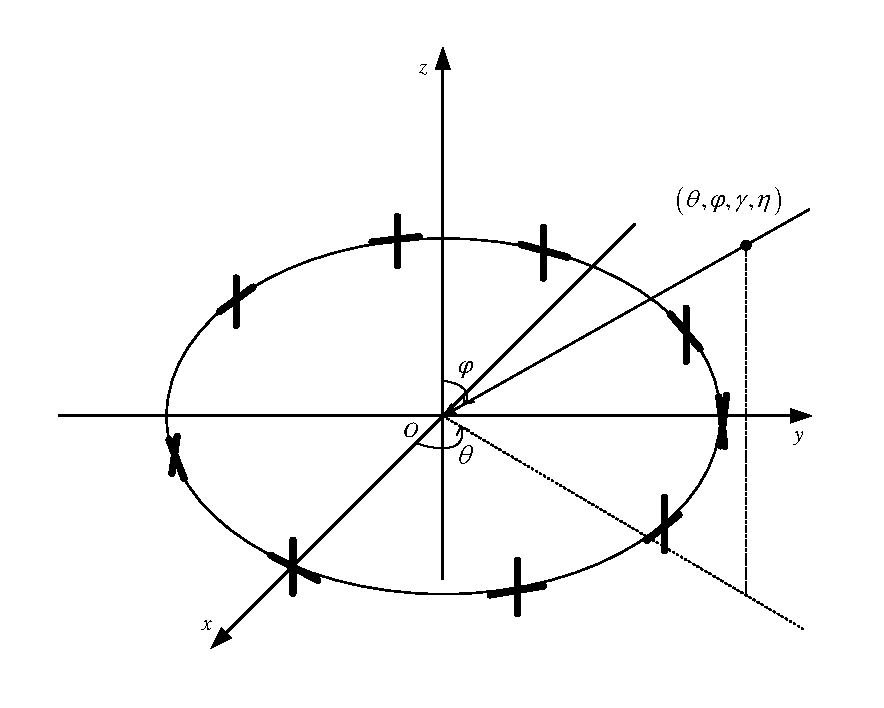
\includegraphics[scale=0.8]{pic/circular_array.pdf}
    \caption{两组短偶极子组成的均匀圆阵}
    \label{polar_circular_array}
\end{figure}
其中,与$z$轴平行的偶极子构成一组,而其余沿圆环切线方向的偶极子构成另一组。
本方法将与最大似然方法\cite{Nickel_93}和比幅法\cite{Mosca}进行比较。
由于这些传统相控阵测向方法不适用于组成阵列的各极子朝向不同的情况,
因此我们将其分为两组分别测向。我们将与$z$轴平行的偶极子定义为垂直通道,极子增益矩阵为$\bm{G}_v$。
沿圆环切向方向的偶极子构成水平通道,增益矩阵为$\bm{G}_h$。最大似然方法只能用于垂直通道,而比幅测向法只能在两个通道上独立进行。
作为对比,我们提出的方法是一种联合测向方法,这意味着我们可以将两个通道的极子并列于同一个表达式。在这种情况下,
导向向量的定义如式\eqref{polar_circular_array_sv}所示。
\begin{equation}\label{polar_circular_array_sv}
    \begin{aligned}
        \bm{a}(\theta,\phi,\gamma,\eta) = 
        \begin{bmatrix}
            \operatorname{diag}\left\{\bm{a}_s(\theta,\phi)\right\}\bm{G}_h \\
            \operatorname{diag}\left\{\bm{a}_s(\theta,\phi)\right\}\bm{G}_v
        \end{bmatrix}
        \left[\bm{\epsilon}_h,\bm{\epsilon}_v\right]\bm{h}
    \end{aligned}
\end{equation}

在所有的仿真中,均匀圆阵都是由$9$对偶极子组成,且半径为$1m$(如图\ref{polar_circular_array})。
期望信号为300MHz的远场窄带信号,入射方位角$\theta_s=42^\circ$,俯仰角为$\phi_s=48^\circ$。
而阵列波束指向$(\theta_0,\phi_0)$为$(45^\circ,45^\circ)$。快拍数$N$为200.信噪比为15dB。
结果中的每次估计量都是由$L=1000$次蒙特卡洛实验得到的。其测角性能由均方根误差(RMSE)衡量,
即式\eqref{RMSE_formula}。
\begin{equation}\label{RMSE_formula}
    \begin{aligned}
        \text{RMSE} = \sqrt{\frac{1}{L}\sum_{l=1}^L\left(\hat{\theta}_l-\theta\right)^2}
    \end{aligned}
\end{equation}
上式中,$(\cdot)_l$表示第$l$次蒙特卡洛实验的估计结果。

仿真A:无干扰时的测向性能对比

在第一个仿真中,取期望信号的极化相位差$\eta_s=0$。极化辅助角$\gamma_s$从$0$变化到$\pi/2$。
各算法测角误差对比如图\ref{Polar_RMSE_jammer_free}所示。
\begin{figure}[h]
    \subfloat[]{
        \label{Polar_RMSE_jammer_free_a}
        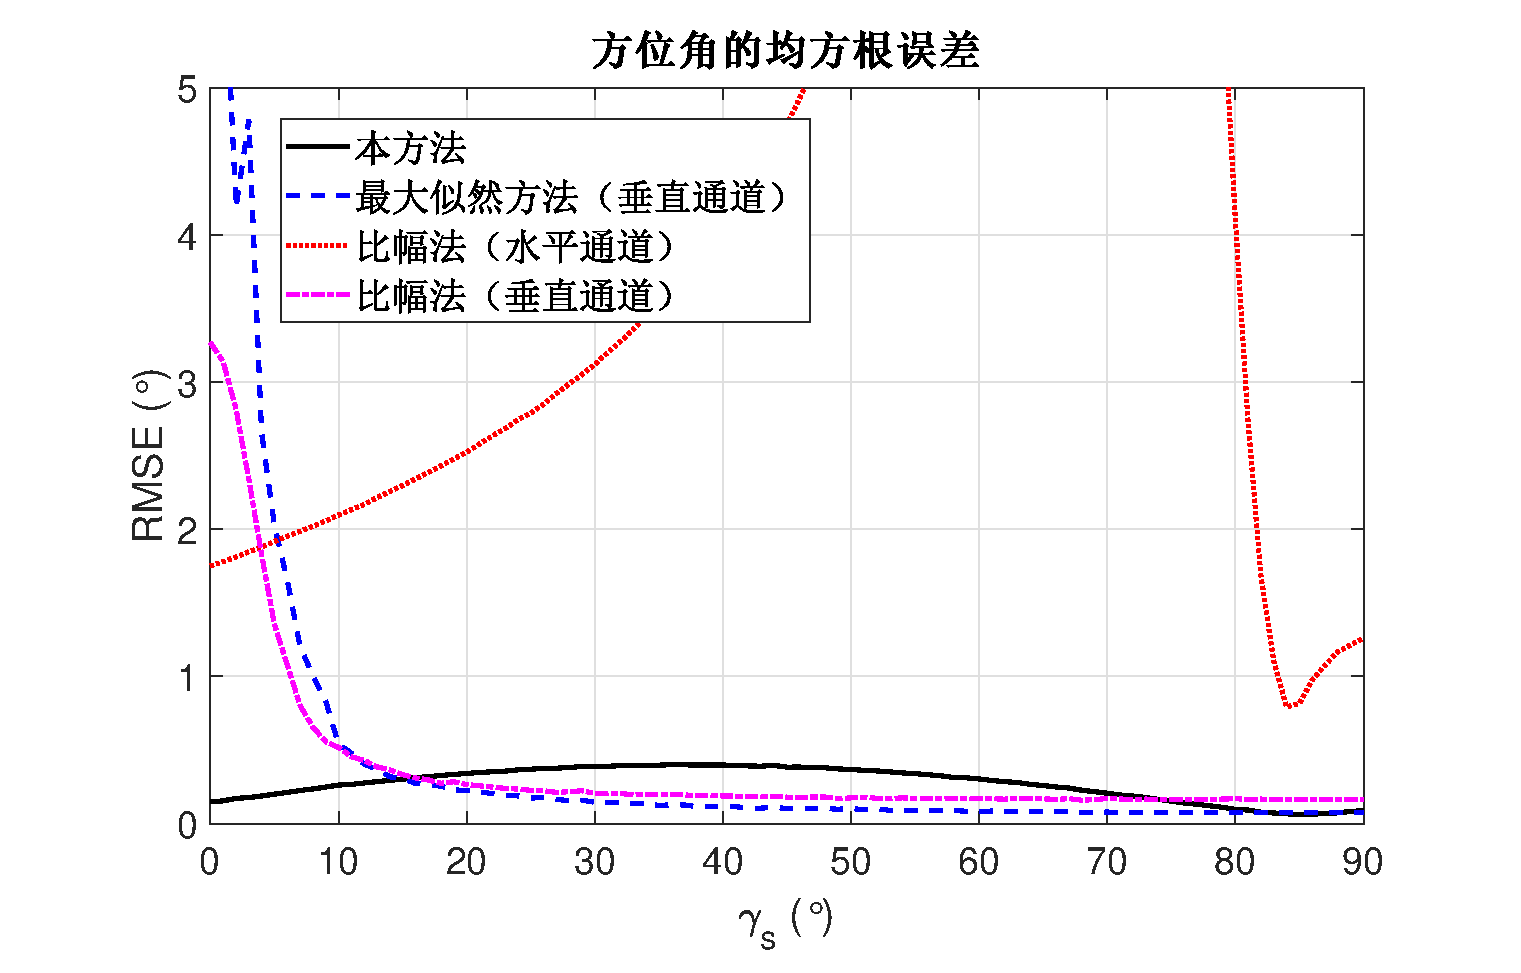
\includegraphics[scale=0.4]{pic/azimuth_RMSE_jammer_free.eps}
    }
    \floatcontinue
    \subfloat[]{
        \label{Polar_RMSE_jammer_free_b}
        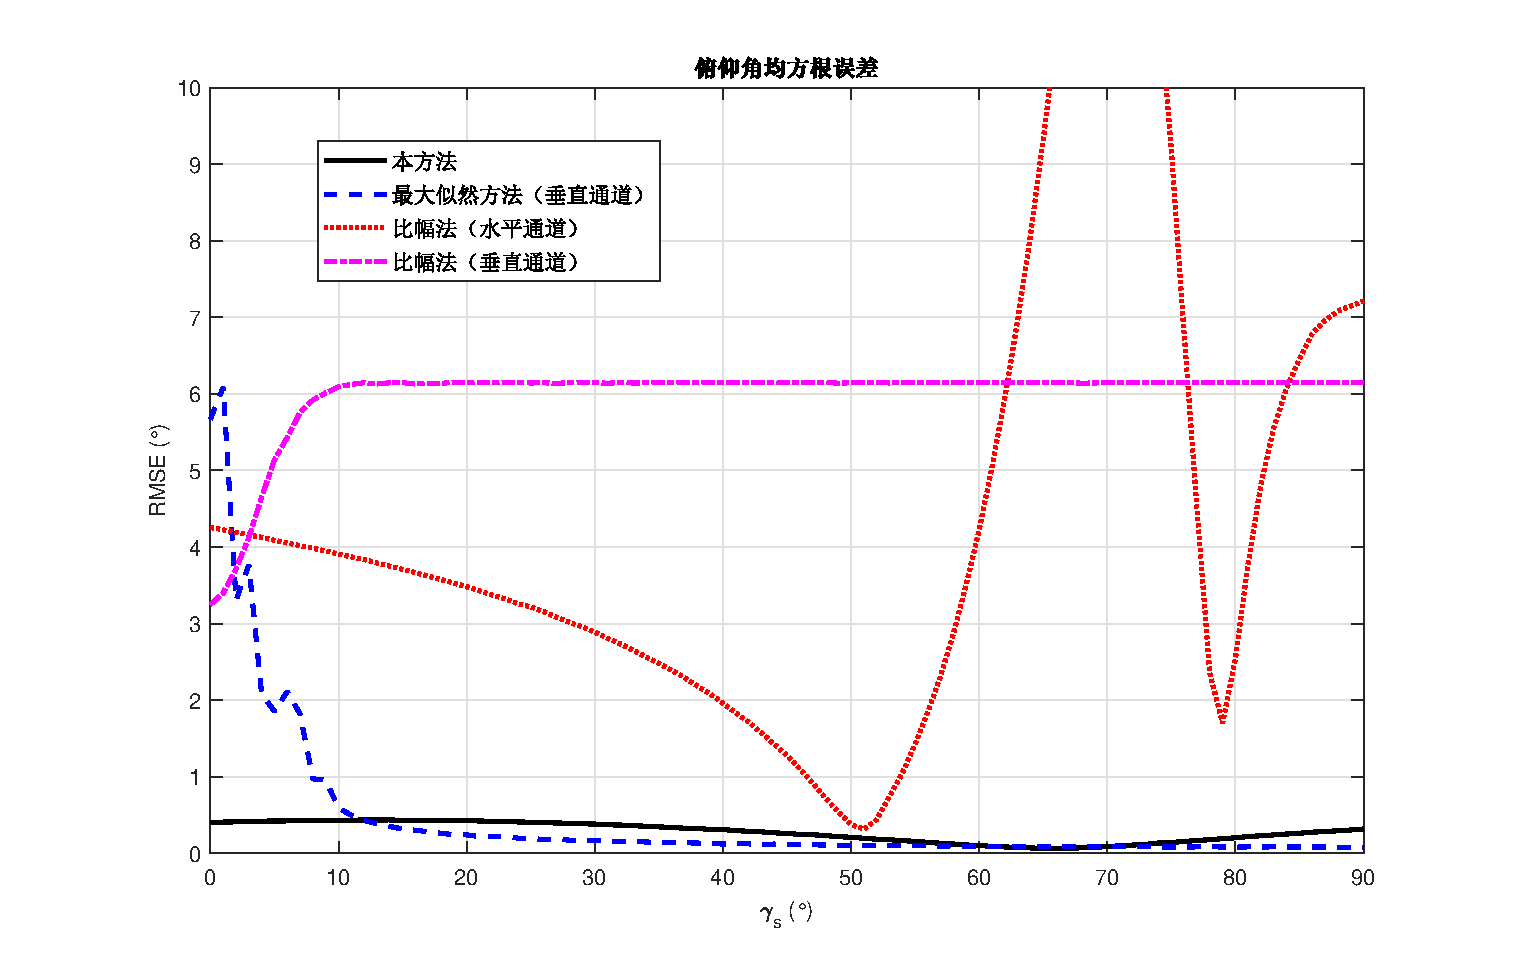
\includegraphics[scale=0.4]{pic/elevation_RMSE_jammer_free.eps}
    }
    \caption{无干扰条件下方向估计的RMSE。(a)方位角RMSE;(b)俯仰角RMSE}
    \label{Polar_RMSE_jammer_free}
\end{figure}

从图\ref{Polar_RMSE_jammer_free}中,我们可以注意到水平通道的比幅法几乎完全失效了。而垂直通道的最大似然方法和比幅法,
虽然在大部分区域的测向结果较为理想,但当期望信号的极化辅助角$\gamma_s$接近0时,垂直通道上的最大似然方法和比幅法都失效了,
这是因为当$\gamma_s$接近0时,期望信号的垂直极化分量$\exp(j\eta_s)\sin\gamma_s$也接近0,等效的使得垂直通道的极子
接收到的信号功率变得微弱,降低了信噪比。作为对照,我们提出的方法在极化辅助角$\gamma_s$
的整个定义域内都能得到较为理想的测向结果。

仿真B:存在一旁瓣干扰时的测向性能对比

在本次仿真中,我们探究存在旁瓣干扰时各算法的性能,考虑一个旁瓣干扰,以方位角$\theta_j=25^\circ$,
俯仰角$\phi_j=25^\circ$入射到该阵列上,它的极化辅助角$\gamma_j$为$40^\circ$,极化相位差$\eta_j$为$30^\circ$,
干噪比为55dB,期望信号与仿真A中相同。仿真结果对比如图\ref{Polar_RMSE_SLJ}所示。
\begin{figure}[h]
    \subfloat[]{
        \label{Polar_RMSE_SLJ_a}
        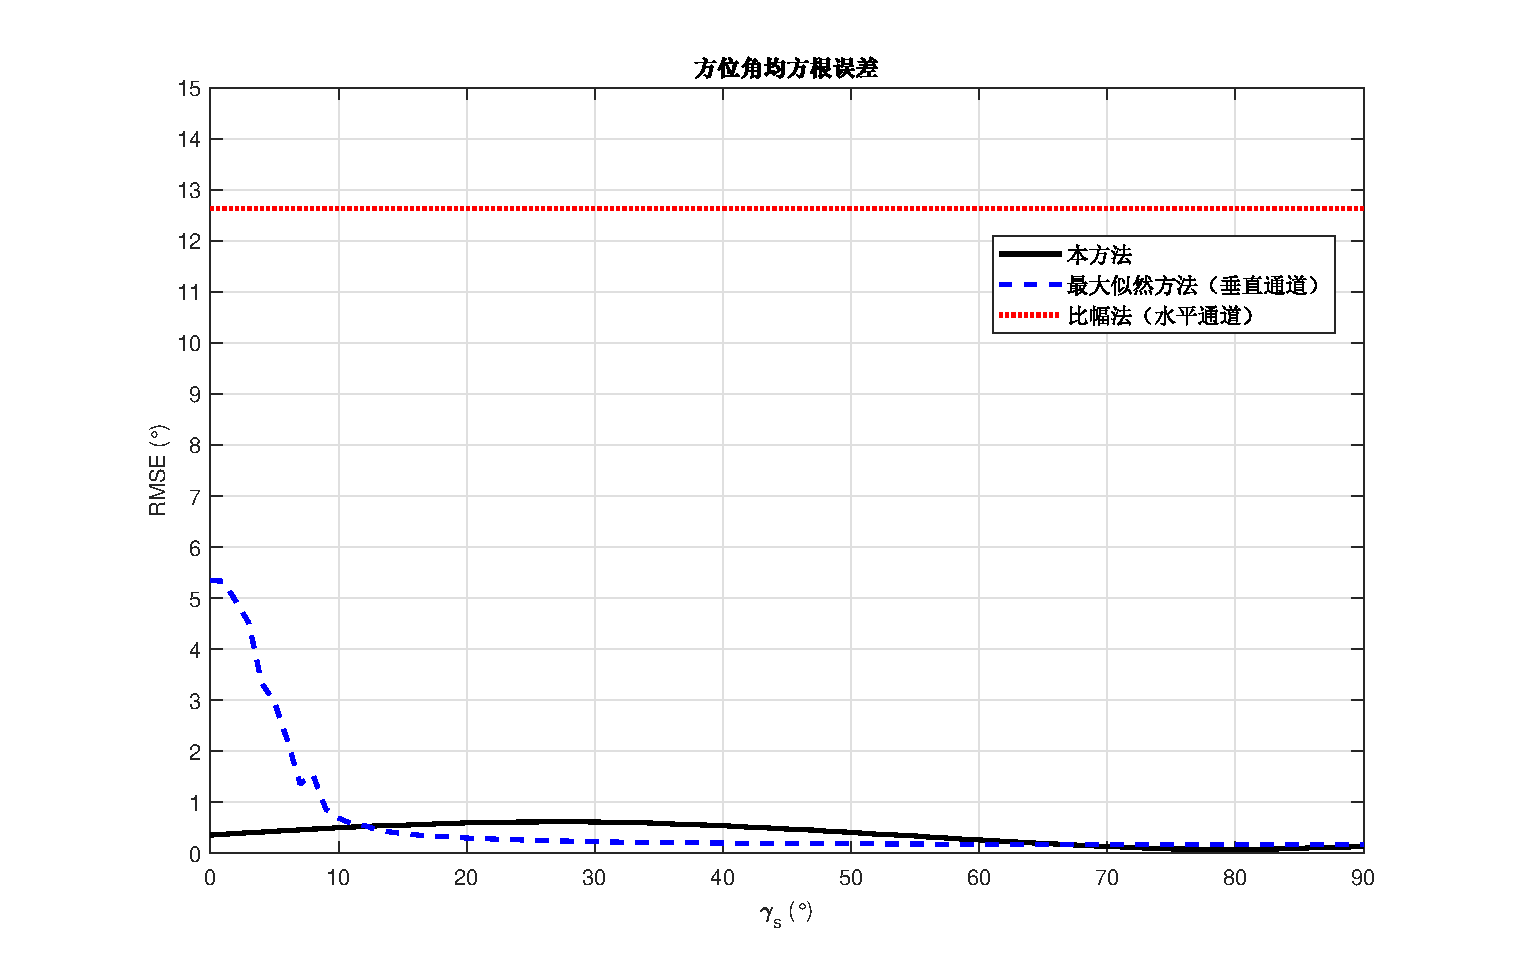
\includegraphics[scale=0.4]{pic/azimuth_RMSE_SLJ.eps}
    }
    \floatcontinue
    \subfloat[]{
        \label{Polar_RMSE_SLJ_b}
        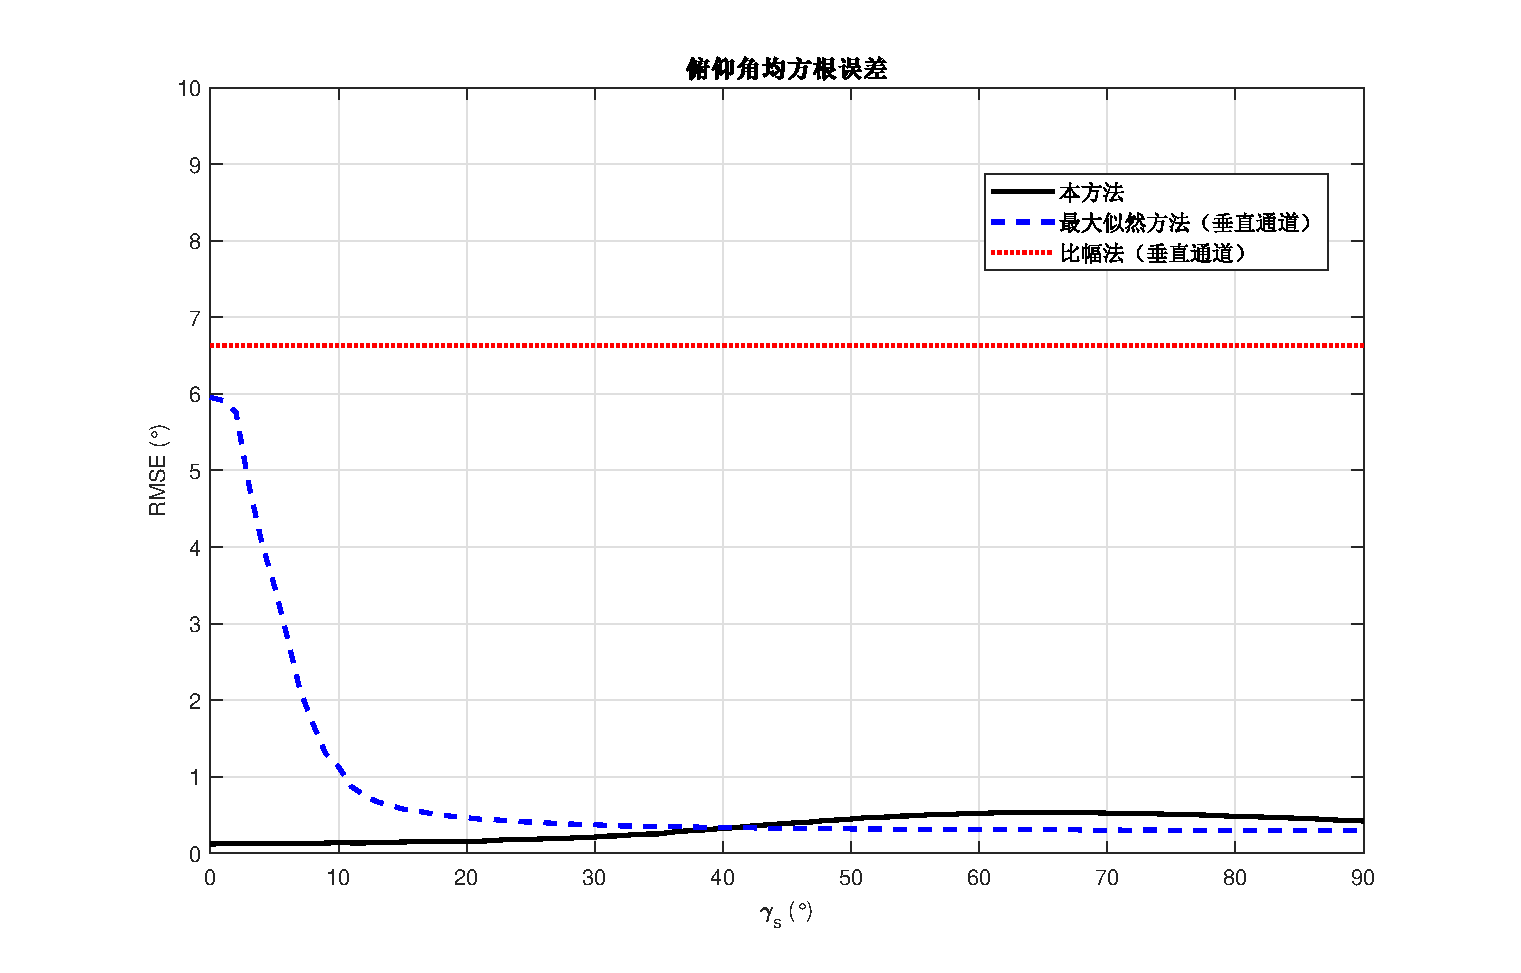
\includegraphics[scale=0.4]{pic/elevation_RMSE_SLJ.eps}
    }
    \caption{存在旁瓣干扰时的方向估计RMSE。(a)方位角RMSE;(b)俯仰角RMSE}
    \label{Polar_RMSE_SLJ}
\end{figure}

由于垂直通道上比幅法的RMSE远大于$10^\circ$,因此我们在对比图中不展示它。从图\ref{Polar_RMSE_SLJ}中我们可以看出,
旁瓣干扰的存在同样使得水平通道的比幅法失效了,这是因为比幅测向法是非自适应测向方法,无法应对旁瓣干扰。
而最大似然方法虽然能够有效的抑制旁瓣干扰,但当$\gamma_s$趋近于0时,它还是会失效。作为对比,我们的方法能够处理
旁瓣干扰,并且在$\gamma_s$的整个定义域上都有较为理想的结果。

仿真C:无干扰时的极化参数估计性能

在仿真C中,我们探究无干扰时本方法的极化参数估计性能。期望信号的极化相位差$\eta_s=0$,极化辅助角$\gamma_s$从
$0$变化到$\pi/2$,其余条件不变。极化参数的估计性能如图\ref{Polar_args_RMSE}所示。
\begin{figure}[h]
    \subfloat[]{
        \label{Polar_args_RMSE_a}
        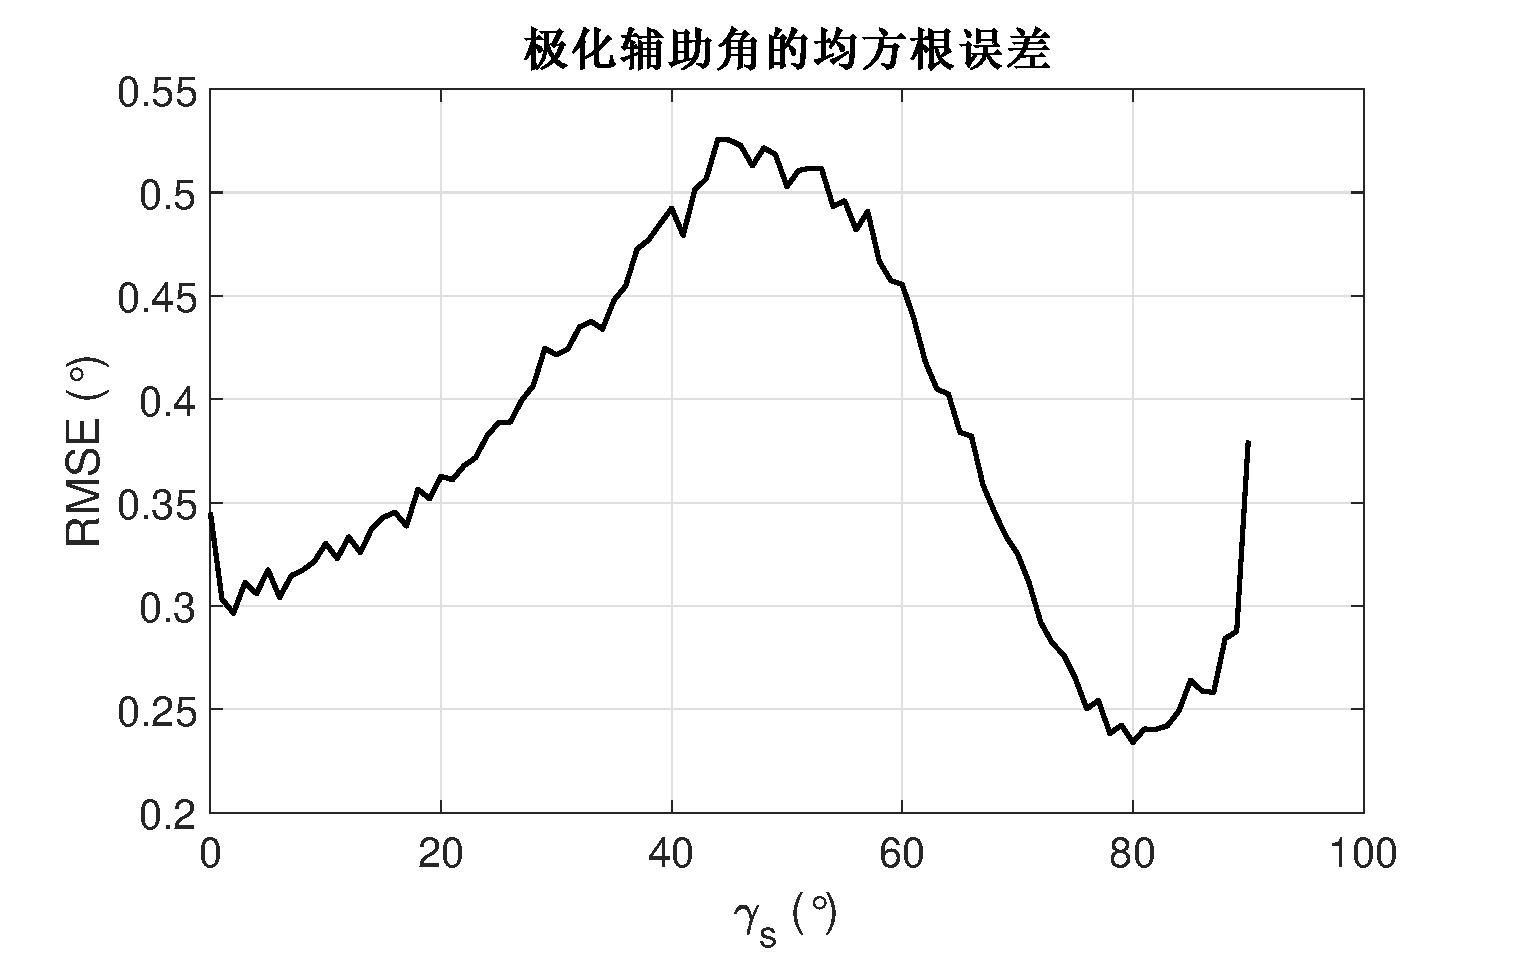
\includegraphics[scale=0.4]{pic/gamma_hat.eps}
    }
    \floatcontinue
    \subfloat[]{
        \label{Polar_args_RMSE_b}
        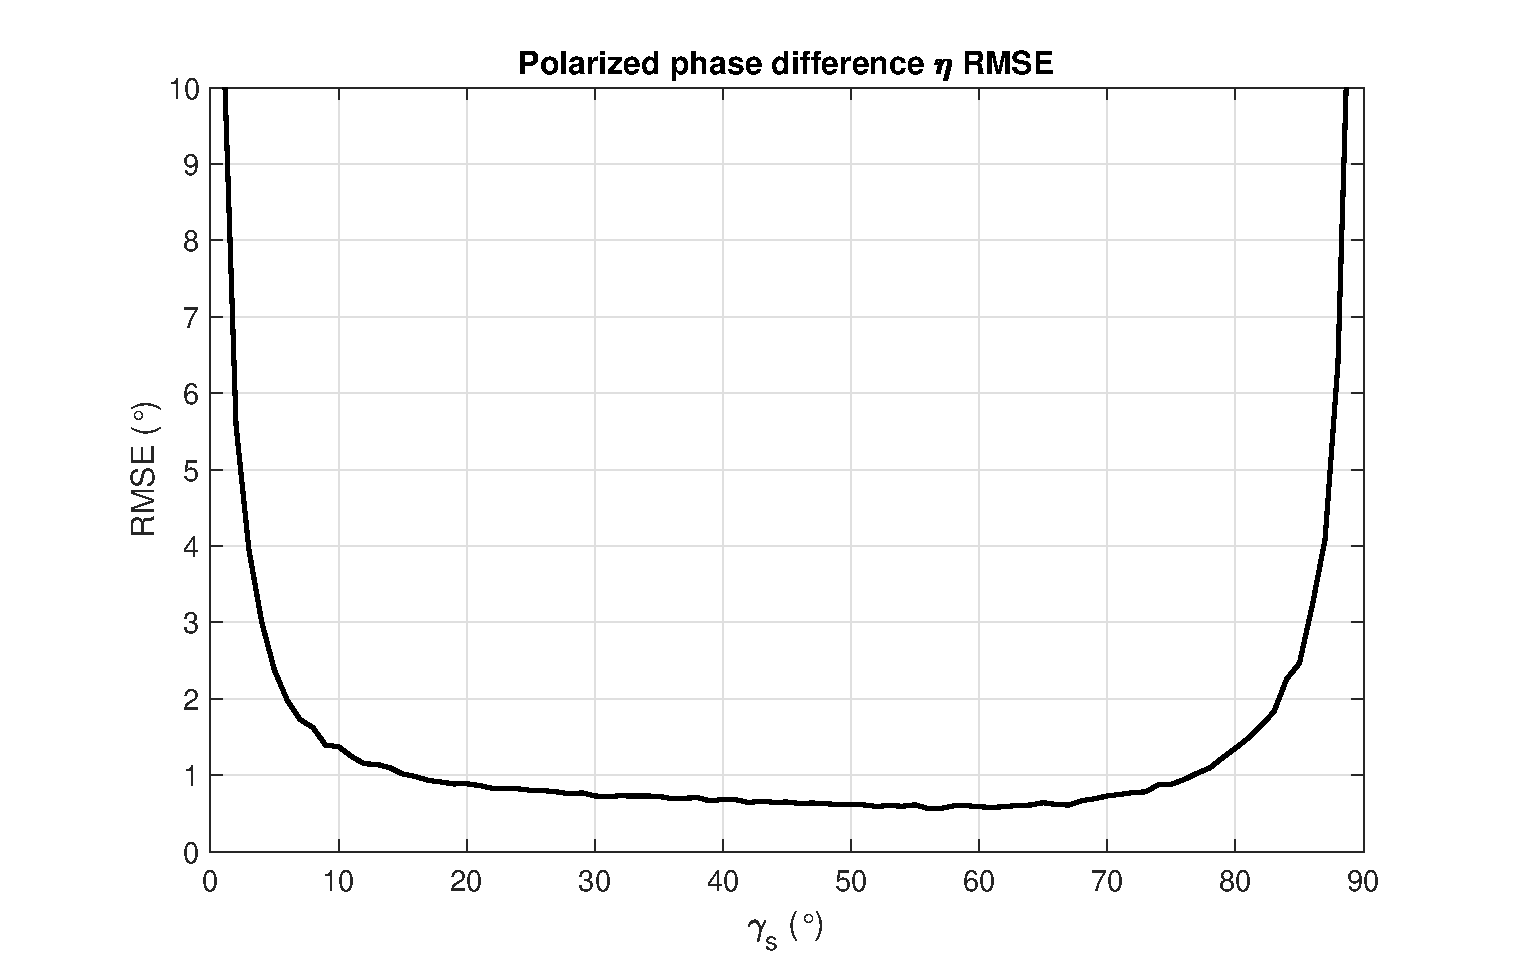
\includegraphics[scale=0.4]{pic/eta_hat.eps}
    }
    \caption{无干扰时的极化参数估计RMSE。(a)极化辅助角RMSE;(b)极化相位差RMSE}
    \label{Polar_args_RMSE}
\end{figure}

从图\ref{Polar_args_RMSE}中我们可以看出,在大部分情况下,最小二乘解都可以给出可接受的极化参数估计结果,
但是当极化辅助角$\gamma_s$接近0或者$\pi/2$时,期望信号的极化向量$\bm{h}$中有一个元素会趋近于0,
这使得式\eqref{polar_args_hat_arc}退化,无法估计出正确的极化相位差$\hat{\eta}_s$。
而其他传统单脉冲测向方法无法估计极化参数。

\section{本章小结}
本章中,我们介绍了极化相控阵模型,并给出了针对两种极化相控阵模型的单脉冲测向方法。
与传统的单脉冲阵列不同,极化相控阵将信号处理拓展到了极化域,把信号的极化信息也纳入了考虑。

我们给出了两种基本的极化相控阵信号模型,首先是任意极子朝向的信号模型,
其次是正交极子的信号模型。实际上正交机子的信号模式是第一种任意极子朝向信号模型的特殊情况,
即组成阵列的各个极子都沿着直角坐标系的轴线方向排列,在这种情况下,我们可以将多个极子的空域-极化域导向向量改写为
Kronecker积的形式,这样就可以将不同指向的几组极子分开,独立的看作几个通道。

因此,我们给出的第一种方法就是针对双正交极子极化阵列的信息融合方法,将双正交极子依照其极子朝向划分为水平极化通道和
垂直极化通道。由于上述Kronecker积的特性,分别对两个通道进行传统单脉冲测向(文中给出的是半阵法,亦可以使用别的传统单脉冲方法),
然后利用最大似然准则得到两个通道的信号功率估计值,并将其作为加权平均的权值,参与到最终估计量融合的过程中,得到最后的方向估计值。

第二中方法针对的是任意极子朝向的极化阵列。在这种模型下,由于阵元中的极子朝向不尽相同,因此无法像正交极子模型那样,
将它们划分为相对独立的几个通道。所有有必要采取一种联合估计方式来进行测向。因此我们从干扰叠加噪声的统计信息出发,
构造出关于极化参数和方向参数的似然函数,然后借助似然函数解出复振幅和极化分量的最小二乘解,并将其代入原似然函数中,
得到一个仅与方向参数有关的对数似然函数,最后借助牛顿公式,得到方向的估计量,并且可以估计值作为已知量,代入最小二乘解中,
得到极化参数的估计值。

\chapter{全文总结与展望}
\section{全文总结}
本文针对数字相控阵的单脉冲测向方法进行了深入的研究,研究内容包含以下几个部分。

1. 了解数字相控阵单脉冲测向的发展历史、国内外研究现状以及目前该领域的热点问题和面临的挑战,发掘深层次的研究意义。

2. 研究相控阵的基本信号模型,包括均匀线阵、均匀面阵、均匀面阵和共形阵,并研究了波束形成技术,以及三种传统单脉冲测向方法,
分别是半阵法、加权法和比幅测向法。其中半阵法只能用于均匀面阵和均匀线阵,加权法只能用于均匀线阵、均匀面阵和均匀圆阵,
而比幅测向法可以用于任意阵列。

3. 在传统单脉冲测向法中,除去加权法以外,都无法适用于强旁瓣干扰的场景。所以在这一部分中我们研究了三中抑制旁瓣干扰的方法,
它们分别是线性规划、差分进化和广义旁瓣对消方法。前两种方法都是静态波束权向量优化方法,与加权法类似,
设计一套满足技术指标的和差波束权向量,利用旁瓣抑制比抑制强旁瓣干扰,进而利用优化后和差波束的单脉冲比进行测向。
而广义旁瓣对消方法则是利用辅助阵列,使之阻塞期望信号但使强旁瓣干扰无失真的通过,进一步在输出端叠加主阵列输出与辅助阵列输出,
由于主阵列的波束与辅助阵列的波束中均含有旁瓣干扰,因此它们会叠加相消。而主阵列的波束中包含期望信号,
但期望信号在辅助阵列中被阻塞,因此叠加后的输出仍然保有期望信号。与传统方法类似,广义旁瓣对消仍然要结合静态和差波束权向量(如半阵法),
利用主阵列与辅助阵列叠加后的和差波束形成单脉冲比进行测向。

4. 研究自适应单脉冲测向方法,该方法与第三部分中的旁瓣抑制方法不同,是一种在线估计算法。它们充分利用了干扰叠加噪声的统计特性,
在线计算出实时的自适应和差波束权向量,或给出一种自适应单脉冲求解公式,在抑制主旁瓣干扰的同时测量期望信号的入射角度。
在这一部分中我们研究了四种自适应单脉冲测向方法,并对其中一种单脉冲测向方法进行了改进,极大的提高了它的测角精度。
第一种是最大似然方法,该方法借助似然函数和牛顿公式,估计出期望信号的入射角度。第二种是MVAM方法,该方法利用一阶泰勒展开公式,
重构出理想的单脉冲比,并给出了一种更为直接的估计公式。第三种是正交置零方法,该方法巧妙的利用了均匀面阵中方位角通道和俯仰角通道
的可分离性,对主瓣干扰进行抑制,再结合其他旁瓣干扰抑制方法,即可实现自适应单脉冲测向。
第四种是线性约束方法,该方法借助MVDR波束形成技术和LCMV结构,约束单脉冲比,求得自适应和差波束权向量,最后用于单脉冲测向。
最后,我们对线性约束方法进行了改进,利用SVD对约束矩阵进行近似处理,在提高测向精度的同时尽可能减少自由度的消耗。

5. 最后研究了极化相控阵模型下的单脉冲测向问题。在这一部分中,我们将阵列信号处理扩展到了信号的极化域。
与传统的相控阵不同,在该模型下,期望信号的电磁波极化模式也被纳入考虑。我们首先研究了极化相控阵的信号模型,
依据极子摆放的方式,我们可以将其归为两类,第一类是组成阵列的极子摆放方式不尽相同,即任意极子的极化相控阵。
第二类是组成阵列的极子摆放方式都相同,一般情况下,我们考虑正交极子模型,即阵列中的所有极子都沿着直角坐标系的轴线方向分布,
在这种情况下,摆放方式相同的极子可以被划分为同一个通道,各个通道的处理过程相对独立。我们首先针对正交极子极化阵列的测向展开研究,
由于其通道的独立性,我们介绍了一种多通道信息融合的测向方法,该方法首先在各个同上上做传统单脉冲测向,然后依据最大似然准则,
估计出各个通道的信号功率,最后以信号功率作为权值,对估计值做加权平均,得到最终估计量。然后我们针对任意极子的极化相控阵模型,
提出了一种联合估计方法,由于该模型下各个通道的耦合性,我们从干扰叠加噪声的统计特性出发,构造似然函数,首先利用最小二乘法
消去关于信号复振幅及其极化参数,将对数似然函数转变为一个只与入射角度有关的函数,然后借助牛顿公式,求得方位角和俯仰角,
最后将方位角和俯仰角作为已知量,重新代入信号向量得最小二乘解,求得其极化参数。

综上所述,本文完成了预定研究计划。改进了一种自适应单脉冲测向方法,提升了精度,该方法不受限于阵列结构,可用于共形阵。
针对任意极子的极化阵列给出了一种联合估计方法,得到该模型下入射角度和极化参数的估计值,
并且该算法不需要已知信号的极化信息,不受限于具体的阵列形式。

\section{后续工作展望}
本文中,针对任意极子极化相控阵提出的联合估计方法,虽然能够在未知极化参数的条件下得到较好的估计结果,
但在低信噪比时的测角性能还有待提高。其次,该算法在求解牛顿法所必要的海森矩阵时,没有对对数似然函数的二阶导数进行恰当的近似,
而是直接采用真实值参与估计,因此总体计算量较大。另外,由于时间有限,暂且没有对该算法的性能做理论分析,也没有考虑不同
信源模型下的CRLB。最后,可以考虑用交替方向乘子法(ADMM)求解该似然函数,用多步迭代方法,交替迭代方向参数和极化参数,
可能会得到性能更优的结果。

\thesisacknowledgement
在攻读硕士学位期间,首先衷心感谢我的导师XXX教授

\thesisappendix

\chapter{中心极限定理的证明}

\section{高斯分布和伯努利实验}


% Uncomment to list all the entries of the database.
% \nocite{*}

\thesisbibliography{reference}


% Uncomment following codes to load bibliography database with native
% \bibliography command.

% \nocite{*}
% \bibliographystyle{thesis-uestc}
% \bibliography{reference}

% \thesisaccomplish{publications}

% \thesistranslationoriginal
% \section{The OFDM Model of Multiple Carrier Waves}

% \thesistranslationchinese
% \section{基于多载波索引键控的正交频分多路复用系统模型}

\end{document}
